%\documentclass[conf]{new-aiaa}
\documentclass[journal]{new-aiaa}
\usepackage[utf8]{inputenc}

\usepackage{graphicx}
\usepackage{amsmath}
\usepackage[version=4]{mhchem}
\usepackage{siunitx}
\usepackage{longtable,tabularx}
\usepackage{fixfoot}

\usepackage{caption}
\usepackage{subcaption}
\usepackage{upgreek}
\usepackage{overpic}
\usepackage{xcolor}

\setlength\LTleft{0pt} 

\makeatletter
\patchcmd\@fixed@footnote
  {\protected@xdef\@thefnmark{\csname @#1@fftn@footnote\endcsname}}% search
  {\protected@xdef\@thefnmark{%
     \expandafter\@fnsymbol\csname @#1@fftn@footnote\endcsname}}% replace
  {}{}% success/failure
\makeatother

\DeclareFixedFootnote{\noteA}{Graduate Research Assistant, Member AIAA}
\DeclareFixedFootnote{\noteB}{Associate Professor, Associate Fellow AIAA}
\DeclareFixedFootnote{\noteC}{Professor, Associate Fellow AIAA}


\title{Combined PIV-PLIF of High-Speed Cavity-Stabilized Combustion}

\author{Clayton M. Geipel\noteA, Damien A. Lieber\noteA, and Christopher P. Goyne\noteB}
\affil{University of Virginia, Department of Mechanical and Aerospace Engineering\\Charlottesville, Virginia 22904}
\author{Andrew D. Cutler\noteC}
\affil{The George Washington University, Department of Mechanical and Aerospace Engineering\\
Washington, District of Columbia 20052}

\begin{document}

\maketitle

\begin{abstract}
Combined particle image velocimetry and hydroxyl planar laser induced fluorescence measurements are conducted in a dual-mode combustor operated in ramjet mode, with premixed ethylene-air combustion stabilized by a cavity. The cavity is scaled to be suitable for direct numerical simulations. Simultaneous measurements of instantaneous flow velocities and locations of flame products enable deeper insights into turbulence-flame interactions. The shear layer originating at the cavity leading edge generates periodic vortical structures and a wrinkled flame. Under the shear layer, an unsteady recirculation zone promotes mixing of cavity-generated combustion products with the free stream. A description of periodic, unsteady combustion in the cavity is proposed. The cycle starts with a trapped recirculation vortex in the cavity near the leading edge which grows as it accumulates mass and heat. This unsustainable state triggers splitting of the vortex and detachment of the shear layer from the cavity ramp. Combustion products and the downstream vortex are ejected downstream from the cavity and the flame is broken. The cycle is completed when the shear layer reattaches and again forms a trapped recirculation vortex. This unsteady combustion cycle may be phase-coupled with a global flame instability such as thermoacoustic oscillations.
\end{abstract}

% \section*{Nomenclature}

% {\renewcommand\arraystretch{1.0}
% \noindent\begin{longtable*}{@{}l @{\quad=\quad} l@{}}

% $\Phi_g$ & global fuel-air equivalence ratio \\
% $H$ & cavity height \\
% $L$ & cavity length \\
% $M$ & Mach number \\ 
% $m$ & image magnification \\
% $Re$ & Reynolds number \\
% $\Delta t$ & time between PIV acquisitions \\
% $U_x,\ U_y$ & velocity components \\
% $U_P,\ U_R$ & velocities conditioned on products and reactants \\
% $x,\ y$ & coordinates with origin at cavity leading edge \\

%\end{longtable*}}

\section*{Introduction}
\lettrine{U}{nderstanding} the fundamental physics governing cavity flameholders is critical to the development of high-speed air-breathing propulsion systems such as hydrocarbon-fueled dual-mode scramjets. Hydrocarbon fuels are easier to store and handle than hydrogen and therefore considered more practical. In the absence of a flameholder in the engine, the longer reaction times of these fuels inhibit the complete release of their chemical energy before exiting the scramjet. Cavities solve this problem by locally increasing the residence time, creating a shear layer and flow recirculation \citep{Ben-YakarHanson2001}. Combustion radicals are produced in the cavity before being diffused through turbulent fluctuations across the shear layer and intermittently ejected into the main flow \citep{Kirik2017}. In addition to applications in scramjet combustors, cavity flameholders enable fundamental research on high-speed combustion by establishing in a premixed free stream a flame with a relatively large normal velocity. The intricate interactions between the flow unsteadiness and chemical reactions are however not fully understood and warrant further investigation. In particular, combustion instabilities in premixed dual-mode scramjet flowpaths with a cavity flameholder are an area of continuing research \citep{WangWangSun2014}. The problem is critical to enabling operational engines and reliable computational fluid dynamics (CFD) simulations.
 
Scramjet combustors with flush or ramp injectors have been extensively studied \citep{RockwellGoyneRiceEtAl2014, LaurenceLieberSchrammEtAl2015, LePichonLaverdant2016, FangHong2018}. High-speed cavity flameholders became a topic of interest more recently. Tuttle et al.
\cite{TuttleCarterHsu2014} published the first study of these flameholders operating in scram-mode by implementing particle imaging velocimetry (PIV) and comparing results to a separate planar laser-induced fluorescence (PLIF) study in order to investigate the dependence of velocity behavior on the heat release in the cavity and shear layer. These authors found a strong coupling between various velocimetry statistics and heat release rates, noting the value simultaneous PIV and PLIF would hold in order to clarify coupling between heat release and velocity.
Research on premixed and dual-mode scramjet combustors with a cavity flameholder is particularly recent; the only study known to the authors \cite{KirikGoyneMcDanielEtAl2017} was conducted on the same facility as the present work but with a larger cavity and flowpath. The investigators characterized premixed cavity aerodynamics and its relation to both the shock train upstream location and the fuel equivalence ratio by conducting PIV and PLIF of the hydroxyl (OH) radical as separate experiments. In particular, their comparison of the peak fluctuations in velocities and relative OH levels suggest an unsteady combustion process whereby pockets of combustion products produced near the ramp are intermittently ejected into the main duct flow.


Chemiluminescence imaging of the CH* radical has been performed \cite{AllisonFredericksonKirikEtAl2017}  on a similar cavity flameholder flowpath in the University of Virginia Supersonic Combustion Facility (UVaSCF). That study suggested a characteristic frequency of 340 Hz in the CH* signal and flame brush, which is likely due to acoustic waves between the shock train and the thermal throat. Phase-coupled addition of energy to these waves occurs due to heat addition by combustion in the flow between the cavity and the thermal throat. 
Stable combustion is desired for operational application on aircraft, hence the mechanisms driving combustion oscillations warrant further investigation.
\citet{WangWangSun2014} reviews recent progress on combustion oscillations in dual-mode scramjets and highlights their variety and complexity. Thermoacoustic oscillations are on the order of hundreds of Hz while the cavity shear layer oscillates at higher frequencies, particularly for low heat release rates.  
\citet{LinJacksonBehdadniaEtAl2010} used a high-frequency pressure sensor and theoretical/numerical analysis to study oscillations in a dual-mode, non-premixed scramjet flowpath. For the conditions closest to the present work with a single-sided injection from the cavity wall, a dominant frequency of 368 Hz is measured. The oscillation is attributed to acoustic-convective wave interactions between the terminal shock and the thermal throat and between the fuel injectors and the thermal throat. In this case, the oscillation in local heat release rate sends an acoustic wave upstream, which modifies fuel penetration and mixing. 
Hybrid large eddy simulation (LES)/Reynolds-averaged Navier-Stokes simulations by \citet{ramesh2015large} of a dual-mode premixed flowpath with a cavity flameholder observed a 357 Hz cyclic combustion pattern. While the non-satisfaction of the Rayleigh criterion and the large amplitude of the oscillations hint at a computational aberration, their work nonetheless gives valuable insights into interactions between the shock train and the cavity-stabilized flame. These authors report an oscillation in heat release. Mass accumulates periodically in the cavity, reducing heat release, increasing cavity pressure, and causing a normal shock wave to propagate upstream. Increasing heat release is associated with a positive mass flow rate due to ejection events and higher duct flow velocities due to thermoacoustic fluctuations.
Non-simultaneous PIV and PLIF measurements on scramjet combustors also observed hints at an oscillatory combustion pattern. 
Tuttle et al. \cite{TuttleCarterHsu2014} suggest an intermittently-stable shear layer flame driving cavity combustion dynamics in a supersonic flow, whereby heat release influences the shear layer impingement location and the formation of the recirculation-zone eddy structures.
Kirik \cite{Kirik2017} observed that locations with the strongest turbulent fluctuations are adjacent to locations with high OH concentration fluctuations, hinting at the intermittent release of high-temperature products and radical species from the cavity.  
Tuttle et al. \cite{TuttleCarterHsu2014} and Kirik \cite{Kirik2017} noted that simultaneous PIV and PLIF would help understanding of the instantaneous mechanism behind the unsteady combustion process. 


%Cavities without combustion have been extensively studied and provide additional material to interpret the mechanisms behind reacting cavity instabilities. Gharib and Roshko \cite{GharibRoshko1987} report on a locked vortex configuration within the cavity corresponding to stable flow. This configuration is however established at the cost of low mass exchange between the cavity and the duct flow. 
%Ben-Yakar and Hanson \citep{Ben-YakarHanson2001}, in a comprehensive review about cavity flows, described the phenomenon of longitudinal oscillations in non-combusting rectangular cavity flow. These oscillations are driven by shear layer unsteadiness adding and removing mass at the cavity closeout. When the freestream flow enters the cavity at the impingement point, a compression wave propagates upstream, impacts the front wall, and generates small vortices at the leading edge. These eddies are in turn convected downstream, being amplified along the way. The cycle ends with vortex shedding, ejecting the mass initially added. Suppression of these cavity oscillations may be achieved with an oblique closeout wall to prevent the reflection of acoustic waves, as implemented in the present flowpath geometry.
%Low speed reacting flows in closed cavities were studied by \cite{XavierVandelGodardEtAl2016}, who resolved a full instability cycle with combined kHz PIV-PLIF. These authors highlighted the complex coupling between shear layer instabilities and the observed pulsed combustion regime. A stable combustion mode was reached at an increased free stream momentum relative to cavity injection momentum, which contains the cavity flow and constrains combustion within the shear layer. They suggested that large velocity fluctuations between the cavity and the main flow cause full shear layer modifications.

While separate PIV and PLIF measurements can give important insights by relating key turbulence characteristics with combustion-related statistics, they are limited by their temporally-uncorrelated nature. As a result, the analysis is constrained to relating independent statistical quantities. In addition, small variations within or between runs in total pressure, total temperature, or equivalence ratio further add to the limitations of this approach. In contrast, PIV-PLIF enables measurements that are correlated in time and space, providing deeper insight into the coupling between combustion physics and fluid mechanics \citep{TanahashiMurakamiChoiEtAl2005, GambaClemensEzekoye2013, XavierVandelGodardEtAl2016, FangHong2018}. 
The fundamental added value of PIV-PLIF is the knowledge of the distribution of products and reactants relative to the velocity fields for each instantaneous measurement, which is exploited in several ways. First, the velocity field can be divided into products and reactants domains --- i.e. conditional velocities --- from which stem conditional statistics, e.g. conditional means. 
Second, the instantaneous OH region boundaries from the PLIF signal approximate the local flame curvature and angle, which can then be related to the flow swirl, turbulence intensity, and direction. 
Third, knowledge of both the instantaneous flow dynamics and flame location provides complementary knowledge to characterize the flame anchoring process in terms of temporal dynamics. 
By leveraging the unique capabilities of simultaneous PIV-PLIF listed above, the present work aims to quantify the key characteristics of the chemically-reacting flow field of dual-mode cavity flameholders.

This work provides the first dataset of correlated velocimetry and OH distributions including conditional velocimetry statistics for numerical studies, to better understand flameholding mechanisms at play in a cavity-stabilized flame in a dual-mode scramjet operating in ramjet mode. In this mode, a shock train upstream of the combustor terminates in a normal shock, resulting in subsonic flow in the combustor. In particular, the mass transfer across the cavity boundary, the conditional velocimetry are investigated through mean and RMS velocity fields, the turbulent kinetic energy, and the turbulence intensity for both the full velocity field and conditional velocities; as well as the characterization of the cavity in terms of the recirculation regions,
shear layer impingement location, flame anchoring location, and temporal dynamics. In addition, the mass transfer of products and reactants at the cavity interface will be estimated based on the average transverse conditional velocities. 

The present work is part of a larger collaborative effort to deepen the fundamental understanding of cavity-stabilized combustion including its relation with flow compressibility and heat release rates. To that end, simultaneous PIV and OH PLIF, hereafter PIV-PLIF, are conducted on a high-speed reacting cavity flow. PIV-PLIF measurement has the advantages over separate measurement that flow-chemistry coupling is investigated with instantaneous measurements and complementary validation metrics are provided to companion CFD work. In particular, direct numerical simulations (DNS, discussed in \cite{rauch2018dns}) are being conducted parallel to the present experimental work to gain insights at the finest spatio-temporal scales. 

Because the cavities and flowpaths investigated previously were too large for feasible DNS computational times, the UVaSCF \cite{KraussJ.McDaniel1992, McDanielGoyneBrynerEtAl2005} has been modified to host a small-scale cavity flameholder as detailed in \cite{LieberGoyneRockwellEtAl2018a}. This cavity provides a smaller computational domain for CFD work, such that DNS is feasible with currently-available computing resources \cite{rauch2018dns}. The results presented below therefore constitute the first published reference dataset on a high-speed reacting cavity flow that may be computed using DNS. The inflow to the cavity has been characterized with high-resolution PIV in a separate study \cite{LieberThesis}.

The paper is structured as follows. First, the combined setup and post-processing are summarized. Second, the DNS-friendly, scaled-down, and immersed cavity flow is characterized with statistics and key values provided as references for CFD work. Finally, combustion dynamics are investigated with instantaneous measurements and a hypothetical combustion cycle is suggested for dual-mode scramjet cavity flameholder instability.

\section*{Method and Setup}\label{sec:ch3_method_setup}

\subsection*{Flow configuration and experimental setup}
Measurements are conducted on the flowpath detailed in \cite{LieberGoyneRockwellEtAl2018a} and depicted in Fig. \ref{fig:ch3_flowpath}. The flow into the scramjet had total temperature 1200 K and total pressure 300 kPa. An immersed insert with in the combustor section hosted a small open cavity flameholder. The cavity had a height $H$ of 3 mm and a closeout ramp angled at 22$^\circ$. The total length $L$ of the cavity from the step to the downstream end of the ramp was 18 mm. This cavity presents a smaller volume of interest for high-fidelity simulations; it was designed so that DNS investigations of the immediate vicinity of the cavity are feasible.  Upstream of the cavity is a short length of constant area duct of height 15 mm, width 38 mm, and length 30 mm with a thin boundary-layer on the cavity side \citep{LieberThesis}. Downstream of the cavity, a 2.9$^\circ$ divergence delays thermal choking. The streamtube captured between the cavity wall of the insert and the opposing wall of the duct merges with the main flow in the main flowpath extender. 

Measurements are acquired in a field of view (FOV) spanning the cavity as shown in Fig. \ref{fig:ch3_FOVs}. The cartesian coordinate system used in the following originates at the center of the cavity leading edge, with $\vec{x}$ along the streamwise axis and $\vec{y}$ along the transverse axis as illustrated in Fig. \ref{fig:ch3_FOVs}.

\begin{figure}[!hbt]
\centering
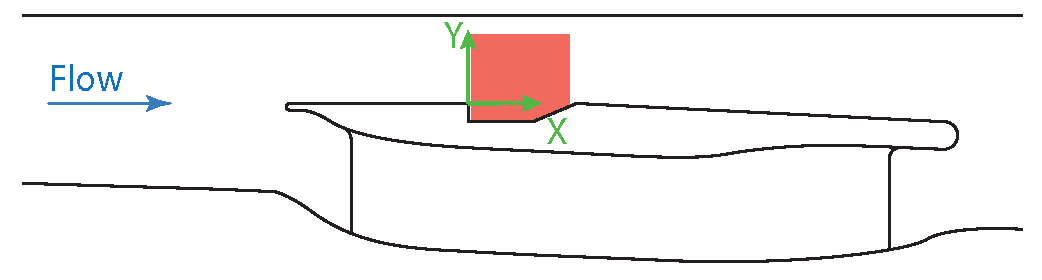
\includegraphics[width=3.25in, trim=0.3in 0in 0.57in 0in, clip]{figures/FOVs/aaArtboard2.png} %pdfcrop
\caption{Field of view of the present work relative to the flameholder.}\label{fig:ch3_FOVs}
\end{figure}

Ethylene fuel is injected from a row of three sonic injectors at 90$^\circ$ to the freestream into the main flowpath isolator to provide a global equivalence ratio of $\Phi_g=0.47$  \cite{RockwellGoyneChelliahEtAl2017}, which corresponds to the highest heat release rate attainable in the facility. The fuel is premixed by the turbulence generated by the isolator shock train. An air throttle at $x/H=57$ provides back pressure; it is set to the minimum flow rate at which combustion stability is maintained. In this configuration, the shock train leading edge is located near near $x/H=-140$. The local Mach number in the combustor was 0.66 (as calculated by a one-dimensional model of the facility isolator \cite{HeiserPrattDaleyEtAl1994}).

\begin{figure*}[!hbt]
\centering
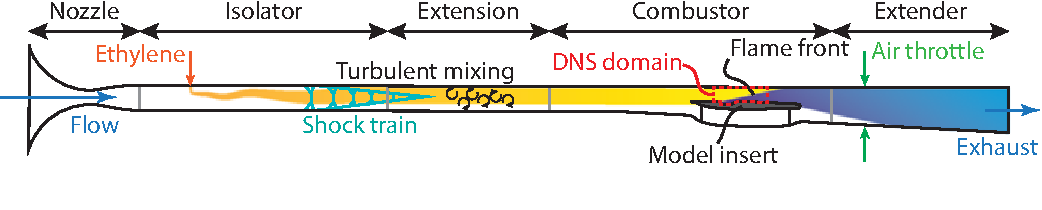
\includegraphics[width=6.5in]{figures/PIV-PLIFsetup/pivplifSmallcavity-crop.pdf} %pdfcrop
\caption{Schematic of the flow path.}\label{fig:ch3_flowpath}
\end{figure*}

The hardware and software system for the PIV-PLIF measurements is illustrated in Fig. \ref{fig:ch3_method_setup}. 
Both the PIV and OH-PLIF measurements are made on the duct spanwise center-plane, relying on the assumption of nominally two-dimensional flow in the cavity, which is consistent with a previous CFD study \cite{ramesh2015large}. The PIV and PLIF systems are run from a common external signal generator. The signal generator is set for the PLIF laser pulse to occur half-way between the two PIV laser pulses as measured by a photodiode. 
The PIV laser is a double-cavity, 10 Hz Spectra Physics PIV-400 Nd:YAG laser delivering two 532 nm-pulses of 500 mJ each, with inter-pulse delays of $\Delta t = 300$ ns. In order to maintain the fluence at the mirrors and model below damage thresholds, 95\% of the energy is dumped using beam splitters. To generate the PLIF laser beam, a Sirah Cobra Stretch dye laser with a mixture of Rhodamine 590 and Rhodamine 610 dyes output a 283.55 nm, 15 mJ/pulse beam to excite the Q$_1$(8) transition of OH \citep{GeipelRockwellChelliahEtAl2017}. The OH-PLIF signal is used as an indicator for the presence of combustion products. The PIV and PLIF laser beams are overlapped using a dichroic filter before the sheet-forming optics. The laser sheet is formed with telescoping optics to a constant height $\sim 25$ mm. To measure the thicknesses of the laser sheets, a portion of each beam was split off after the final focusing lens and was directed through neutral density filters and onto a Point Grey Blackfly CCD camera sensor. The PIV laser sheets are $\sim 140~ \mathrm{\upmu m}$ thick, while the PLIF laser sheet is $75~ \mathrm{\upmu m}$ thick, as measured by full-width at half-maximum at the sheet waist (see Fig. \ref{fig:ch3_meas_LS_thick}). The laser sheets are verified to be coplanar with negligible change in thickness across the FOV.
\begin{figure*}
\centering
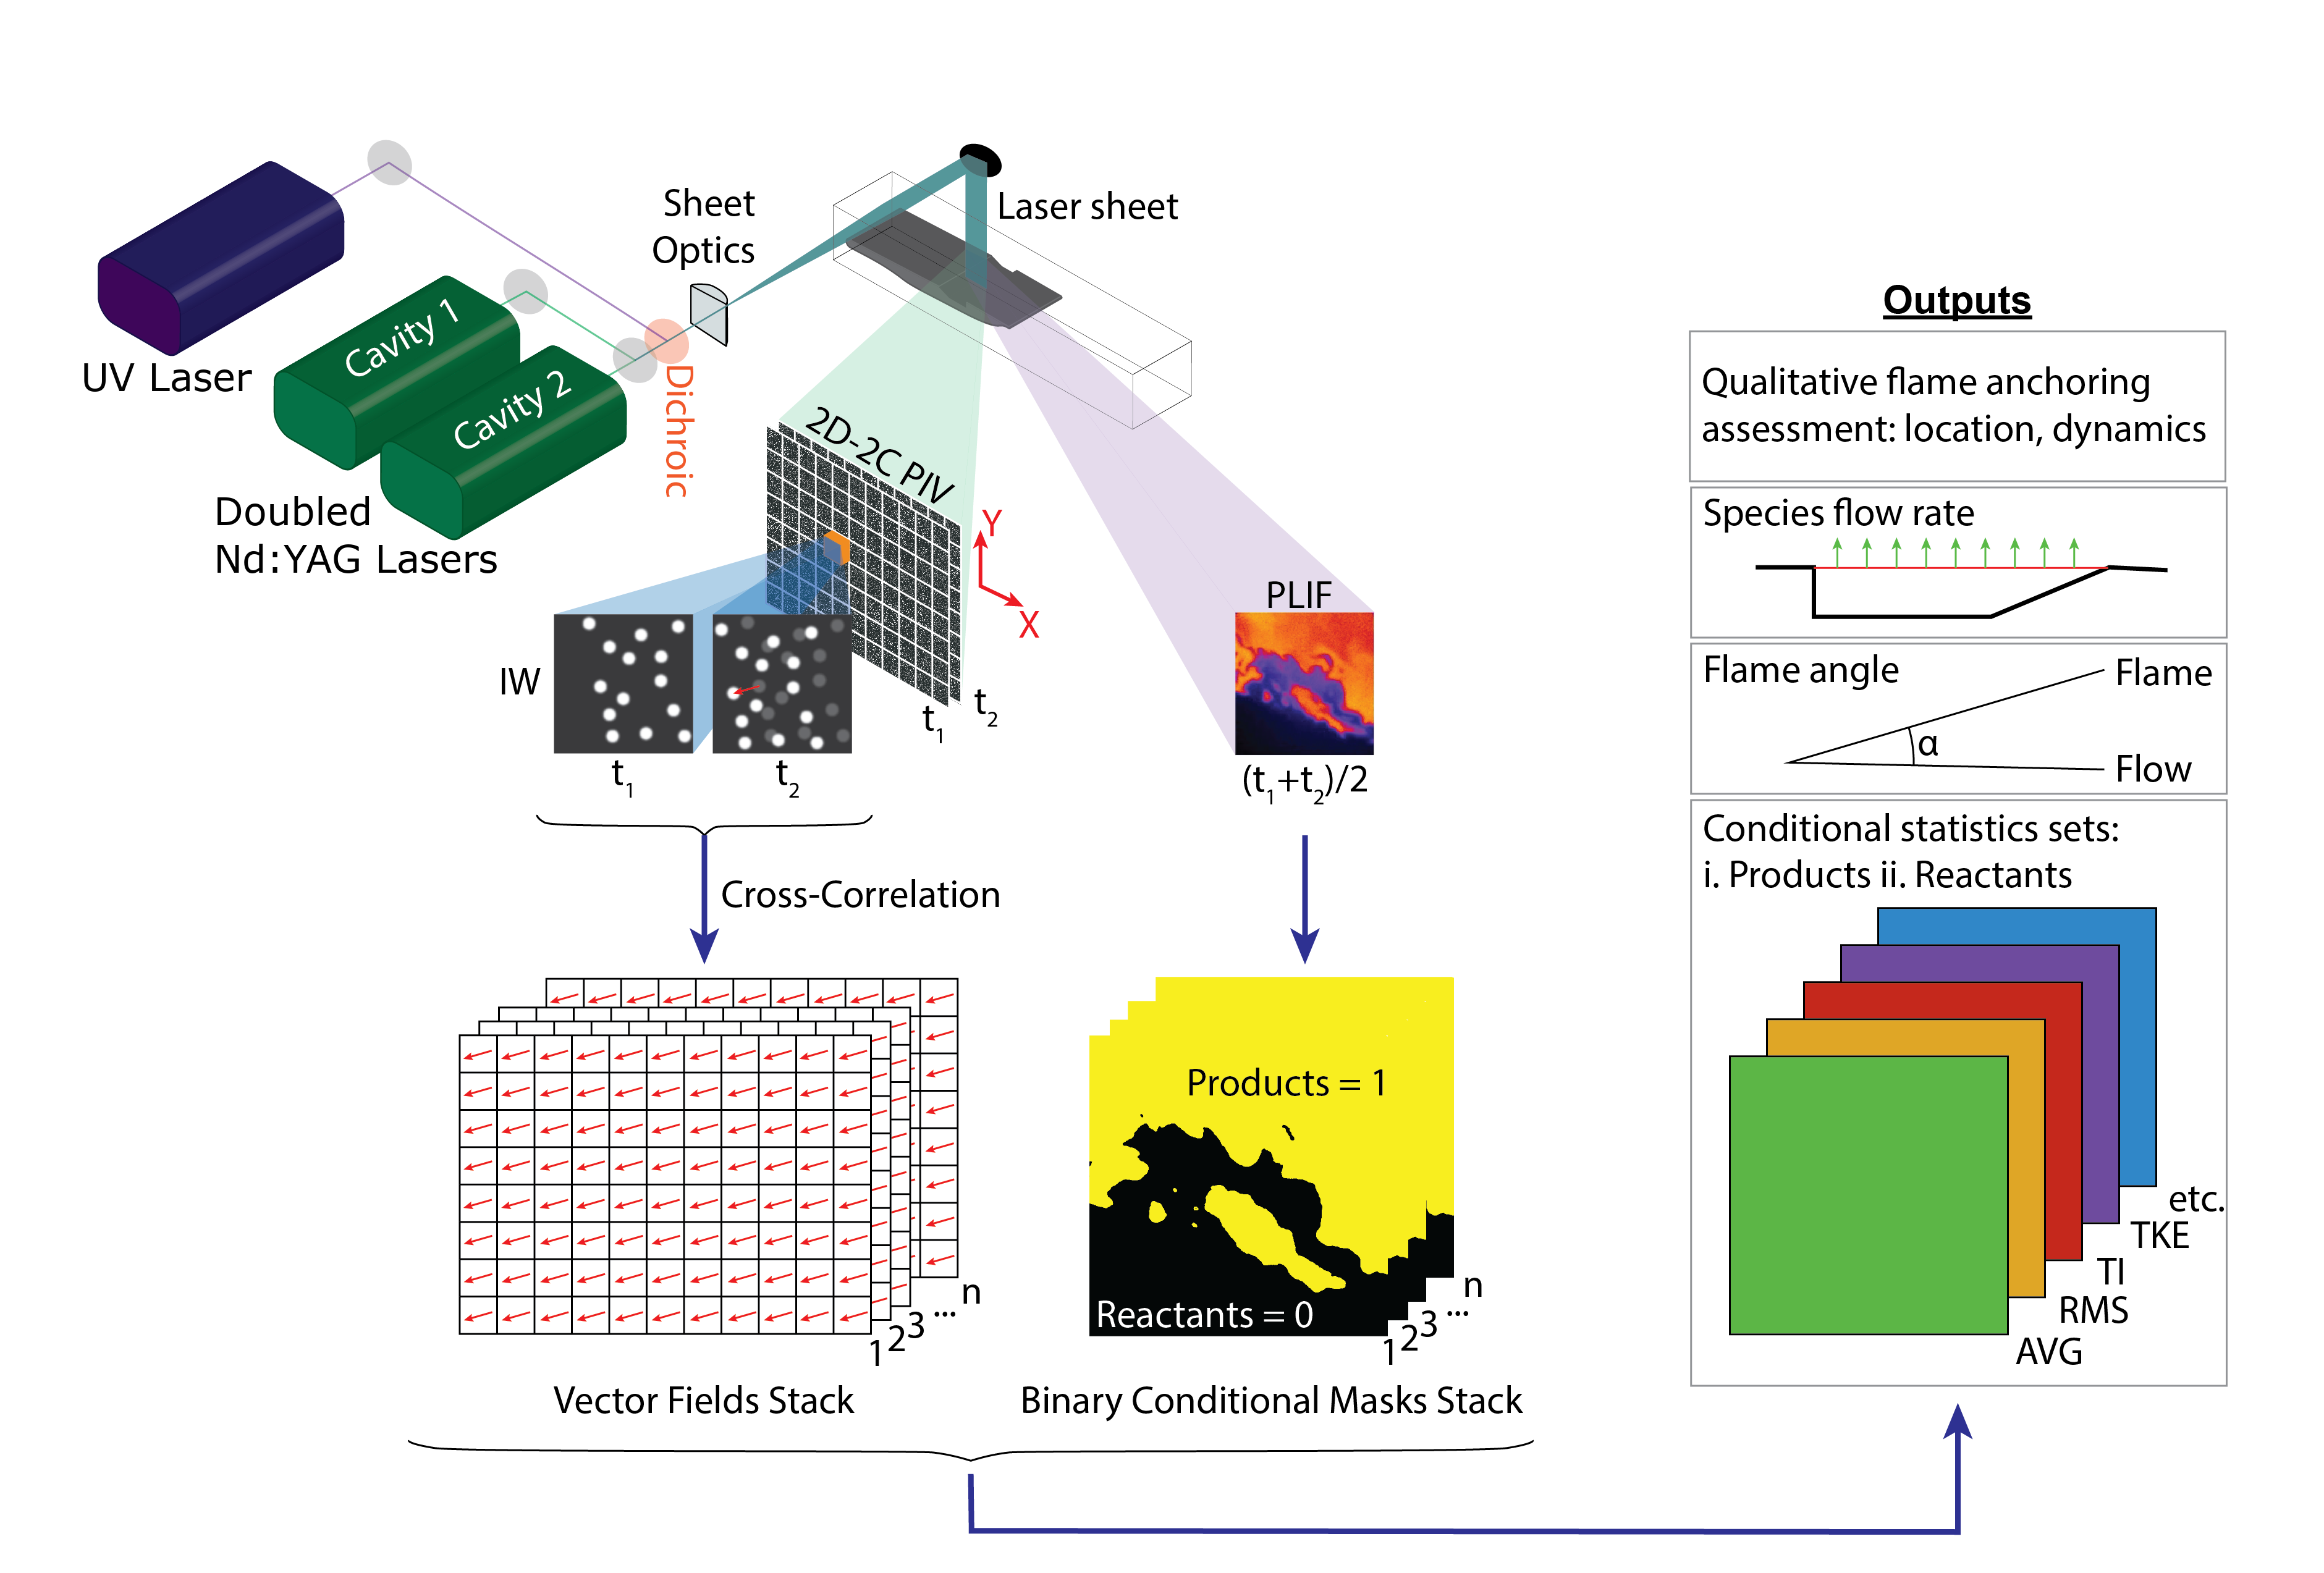
\includegraphics[width=6.5in, trim=0.6in 0in 0.7in 0in, clip]{figures/PIV-PLIFsetup/PIV-PLIFArtboard1@3x.png} %pdfcrop
\caption{Principle of the combined PIV-PLIF technique. AVG: average; RMS: Root-Mean-Square; TI: Turbulence Intensity; TKE: Turbulent Kinetic Energy.}\label{fig:ch3_method_setup}
\end{figure*}

\begin{figure}
\centering
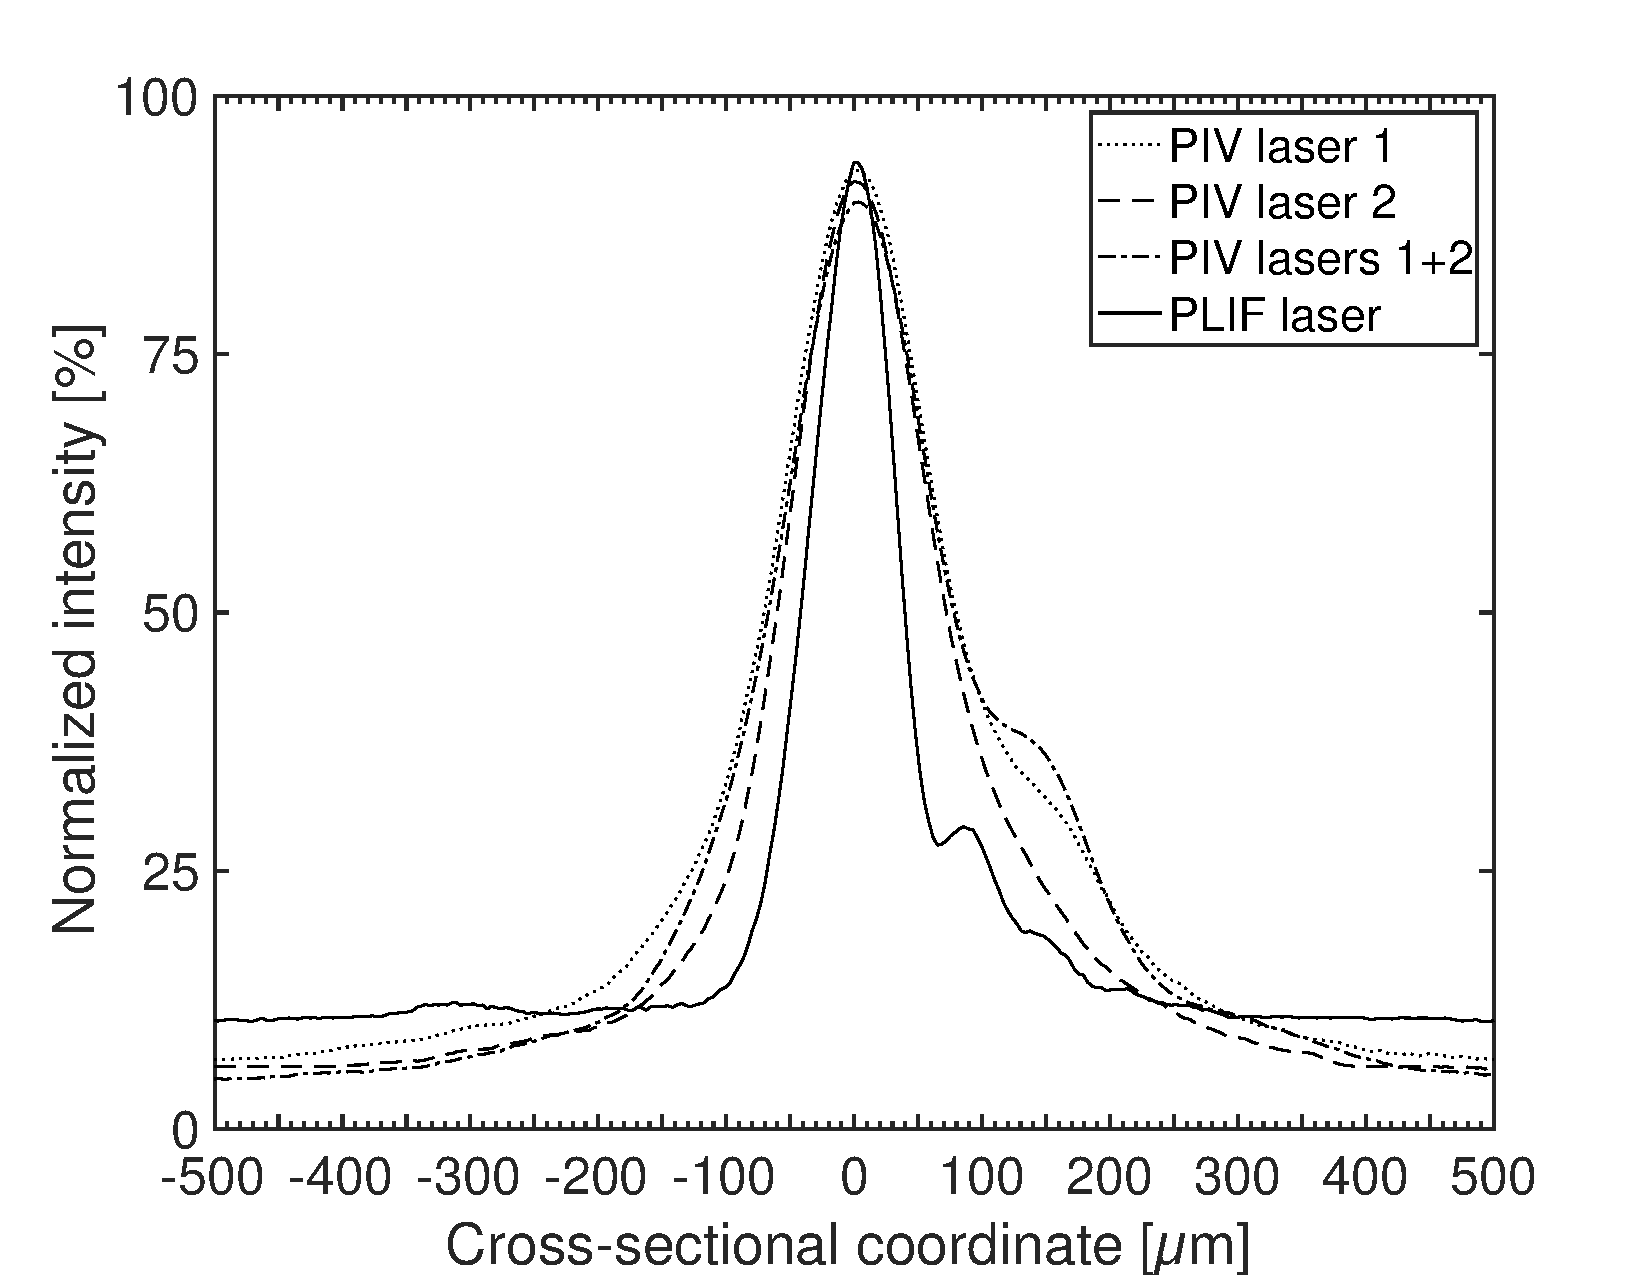
\includegraphics[width=3.25in, trim=0.35in 0in 0.75in 0in, clip]{figures/B_f_overlap_all} %pdfcrop
\caption{Cross-sectional intensity profiles of laser sheets.}\label{fig:ch3_meas_LS_thick}
\end{figure}

The PIV and PLIF cameras are mounted together on a three-axis translational stage system, allowing the field of view to be moved during tunnel operation.
The PIV camera is a 14-bits, $1600\times 1200$ pixel LaVision Imager Pro X 2M. The camera is angled by 4 degrees about the tunnel $x$ axis to mask laser reflections off the wall. A Scheimpflug lens adapter adjusts the focal plane back onto the laser sheet. The camera is mounted with a Micro-Nikkor 105mm f/2.8 lens at a magnification $m=1:1.8$ and an f-number of 11, and a $532 \pm 10$ nm-wide bandpass filter. The lens magnification corresponds to the maximum allowed by the setup constraints; the PIV lens and the PLIF lens would conflict with each other at any higher magnification. The PLIF PI-Max 4 camera is equipped with a 100 mm focal length Cerco lens and a Scheimpflug angle adapter. It captures $512\times 512$ pixel images after $2\times2$ pixel binning. A Semrock FF02-320/40- 30-D bandpass filter reflected light outside the 310-340 nm range \citep{GeipelRockwellChelliahEtAl2017}. 

The PLIF camera is angled by approximately 30 degrees about the tunnel $y$ axis to image the same field of view as the PIV camera. Due to the viewing angle, the region near the cavity ramp is shadowed to the PLIF camera. In addition, the FOV is shifted slightly downstream of the cavity leading edge to avoid imaging laser reflections with the PIV camera, causing clipping of the region immediately behind the cavity backward-facing step. The imaging systems are calibrated simultaneously using a grid with $250~ \mathrm{\upmu m}$ dot spacing. FOV overlap is performed by dewarping and scaling the grid images from both systems before overlapping a spatial marker and all dots across the images. The overlap accuracy is estimated on the order of $10~ \mathrm{\upmu m}$. 

Particle image velocimetry in combusting flows faces challenges that include temperatures greater than 2000 K, wide-spectrum radiation from the flame, and strong gradients in thermo-fluid dynamic variables \citep{StellaGujKompenhansEtAl2001}. This is compounded with the facility high-enthalpy flow, causing the commonly-used PIV tracer materials (e.g. oxides of aluminum, titanium, and silicon ($\mathrm{Al_2O_3}$, $\mathrm{TiO_2}$, $\mathrm{SiO_2}$, \citep{Melling1997, FangHong2018}) to adhere to the facility windows. This adherence quickly prevents flow visualization. 
Kirik et al. \cite{KirikGoyneMcDanielEtAl2017} introduced the use of graphite nano-flakes as tracer particles for the PIV of a cavity flameholder. These $1.1~ \mathrm{\upmu m}$-long and $16~ \mathrm{nm}$-thick flakes have an estimated Stokes number of $St\sim 0.05$ \cite{KirikGoyneMcDanielEtAl2015} corresponding to RMS velocity errors of less than 1\% \citep{SamimyLele1991}. 
Graphite particles prevent window fouling because they do not adhere to the windows as readily. 
Seeding of the graphite nanoflake tracer particles for PIV \citep{KirikGoyneMcDanielEtAl2015} is performed with a fluidized bed seeder \citep{HowisonGoyne2010}. The particles are injected upstream in the isolator, before the fuel injectors and on the centerline. The tracer particles are diffused across the cavity-side streamtube. 

\subsection*{Data processing}
Methodology for PIV processing is presented first, followed by PLIF processing methodology. The graphite nanoflakes used as PIV tracers have a low, angle-dependent reflectance causing poor signal-to-noise ratios. A novel approach solves this problem by pre-processing the images with a Logarithm Contrast-Stretch (LCS) transform, described in \cite{LieberThesis}, in order to compress the upper dynamic range relative to the lower dynamic range. The LCS pre-processing filter increases cross-correlation signal-to-noise ratio in the presence of strong particle image intensity changes between frames. 
The cross-correlation signal-to-noise ratio is also significantly affected by the flame luminosity. Chemiluminescence from the ethylene flame passes through the camera bandpass filter to reach values of 800-8,000 pixel counts depending on the seeding density. This disturbance is particularly severe in the second frame which is constrained by design to a longer exposure time of up to tens of milliseconds depending on the first frame read-out time. A moving average filter across 20 images is thus applied and each frame normalized by the corresponding average before the LCS filter is applied. Lens flares from strong laser reflections off the facility walls are masked before reaching the camera lens.

The data set is then processed with the LaVision DaVis 8.4 cross-correlation algorithm. 
Instantaneous velocities are computed using multi-pass deformed interrogation windows down to 48 $\times$ 48 pixels, corresponding to a velocimetry resolution of $643~ \mathrm{\upmu m}$. Median filters, correlation value thresholds, and outliers detection from temporal distributions remove spurious vectors. Adequate convergence in the velocity mean and RMS is ensured with sample sizes of 1,000 vectors or more. The turbulent kinetic energy (TKE) is estimated by taking the third RMS component as the average of the streamwise and transverse components. The actual three-components turbulent intensity (TI) is on the order of 1\% greater while the TKE is on the order of 100 $\mathrm{m^2/s^2}$ smaller according to a parallel LES study by \cite{Nielsen2019}).
Uncertainties are computed for each instantaneous velocity vector using the measurement signal with the correlation statistics method by \cite{Wieneke2015}, and hardware specifications as detailed in \cite{LieberThesis}. The RMS velocity is corrected by substracting random error fluctuations to isolate flow fluctuations only \citep{SciacchitanoWieneke2016}. 

Processing of the PLIF data is addressed next. The PLIF images are scaled down to $161~ \mathrm{\upmu m/pixel}$ and cropped to match the PIV vector spacing and PIV coordinates. The spatial and temporal resolutions of the PIV measurements are respectively one and five orders of magnitude lower than the estimated Kolmogorov length and time scales. While turbulence spectrum clipping in high $Re$ flows remains inevitable with current technological capabilities, this effect is mitigated for the investigation of turbulence-chemistry interactions: Poinsot et al. \cite{PoinsotVeynanteCandel1991} noted that eddies smaller than the order of the flame front thickness do not quench the flame due to viscous dissipation prior to the flame front. Previous work also demonstrated the dominance of large scale structures in governing the cavity-stabilized combustion process \citep{XavierVandelGodardEtAl2016}. 
The current PLIF technique can only provide qualitative measurements indicative of relative OH concentrations. It is however useful for separating flow regions into reactants- and products-preponderant domains and identifying the location of the flame front \citep{CantuGalloCutlerEtAl2016a}.  An image processing algorithm has been developed to accurately contour the reactants domain; details may be found in \citet{Geipel2019}. 
The image is binarized with one indicating combustion products and zero indicating reactants.  
The binarized PLIF images can be used with the corresponding instantaneous velocities field to output velocities conditioned on both combustion products and reactants (Fig. \ref{fig:ch3_method_setup}). Statistics are finally extracted from the two stacks of velocity fields. The mean transverse velocities across a straight line at $y/H=0$ between the cavity leading and trailing edges, i.e. $x/H=0$ and $x/H=6$, is taken as a representation of the species flux out of the cavity. Mean transverse velocities are similarly estimated at the flame front. 

In the following figures, CLE refers to cavity leading edge. The surface of the tunnel wall opposite to the flameholder is represented by the continuous line at $y/H$ = 4.8 and the insert containing the cavity is shown in grey. A sub-sample of average velocity vectors are displayed with white arrows to show flow directionality. Streamlines in purple originate from each vector.
The flame intermittency is the fraction of instantaneous PLIF measurements in which a significant amount of OH is present at a given location. Intermittency maps are shown as overlayed white contours at the 25\%, 50\%, 75\% and 100\% intermittency levels.


\section*{Statistical results}
Statistical results describe the key flow features, flame topology, and fluctuations over an ensemble of measurements. The mean and fluctuating statistics on the velocimetry presented below are first correlated with the mean PLIF signal. Mean conditional velocities are computed based on the instantaneous presence or absence of OH; this provides independent velocity means for products and reactants. As will be discussed below, independent PIV and PLIF statistics agree well with previous studies with separate acquisitions \citep{TuttleCarterHsu2014, Kirik2017} while new insights about cavity dynamics are gained from the combined nature of the measurements.

\subsection*{Mean velocities}
The streamwise axial mean velocity component is displayed in Fig. \ref{fig:B1_Ux_AVG}. Throughout Fig. \ref{fig:ch3_UxAVG_PIVPLIF} and similar figures, the horizontal white line near $y/H=5$ denotes the duct wall opposite the cavity. Uncertainties for a 95\% interval are in the range $\pm2$ to 7 m/s. The duct flow velocimetry above the cavity ($y/H>0$) is very similar in trends and values to velocimetry at the inflow to the cavity \citep{LieberThesis}, characterized by the opposite-wall boundary layer that spans most of the duct height. This boundary layer merges with the thin shear layer created at the cavity leading edge; the peak axial mean velocity of 360 m/s is located near $y/H = 0.75$ and drops to 100 to 200 m/s at $y/H=0$. Fig. \ref{fig:B1_Uy_AVG} displays the transverse mean velocities map;  uncertainties are in the range $\pm1$ to 3 m/s. Transverse means are negative in the main duct flow on the order of 1 m/s and become zero or positive in the vicinity of the cavity between $y/H =$ 1.5 to 0.5. They sharply drop into negative values in the shear layer. Along the shear layer, transverse velocities remain negative and further decrease with increasing distance from the CLE, with the exception of the region nearest to the CLE where transverse velocities are slightly positive. The $y$-location of zero transverse velocity and the $y$-location of the maximum gradient in axial velocities is raised above the cavity interface as the flow goes further downstream. This indicates a broadened or lifted shear layer starting near $x/H=3$. The shear layer impinges on average onto the cavity ramp, forming a closed cavity flow as observed for larger geometries \citep{Kirik2017}. 

The mean velocities within the cavity are characterized by flow recirculation. The cavity axial velocities are in the range $\pm 50$ m/s (Fig. \ref{fig:B1_Ux_AVG}) and the transverse velocities $\pm 30$ m/s (Fig. \ref{fig:B1_Uy_AVG}). Streamlines in Fig. \ref{fig:B1_PLIF} highlight an elliptical recirculation region with a major axis intersecting with the CLE and a point on the ramp located at $y/H=-0.75$ and $x/H=4.25$. This axis coincides with the directionality of PLIF contours in this region. In addition, the center of the ellipse, located at $y/H=-0.$ and $x/H=2.5$, coincides with the region of constant flameholding indicated by 100\% flame intermittency. Thus mixing and combustion occurs in the first half of the elliptical recirculation zone, from the CLE side to the ramp side, and the second half re-circulates a constantly-present pool of combustion products and radicals. As will be discussed later in this paper, instantaneous measurements reveal that two large recirculation eddies are present in the cavity; the combination of two translating clockwise-rotating eddies lead to the observed elliptical streamlines when averaged over time.

The distribution of the number of good velocity measurements in each 48 $\times$ 48 pixel interrogation window out of a data set of 2000 PIV images (see the contours in Fig. \ref{fig:B1_PLIF2}) shows correlation with the flame intermittency. Regions of high intermittency have lower PIV vector counts and vice-versa. This trend can be explained by the reduction in gas and particle density arising from an increase in temperature and perhaps also in part by combustion of particles. This correlation would tend to bias velocity statistics (mean, standard deviation, etc.) towards values for the reactants in regions of mixed products and reactants.  Such a bias will not occur where either reactants or products are present at all times (intermittency of 0 or 1). The ratio of the number of good velocity measurements in the products to the total number of good velocity measurements is compared to the intermittency in Fig. \ref{fig:B1_relative_sample_size}; since this ratio closely follows the flame intermittency, the level of bias is expected to be low. This analysis illustrates the usefulness of combined PIV-PLIF measurements in assessing the possibility of bias in the velocity statistics.

\begin{figure}
\centering
\subcaptionbox{Axial mean velocities.\label{fig:B1_Ux_AVG}}
         {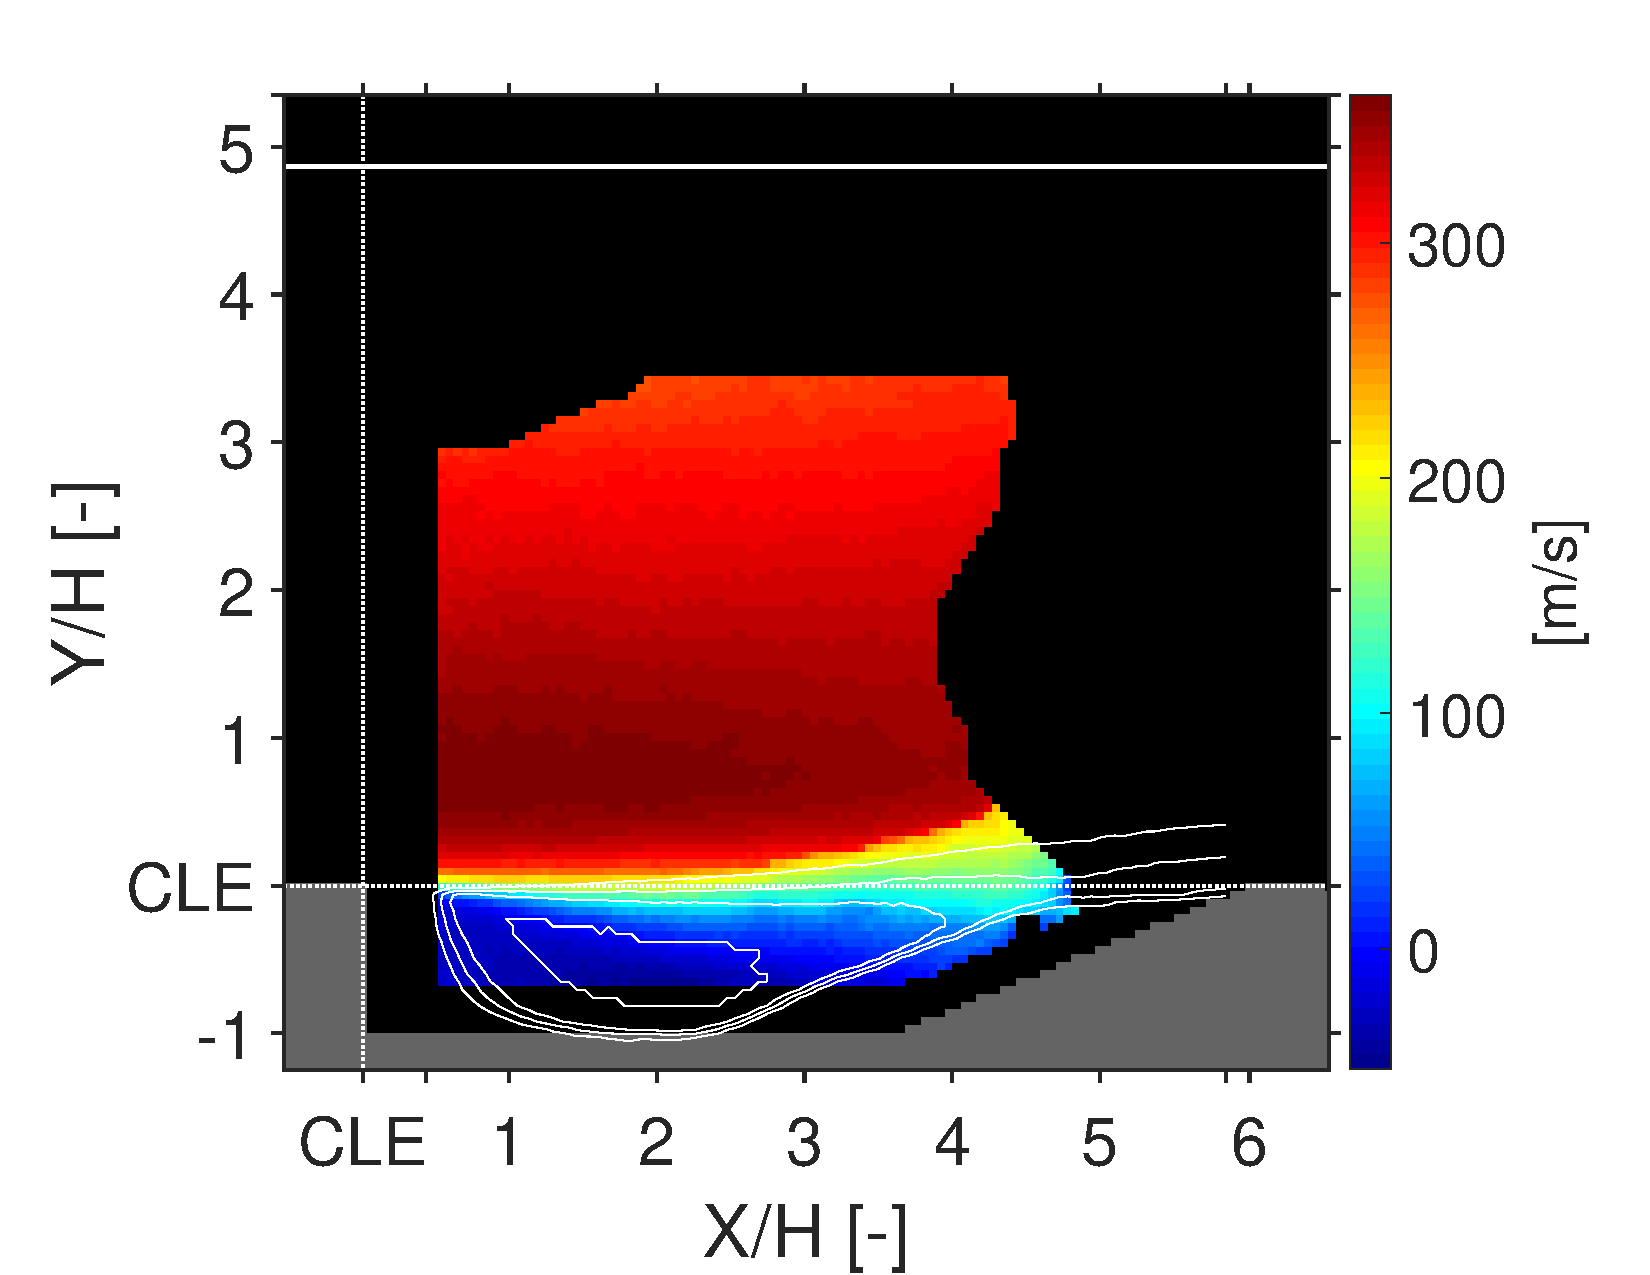
\includegraphics[width=3in,trim=0.35in 0 0.42in 0, clip]{figures/B1/whole_statistics/B1_Ux_AVG}}
         \hspace{0.4in}
\subcaptionbox{Transverse mean velocities.\label{fig:B1_Uy_AVG}}
         {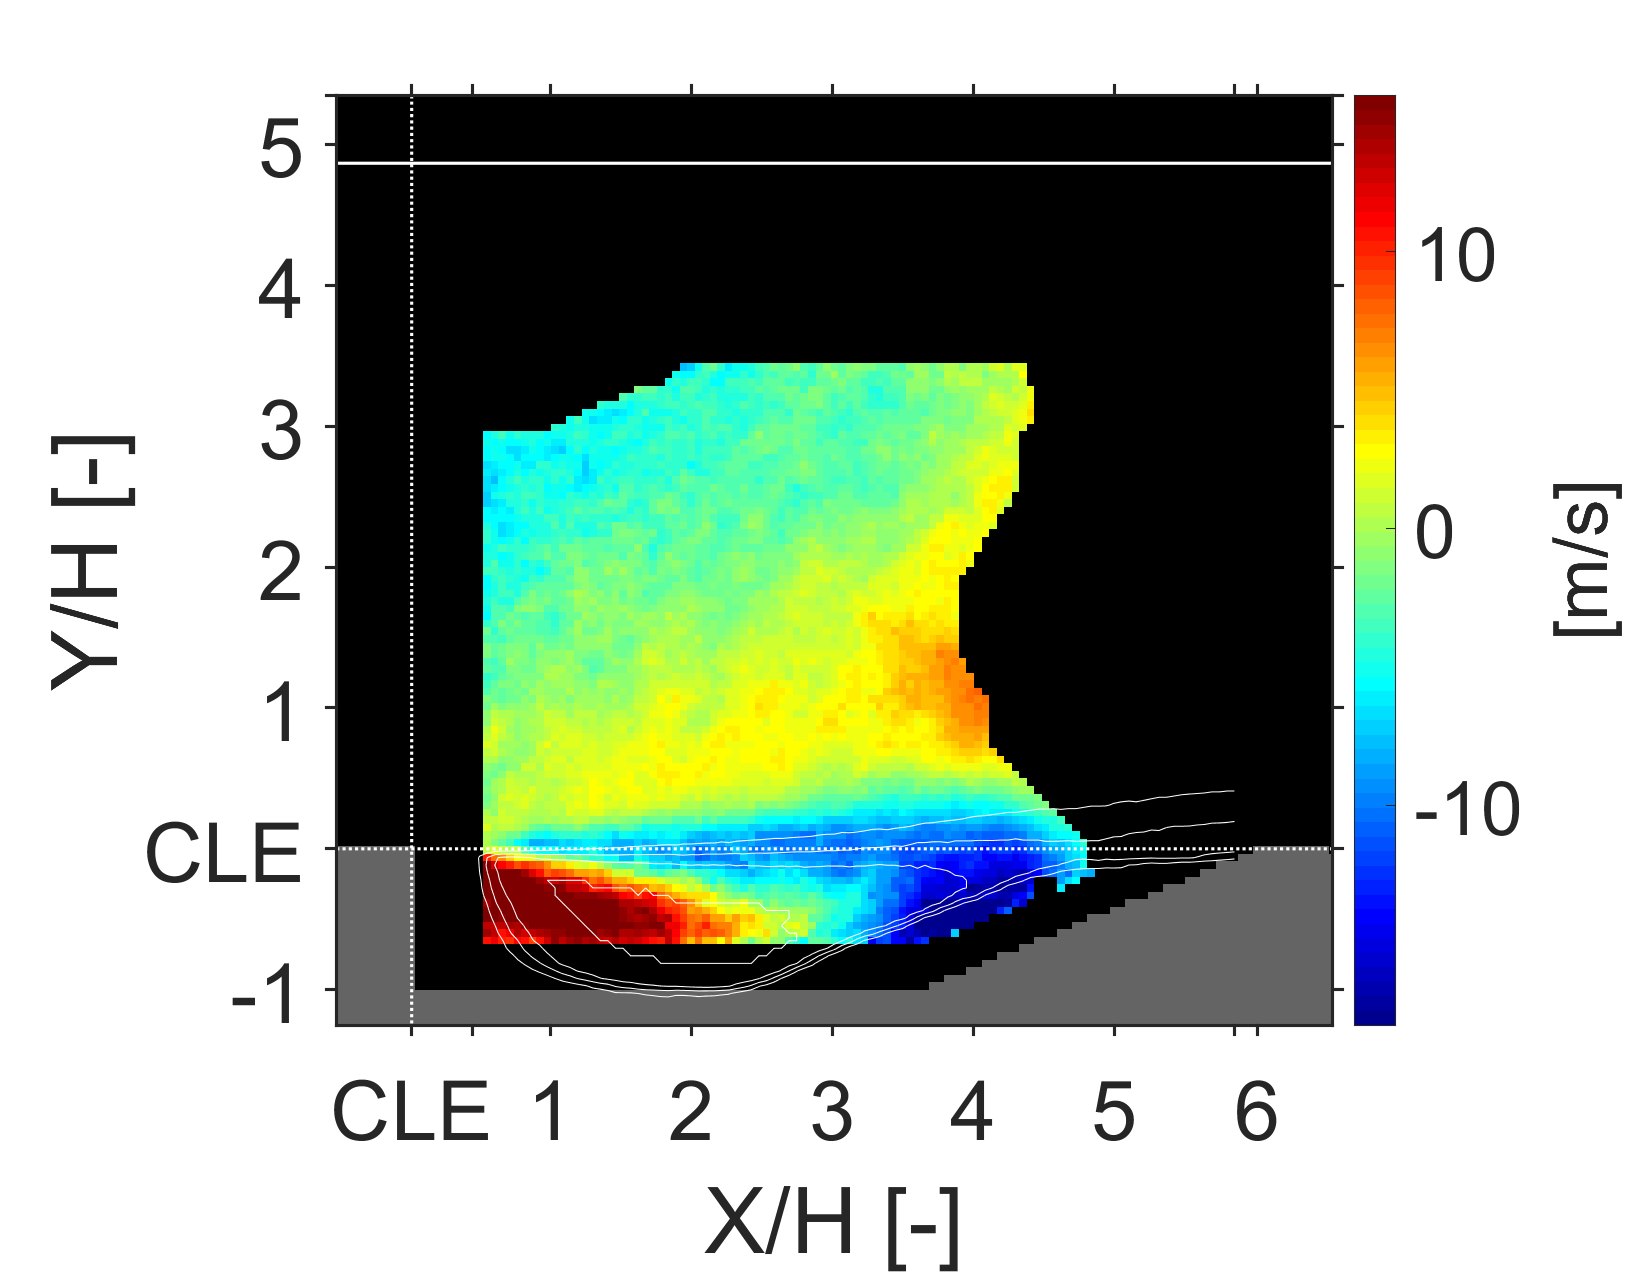
\includegraphics[width=3in,trim=0.35in 0 0.42in 0, clip]{figures/B1/whole_statistics/B1_Uy_AVG}}
         \newline
        \subcaptionbox{Mean OH-PLIF signal overlayed with select PIV vectors and streamlines.\label{fig:B1_PLIF}}
{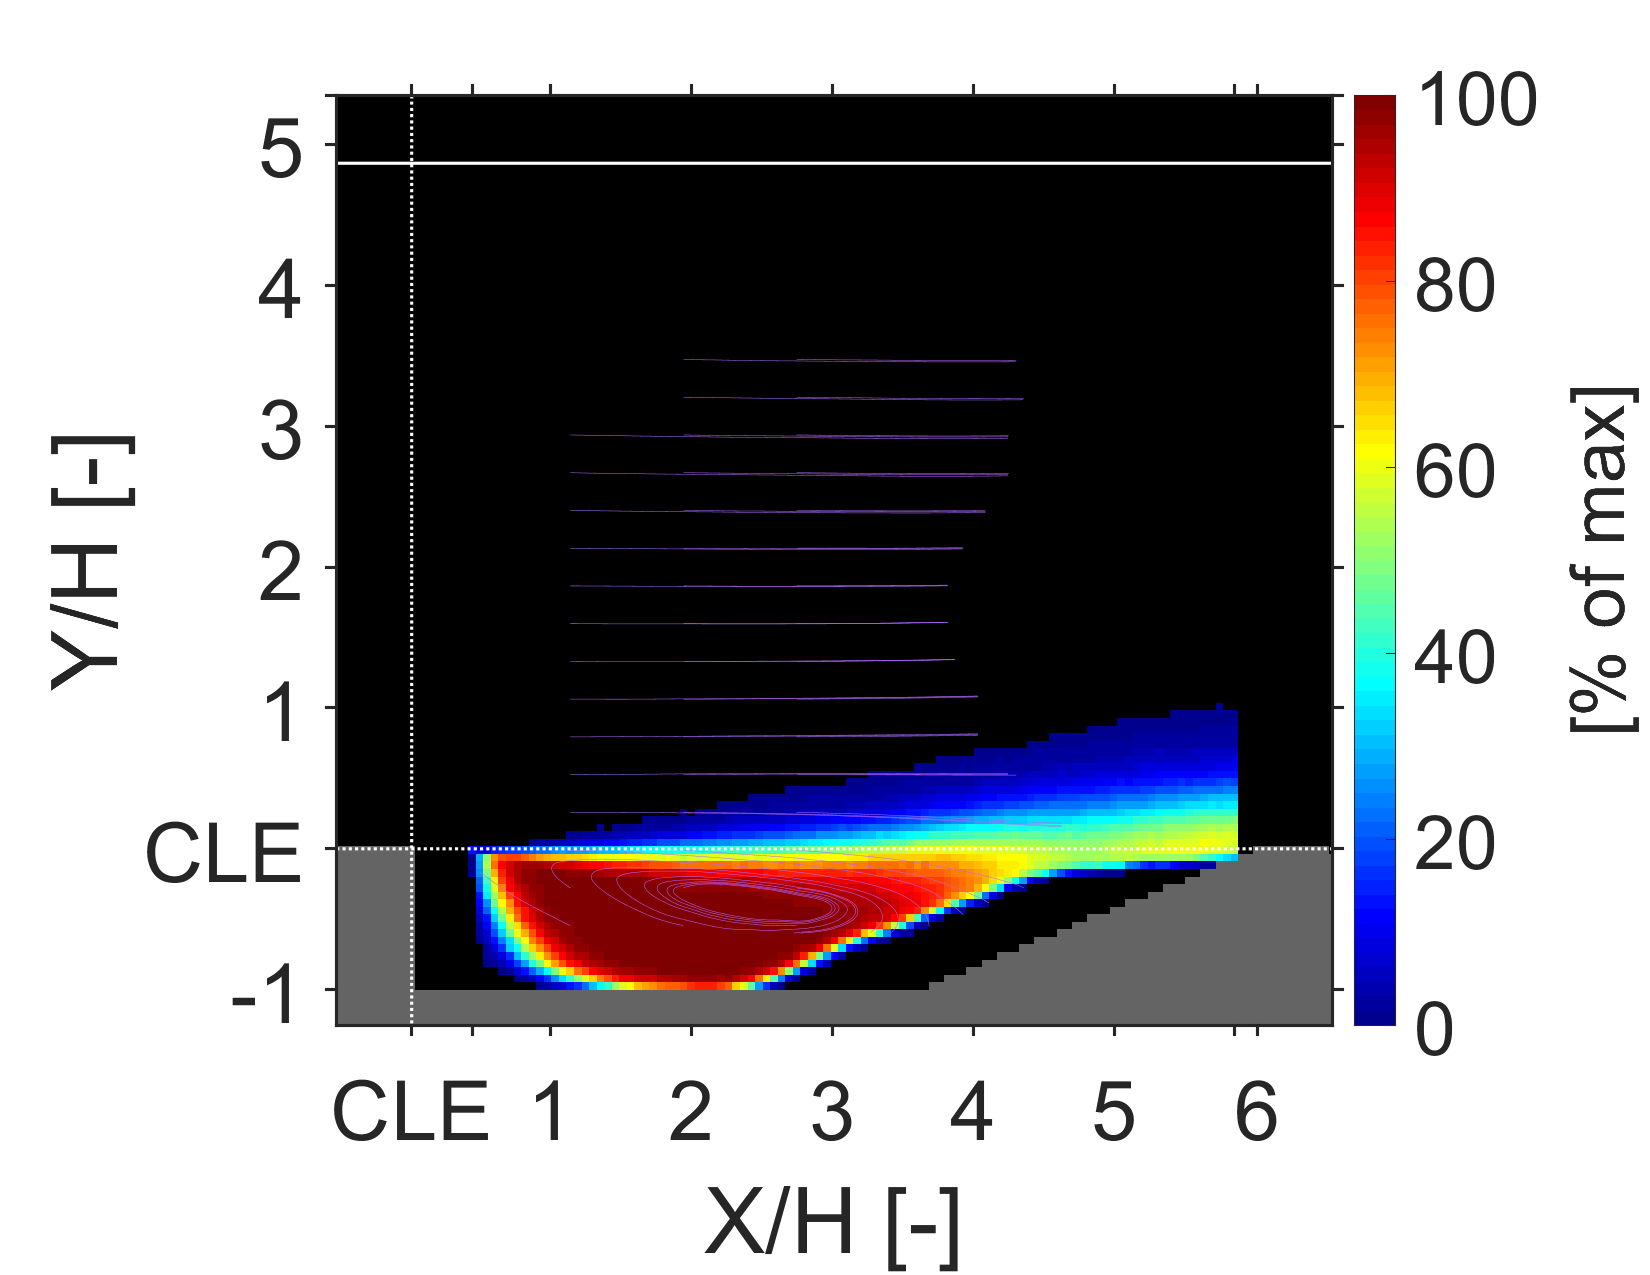
\includegraphics[width=3in,trim=0.35in 0 0.42in 0, clip]{figures/B1/whole_statistics/B1_PLIF}}
         \hspace{0.4in}
\subcaptionbox{Number of good velocity measurements per interrogation window.\label{fig:B1_PLIF2}}
{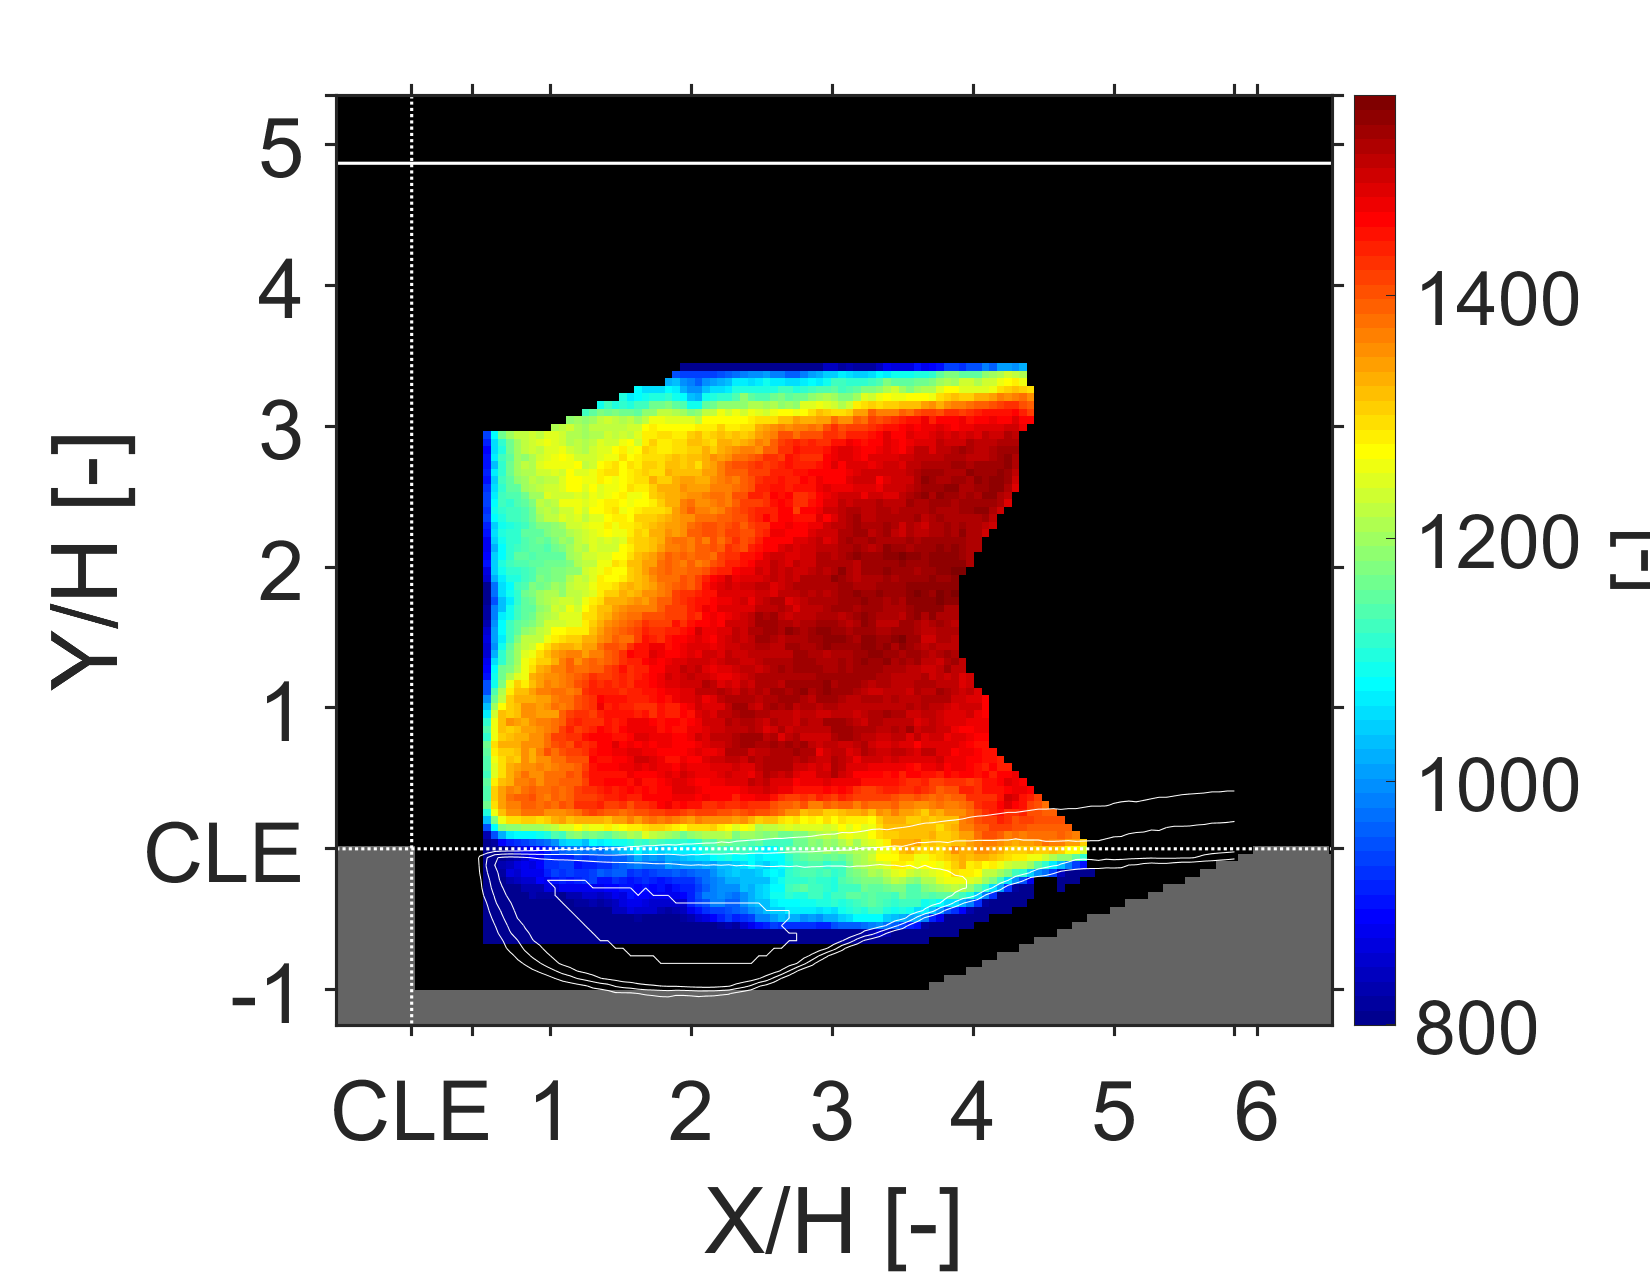
\includegraphics[width=3in,trim=0.35in 0 0.2in 0, clip]{figures/B1/whole_statistics/B1_sample_size}}
\newline
        \subcaptionbox{Fraction of good velocity measurements that are in the products.\label{fig:B1_relative_sample_size}}
{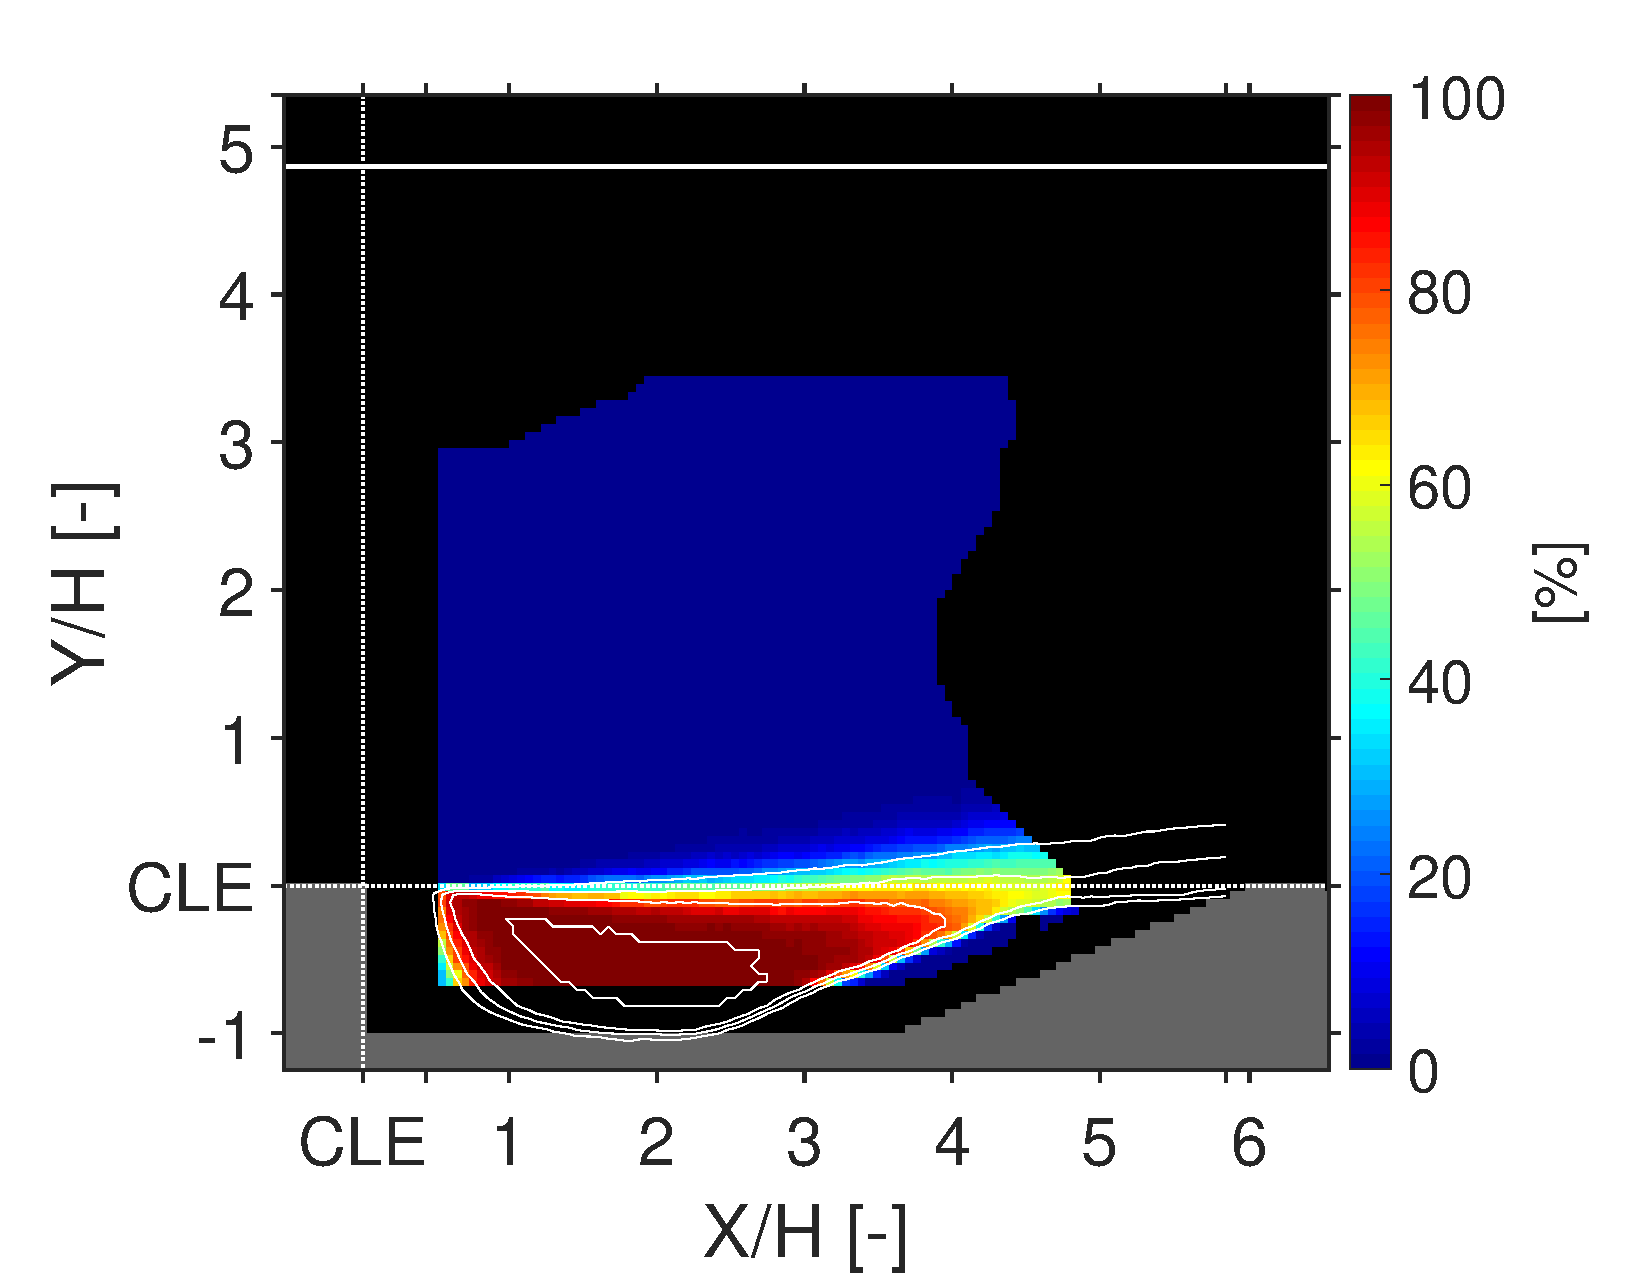
\includegraphics[width=3in,trim=0.35in 0 0.42in 0, clip]{figures/B1/cond_statistics/B1_relative_sample_size}}
\caption{Mean velocity fields with flame intermittency contours}\label{fig:ch3_UxAVG_PIVPLIF}
\end{figure}

\subsection*{Fluctuations}
Figure \ref{fig:ch3_UxRMS_PIVPLIF} displays the field of the velocity RMS, representative of flow fluctuations.  Uncertainties in the axial velocity for a 95$\%$ confidence interval are in the range $\pm5$ to 10$\%$ and for the transverse velocity are in the range $\pm6$ to 10 $\%$.  RMS values in the flow above the shear layer are similar to the inflow values measured at $x/H=-1.6$ presented in \cite{LieberThesis}. The axial and transverse fluctuations in the main duct flow increase towards the opposite wall due to the presence of the thick boundary layer. The main duct flow also shows turbulent anisotropy with $U_{y,~ RMS}$ in the range 30 to 35 m/s and $U_{x,~ RMS}$ in the range 50 to 55 m/s at $y/H=2.5$. 
The axial RMS velocity is highest in the shear layer and lowest in the upstream cavity corner. Peak values are found past $x/H=3$ above the cavity regions, hinting at disrupting product ejection events as observed in instantaneous PLIF measurements. 
A large region of heightened transverse RMS velocities coincides with the upper half of the elliptical recirculation region. Peak transverse RMS velocities occur on the ramp indicating shear layer impingement, in agreement with previous observations \citep{Kirik2017}. Similarly to the axial RMS, the transverse RMS drops in the cavity upstream corner where a small low-speed recirculation region was identified in a larger cavity \citep{Kirik2017}. Based on observations from \citet{Kirik2017}, this portion of the cavity is expected to be filled by hot, burned gases that are forced toward the front of the cavity by the recirculation process. These gases provide an ignition source for the fresh fuel-air mixture as they are entrained by the main recirculation zone into the cavity shear layer.

\begin{figure}
\centering
\subcaptionbox{Axial RMS velocities.\label{fig:B1_Ux_RMS}}
         {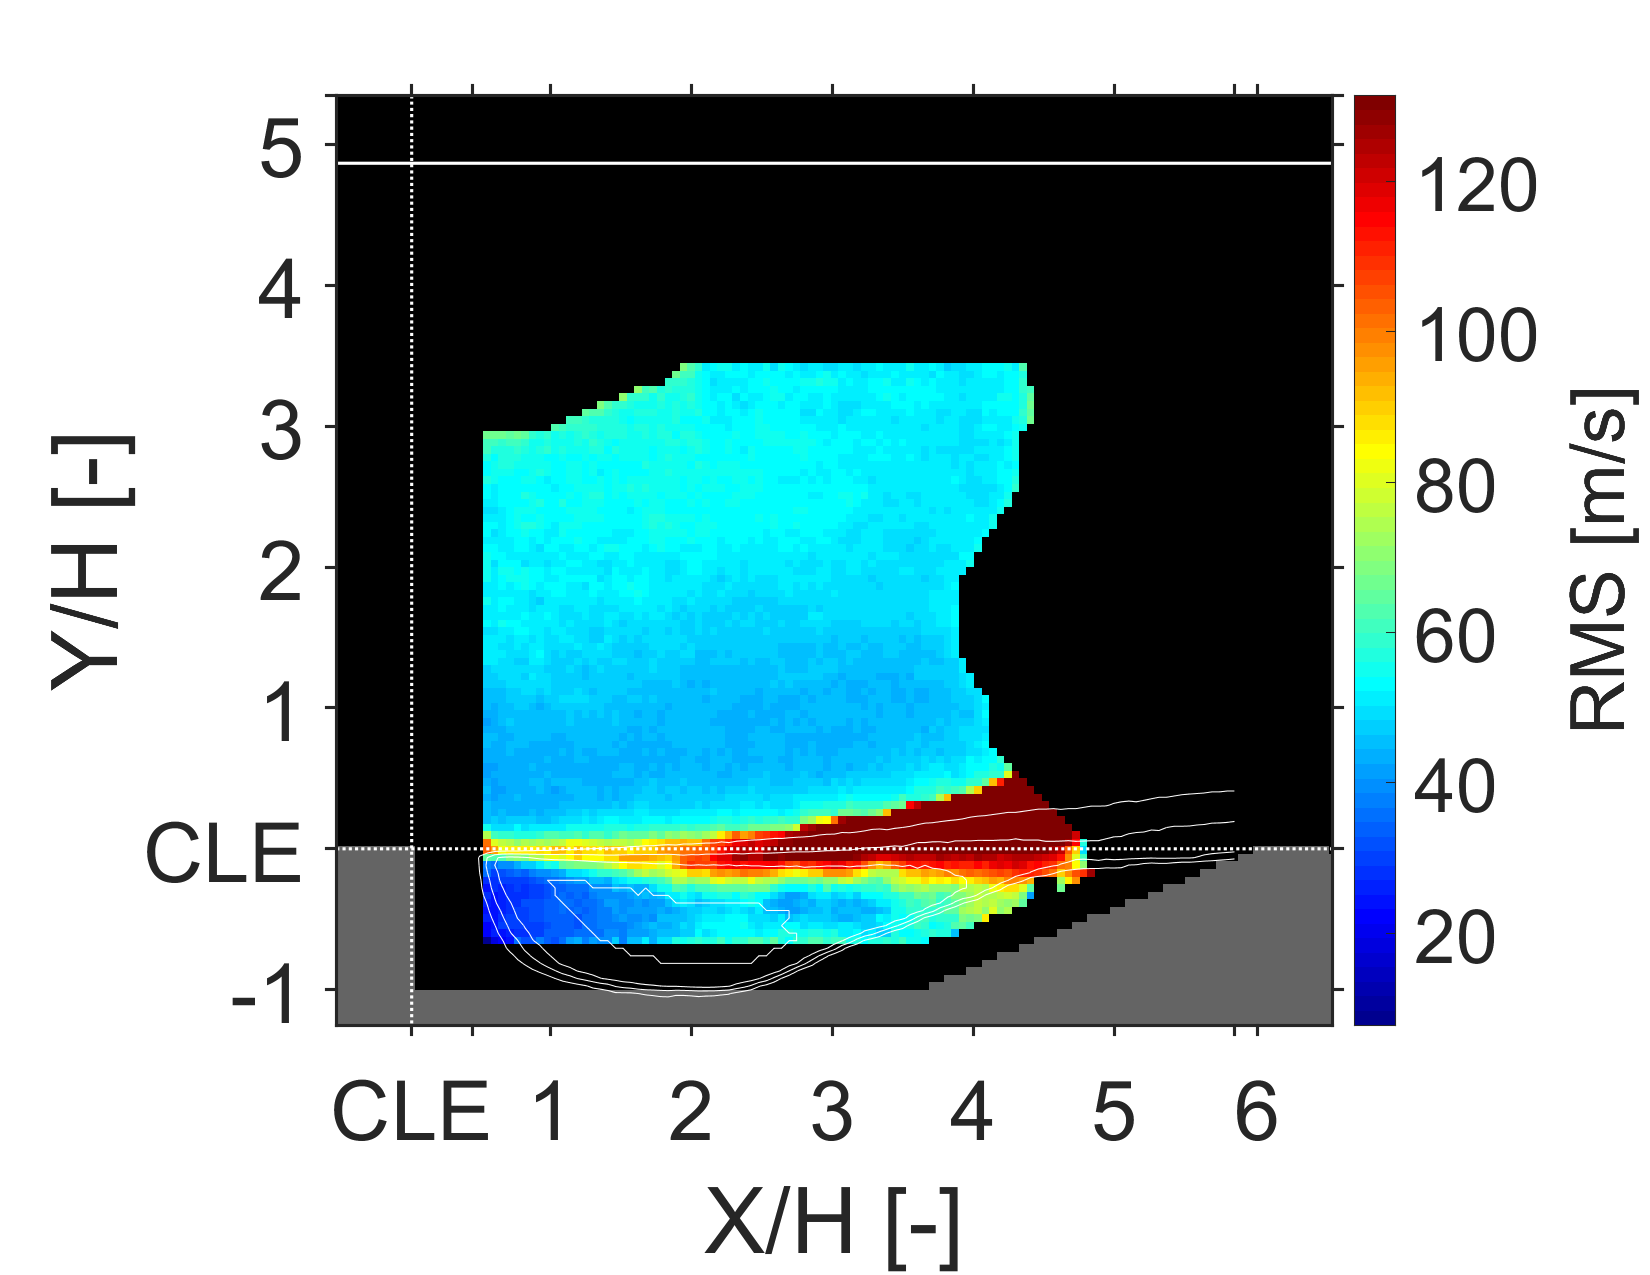
\includegraphics[width=3in,trim=0.35in 0 0.42in 0, clip]{figures/B1/whole_statistics/B1_Ux_RMS}}
        \hspace{0.4in}
\subcaptionbox{Transverse RMS velocities.\label{fig:B1_Uy_RMS}}
                {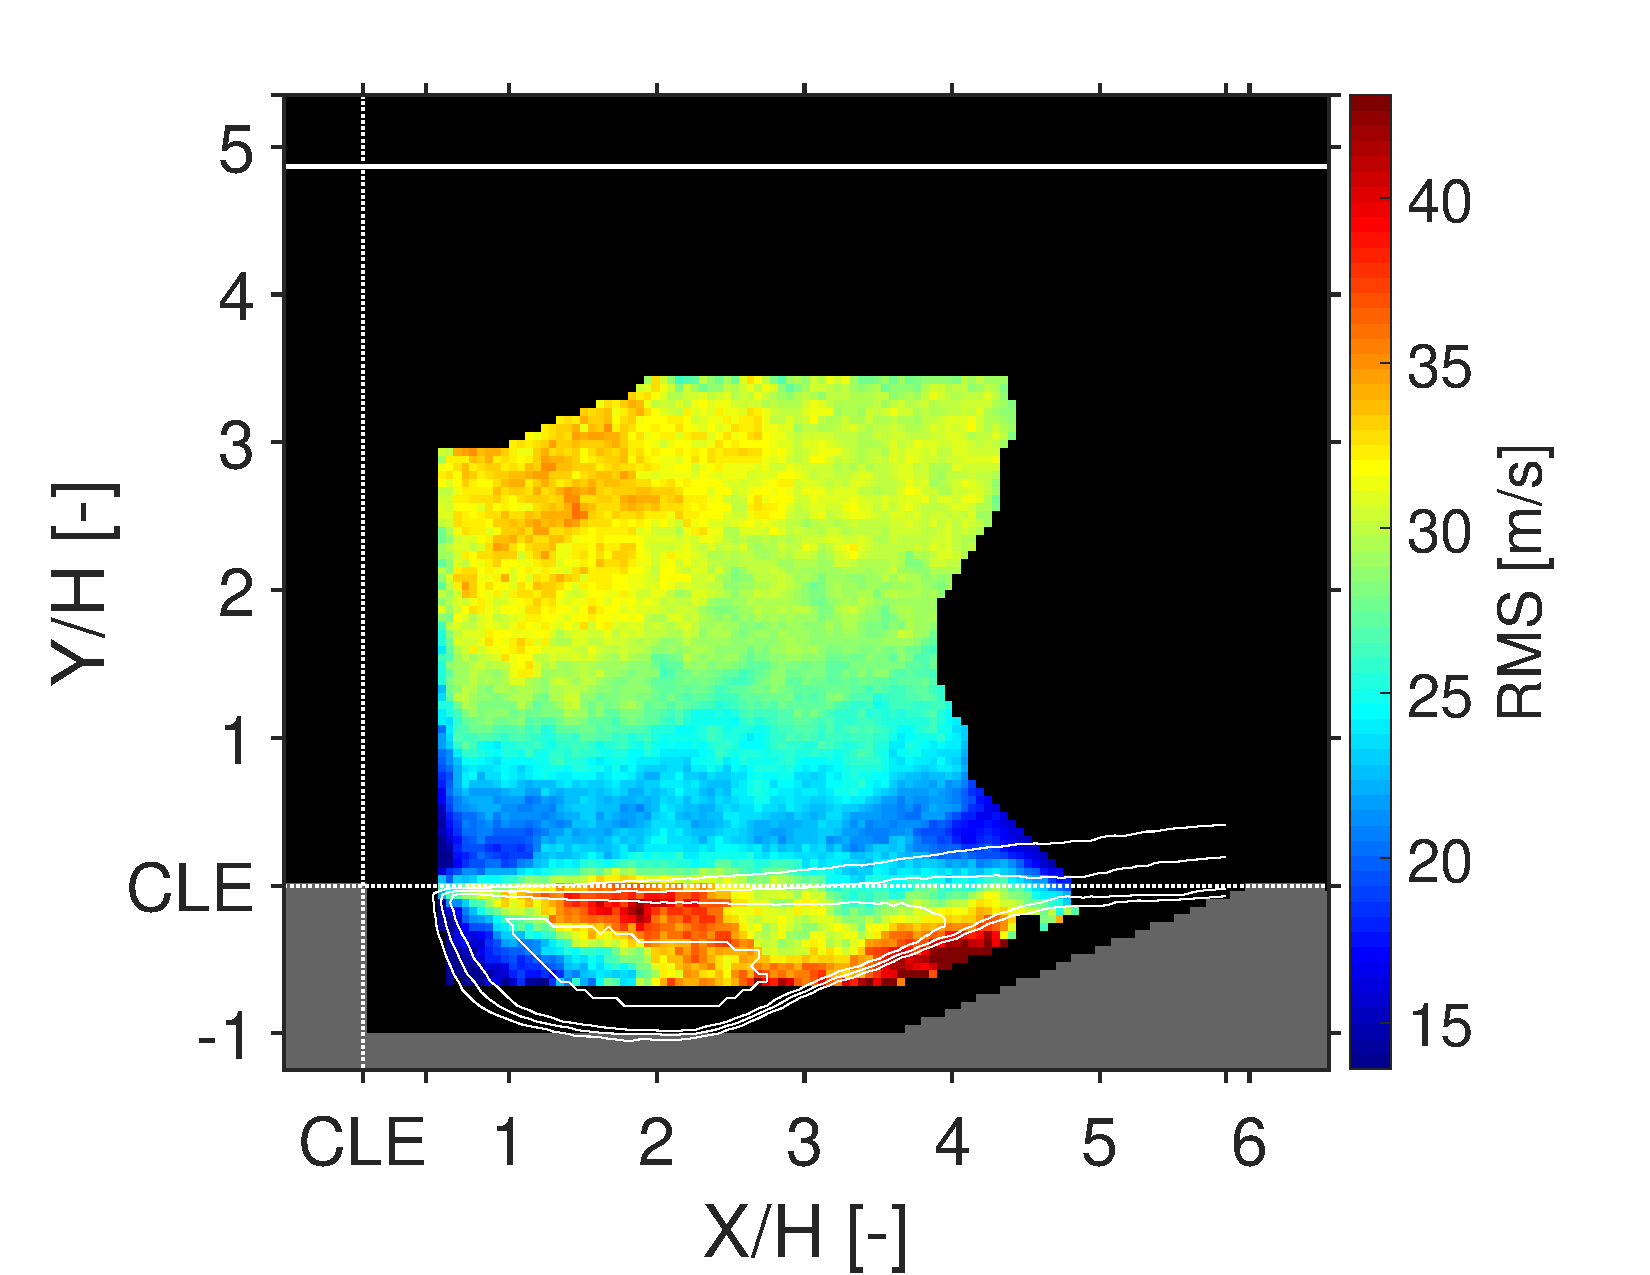
\includegraphics[width=3in,trim=0.35in 0 0.42in 0, clip]{figures/B1/whole_statistics/B1_Uy_RMS}}
\caption{RMS velocity components with flame intermittency contours}\label{fig:ch3_UxRMS_PIVPLIF}
\end{figure}

The turbulence intensity (Fig. \ref{fig:B1_Ux_TI}) displays a strong increase along the elliptical recirculation region major axis. Values exceeding 200$\%$ are detected in those areas, versus the main duct flow values of 10-15$\%$.  In contrast, the turbulent kinetic energy follows the trends of the axial fluctuations, i.e. with high values in the shear layer and a peak in the regions of product ejection. Uncertainties in the turbulence intensity are $\sim 4\%$ in duct flow and $<10\%$ in cavity (except on the elliptical recirculation zone axis).

\begin{figure}
\centering
\subcaptionbox{Turbulence intensities.\label{fig:B1_Ux_TI}}
        {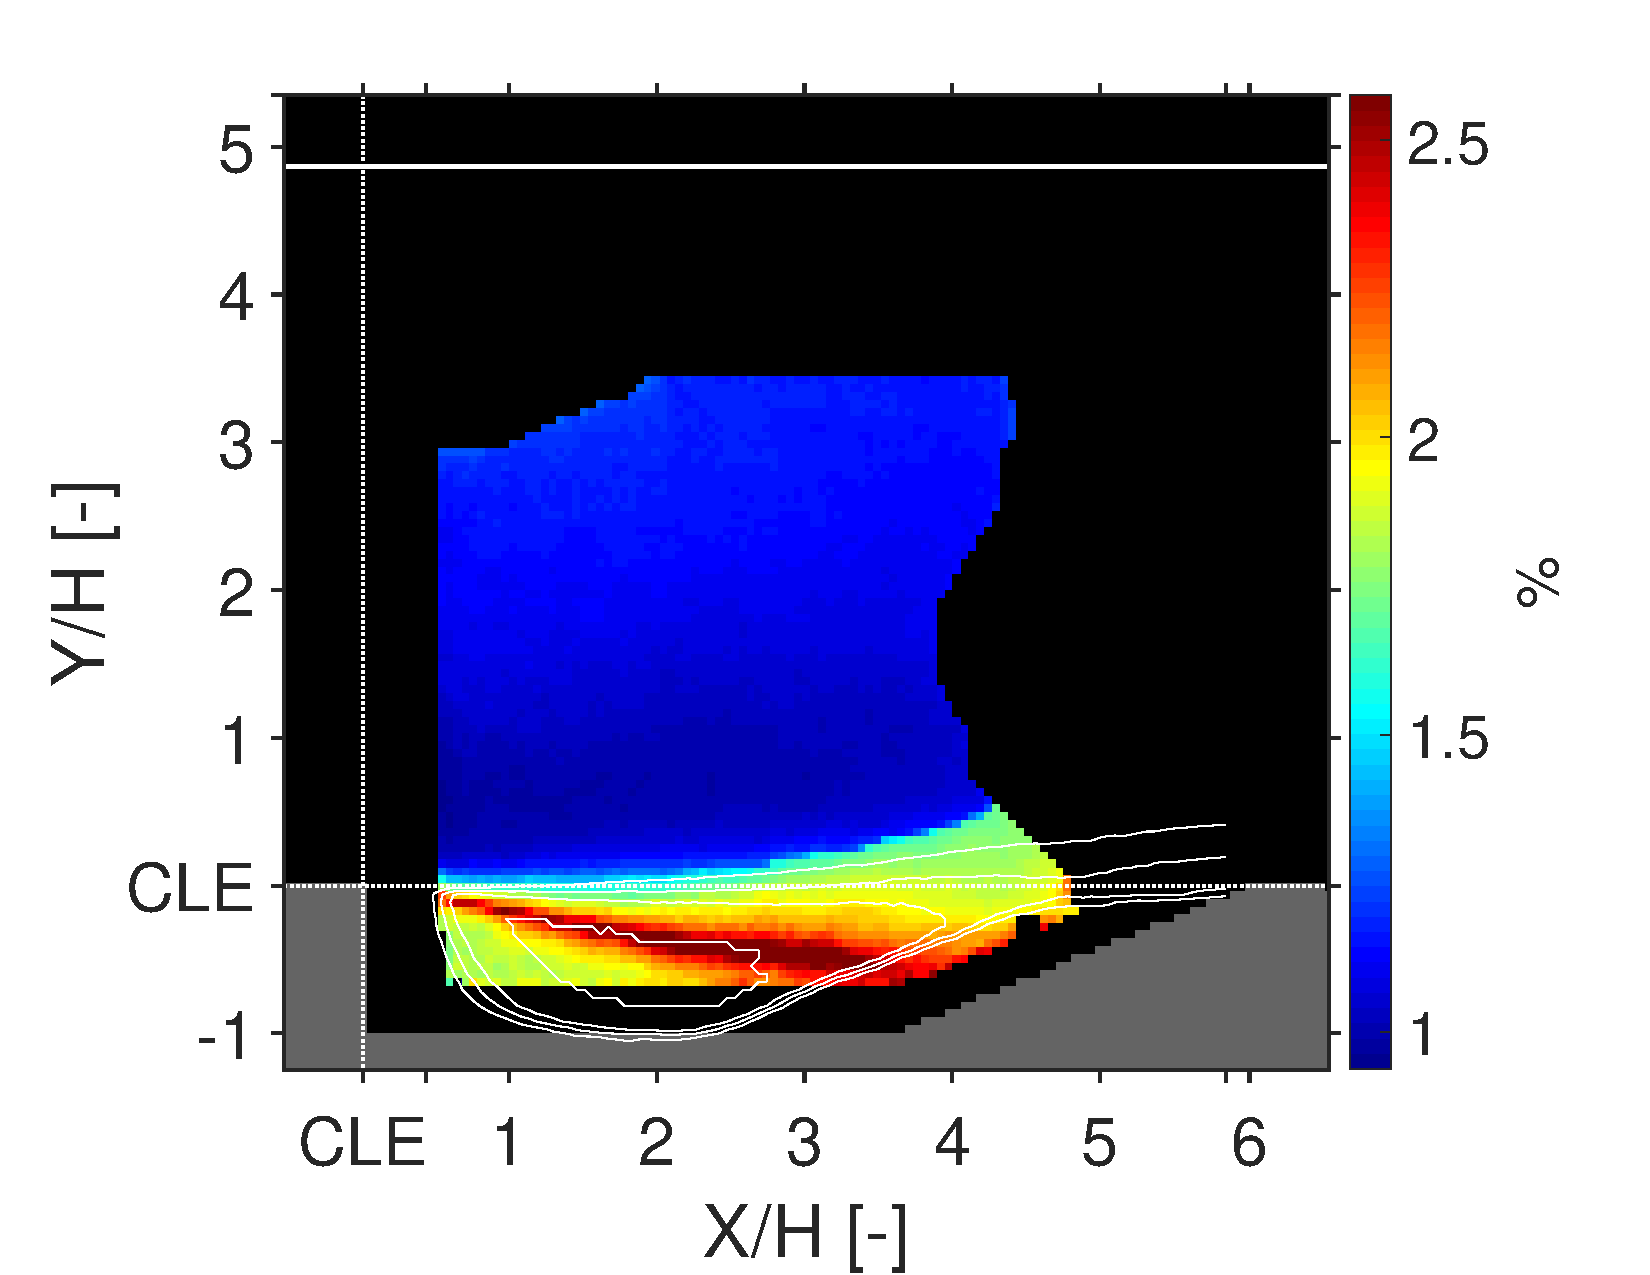
\includegraphics[width=3in, trim=0.3in 0in 0.1in 0.1in, clip]{figures/B1/whole_statistics/B1_TI}}
        \hspace{0.2in}
\subcaptionbox{Turbulent kinetic energy.\label{fig:B1_Uy_TKE}}
{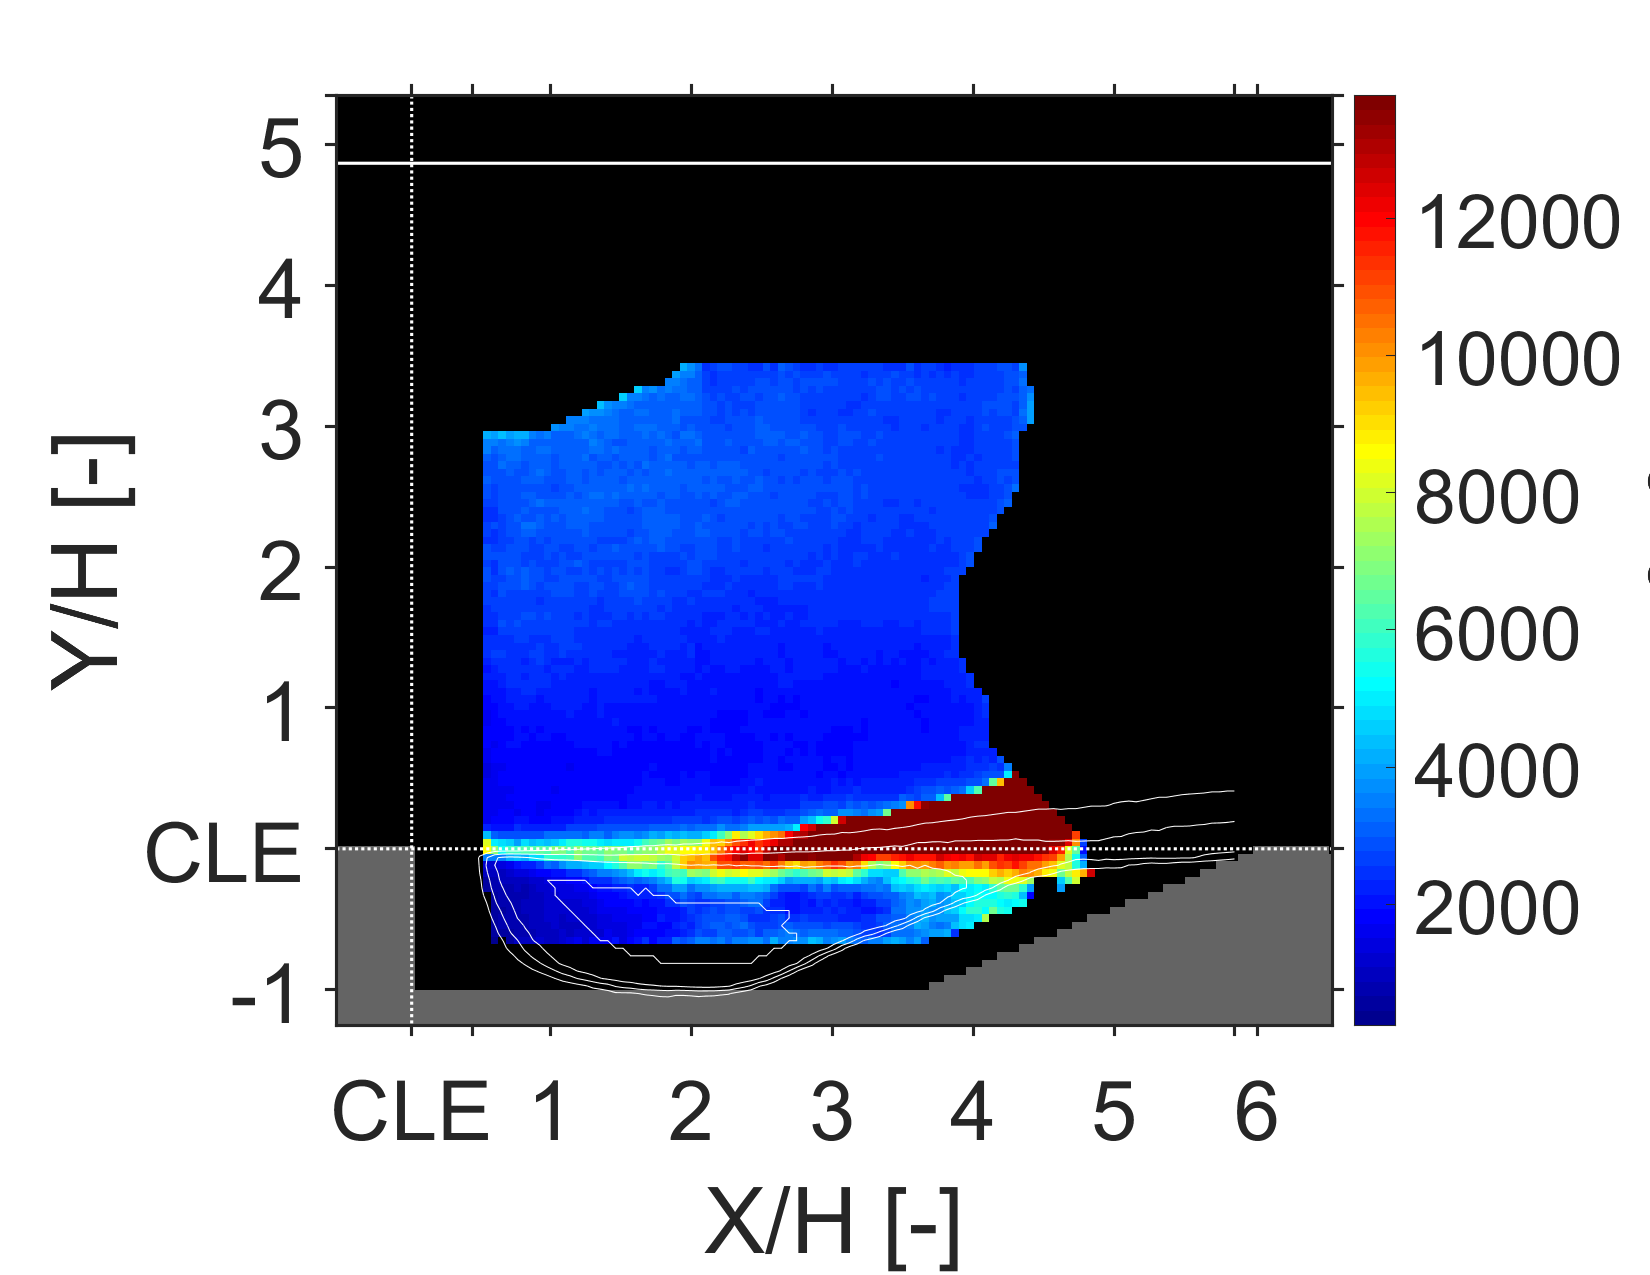
\includegraphics[width=3in,trim=0 0 1.3cm 0, clip]{figures/B1/whole_statistics/B1_TKE}
\rotatebox{90}{\hspace{1.15in}\footnotesize$\mathrm{[m^2/s^2]}$}}
\caption{Fluctuation energy indicators with flame intermittency contours}\label{fig:ch3_UxTKETI_PIVPLIF}
\end{figure}

\subsection*{Conditional velocities}\label{sec:ch3_cond_vel}
Figure \ref{fig:B2_all_cond_AVG} shows the mean absolute and relative conditional velocities with overlayed flame intermittency contours in white. The reactants and products axial velocity values and trends are similar to each other (see Figs. \ref{fig:B1_Ux_AVG_reactants} and \ref{fig:B1_Ux_AVG_products}), while the reactant transverse velocities below the cavity-freestream interface indicate reactants are entering the cavity and the product transverse velocities above the cavity-freestream interface indicate that products are escaping the cavity (see Figs. \ref{fig:B1_Uy_AVG_reactants} and \ref{fig:B1_Ux_AVG_products}). Transverse velocities are negative for both the products and reactants in the shear layer (Figs. \ref{fig:B1_Uy_AVG_reactants} and \ref{fig:B1_Uy_AVG_products}), but these velocities may change sign towards the aft end of the ramp where measurements were not possible. The difference between the reactant and the product mean velocities (Figs. \ref{fig:B1_relative_Ux_AVG_conditional} and \ref{fig:B1_relative_Uy_AVG_conditional}) indicates an upwards and backwards flow of the products relative to the reactants with mean velocity on the order of 1-10 m/s, in which reactants flow into products regions to ignite, transform into products, and flow out against incoming premixed flow.

Analysis of mass flux can reveal whether mass is accumulated and subsequently ejected at the cavity-freestream boundary. Because the measurement is two-dimensional, no spanwise flow can be taken into account.  The mass flux calculation also requires knowledge of the density, unavailable from the present measurements. Nonetheless, the direction of mass transfer may be inferred from the average transverse velocity at the cavity interface at $y/H=0$, shown in Fig. \ref{fig:ch3_cavity_interface_flux}. 
Both the products and reactants are on average flowing into the cavity with the exception of the region closest to the CLE, where velocities are zero. The hidden region past $x/H=5$ is expected to follow the increasing trend seen between $x/H=$ 4 to 5 in Fig. \ref{fig:ch3_cavity_interface_flux} such that the mean transverse flux along the entire cavity interface equals zero and mass is conserved. Therefore, mass transfer out of the cavity mostly occurs near the ramp. This observation, in conjunction with the 60$\%$ flame intermittency at the downstream end of the cavity interface (see Fig. \ref{fig:B1_PLIF}), hints at ejection events that compensate for the mass and heat accumulated in the cavity over the remaining 40$\%$ of the time. Ensemble statistics do not allow further investigation into the disrupting ejection events suggested by the above results. In the following section, the problem is further studied using instantaneous measurements.

\begin{figure}
\centering
        \subcaptionbox{Reactants $\bar{U}_{x,R}$\label{fig:B1_Ux_AVG_reactants}}
        {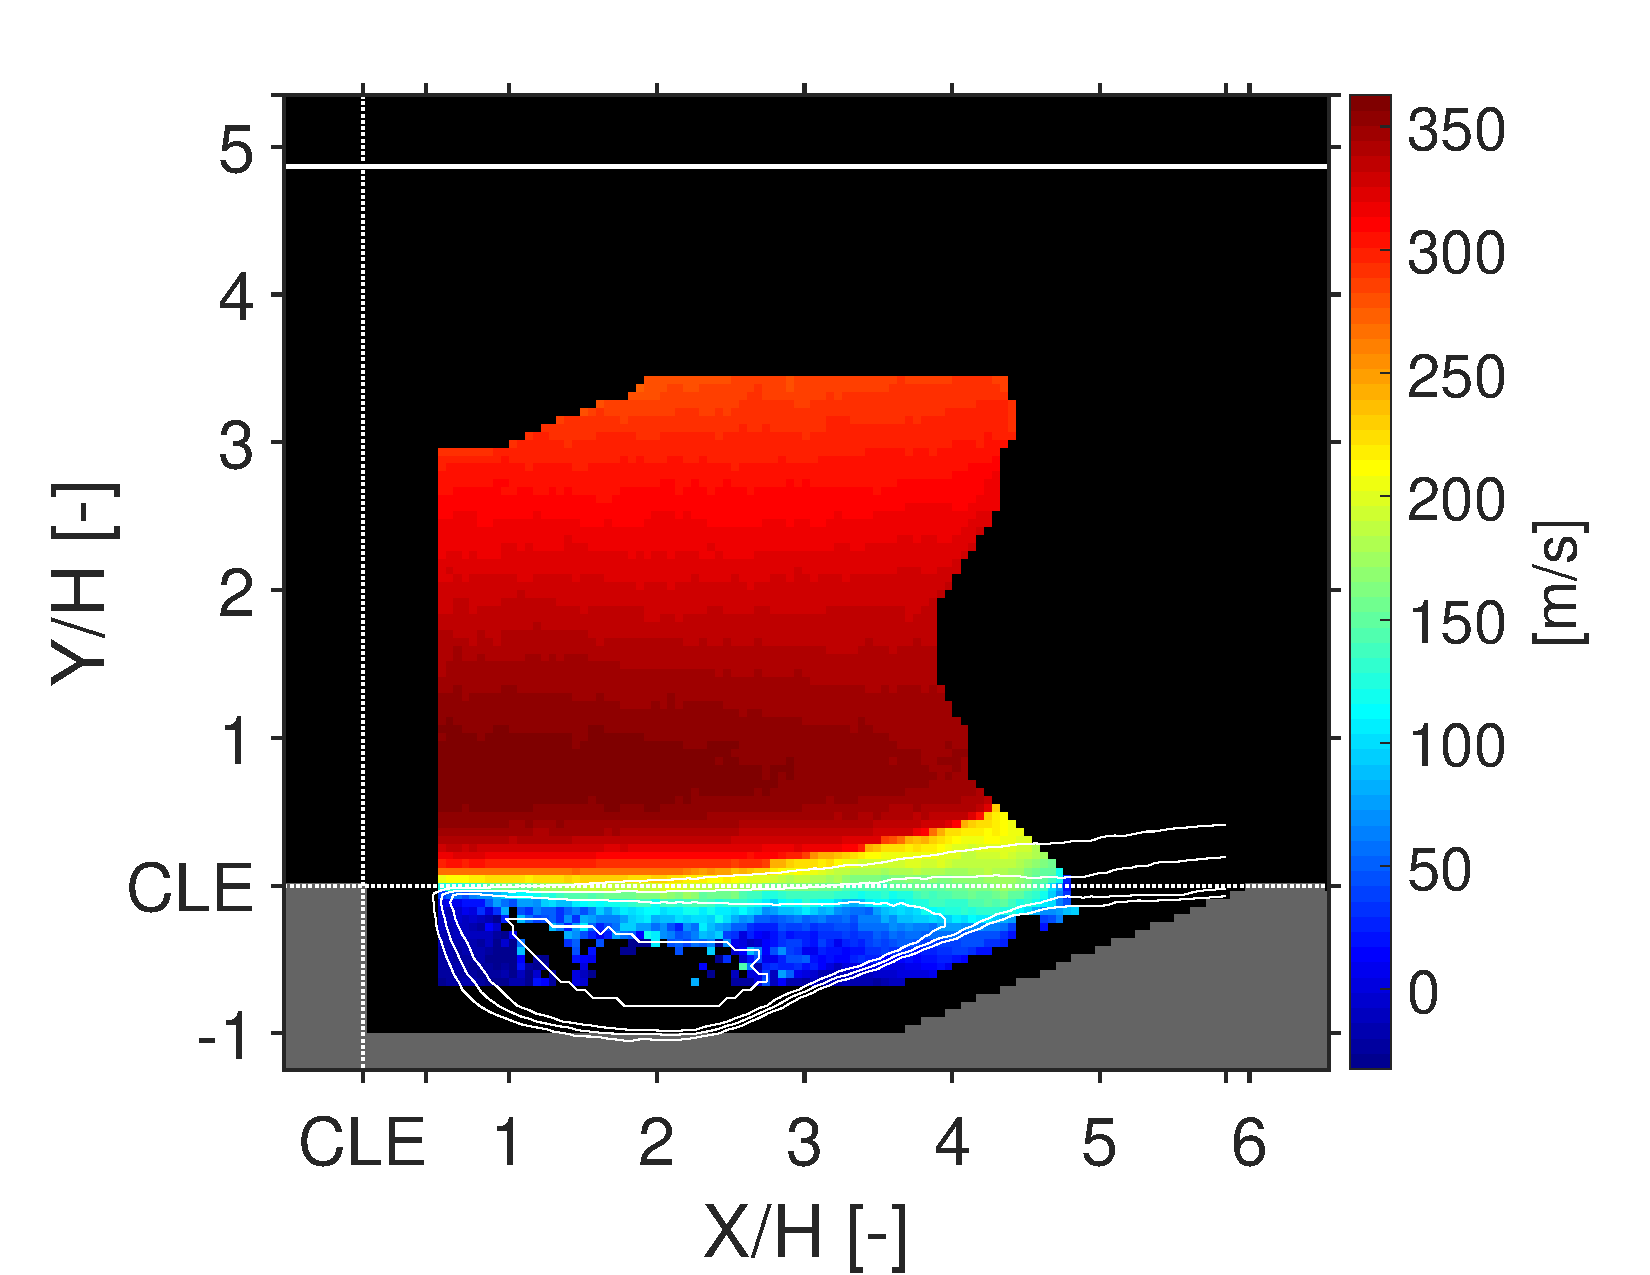
\includegraphics[width=3in,trim=0.35in 0 0.42in 0, clip]{figures/B1/cond_statistics/B1_Ux_AVG_reactants}} \hspace{0.4cm}
        \subcaptionbox{Products $\bar{U}_{x,P}$\label{fig:B1_Ux_AVG_products}}
        {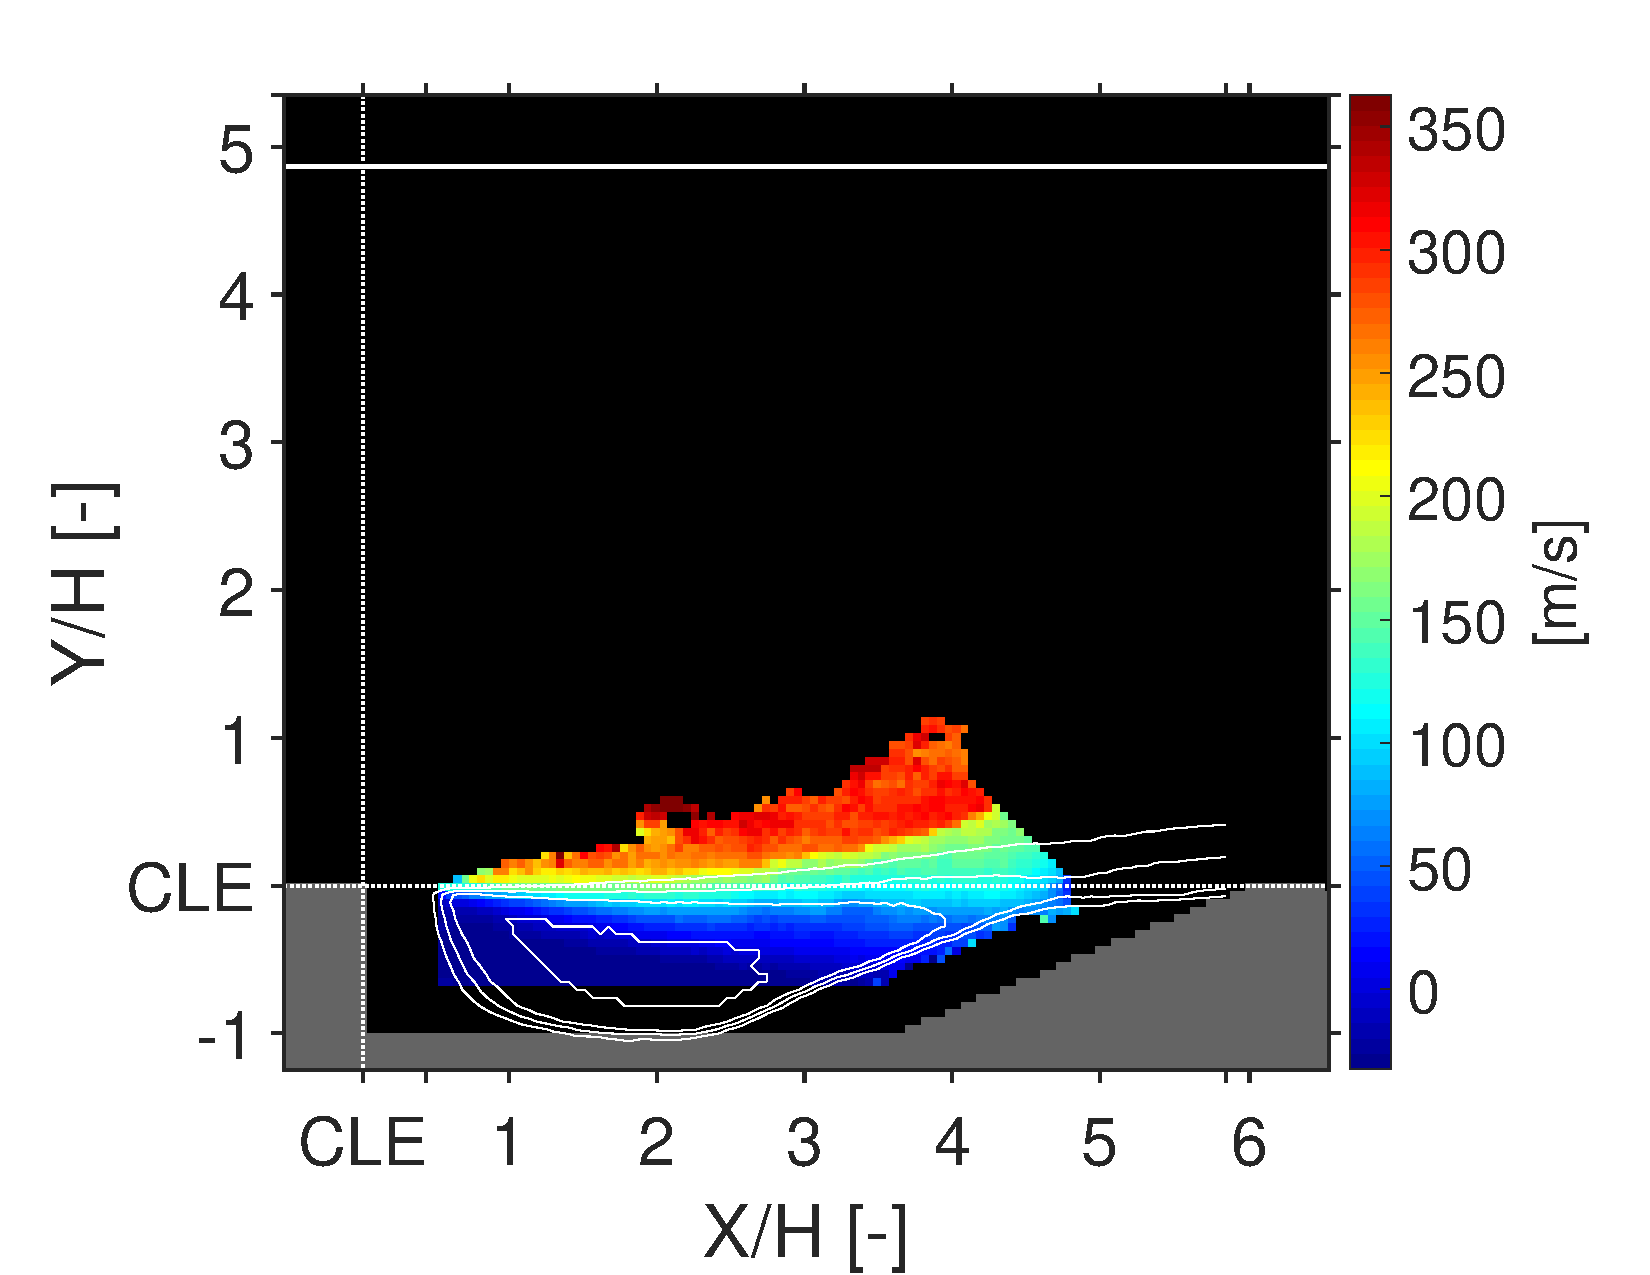
\includegraphics[width=3in,trim=0.35in 0 0.42in 0, clip]{figures/B1/cond_statistics/B1_Ux_AVG_products}}
        \newline
        
        \subcaptionbox{Reactants $\bar{U}_{y,R}$\label{fig:B1_Uy_AVG_reactants}}
        {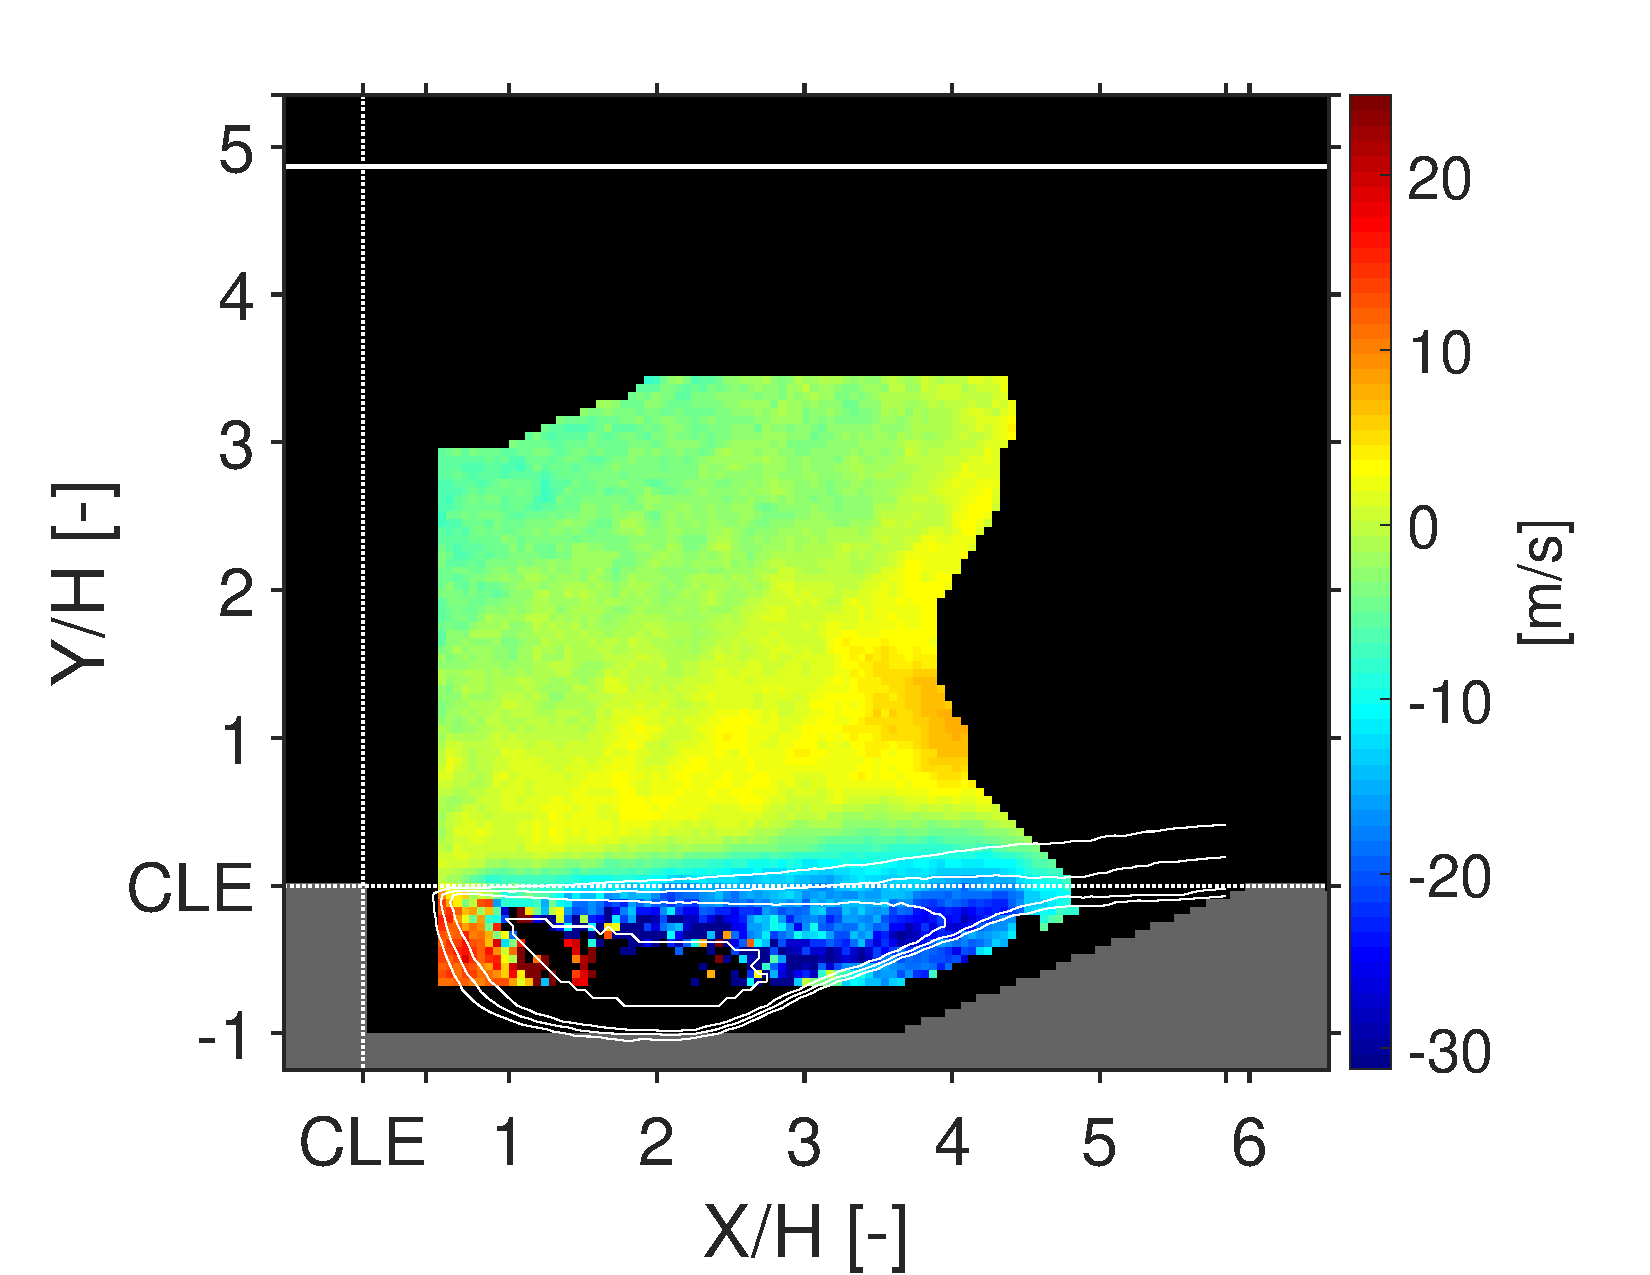
\includegraphics[width=3in,trim=0.35in 0 0.42in 0, clip]{figures/B1/cond_statistics/B1_Uy_AVG_reactants}} \hspace{0.4cm}
        \subcaptionbox{Products $\bar{U}_{y,P}$\label{fig:B1_Uy_AVG_products}}
        {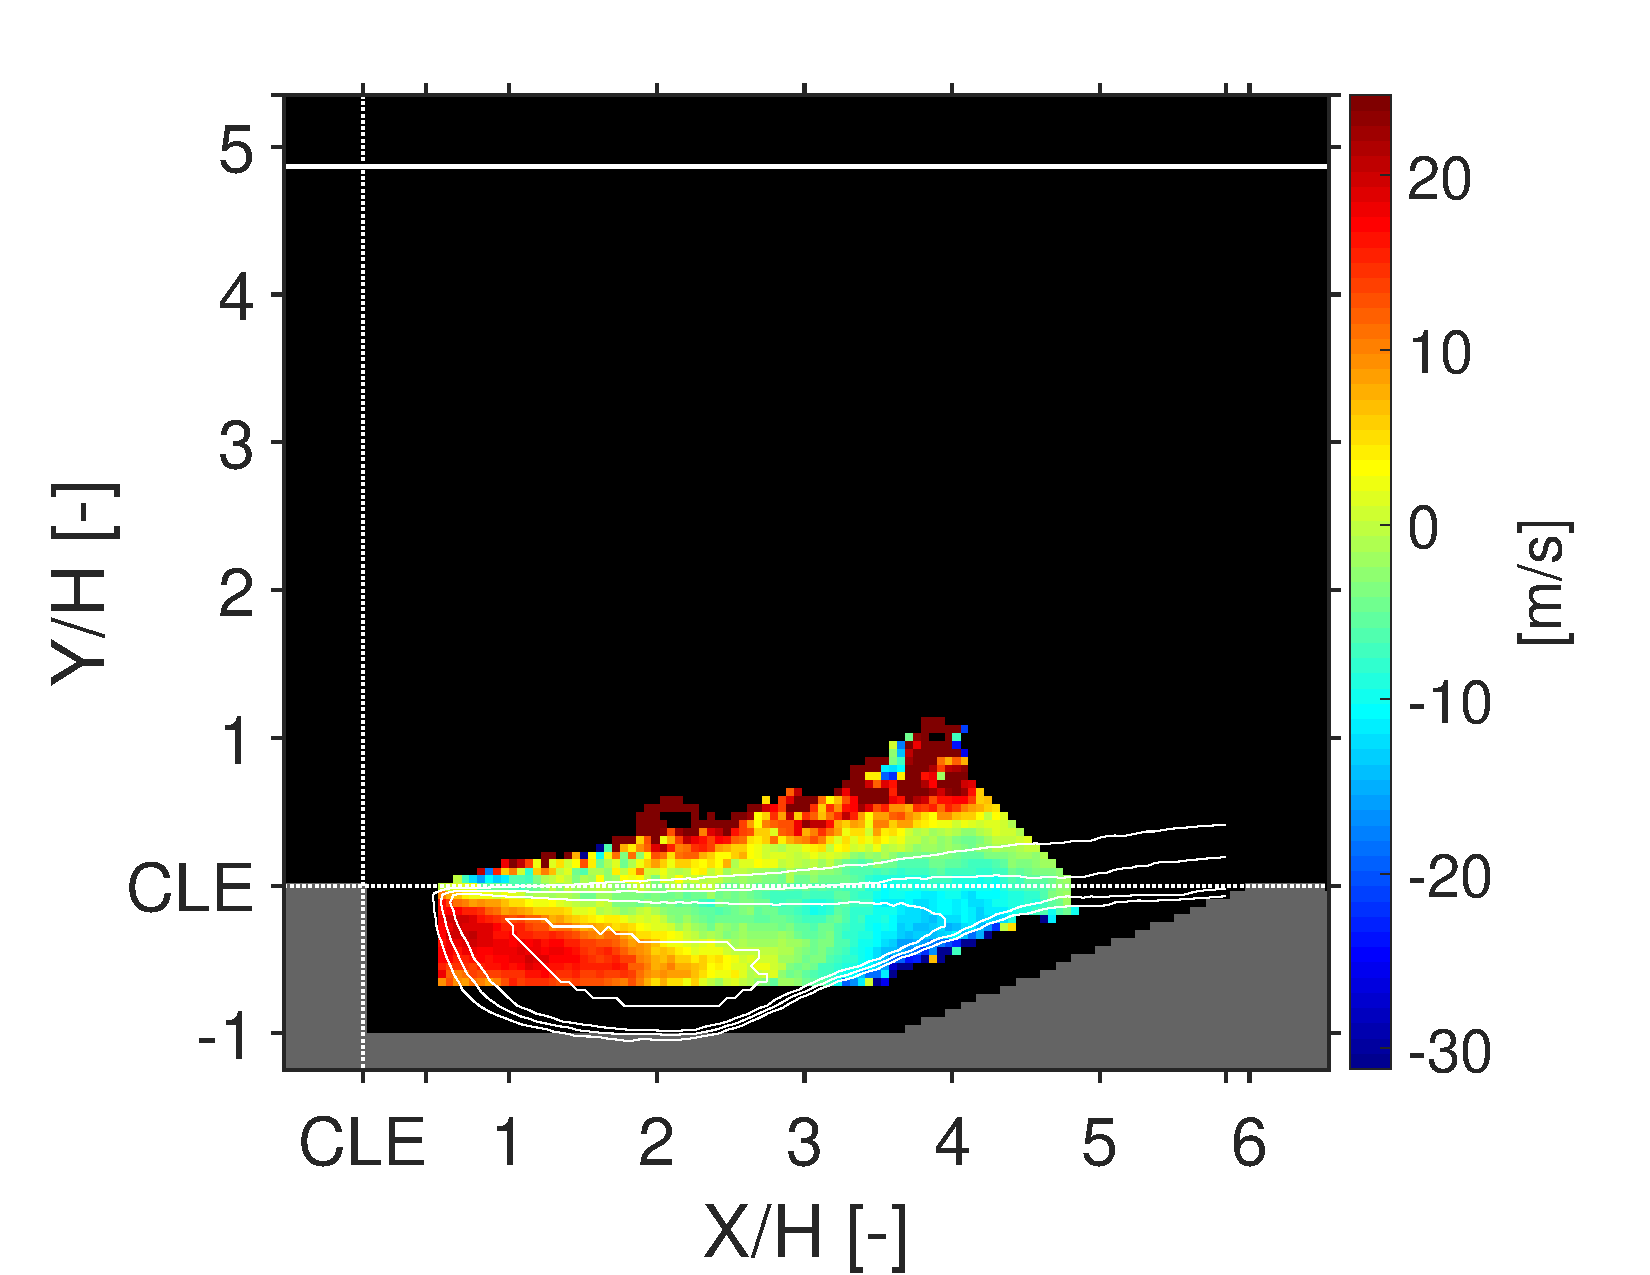
\includegraphics[width=3in,trim=0.35in 0 0.42in 0, clip]{figures/B1/cond_statistics/B1_Uy_AVG_products}}
        \newline
        
        \subcaptionbox{Axial velocities of products relative to reactants \\$\bar{U}_{x,P}-\bar{U}_{x, R}$\label{fig:B1_relative_Ux_AVG_conditional}}
        {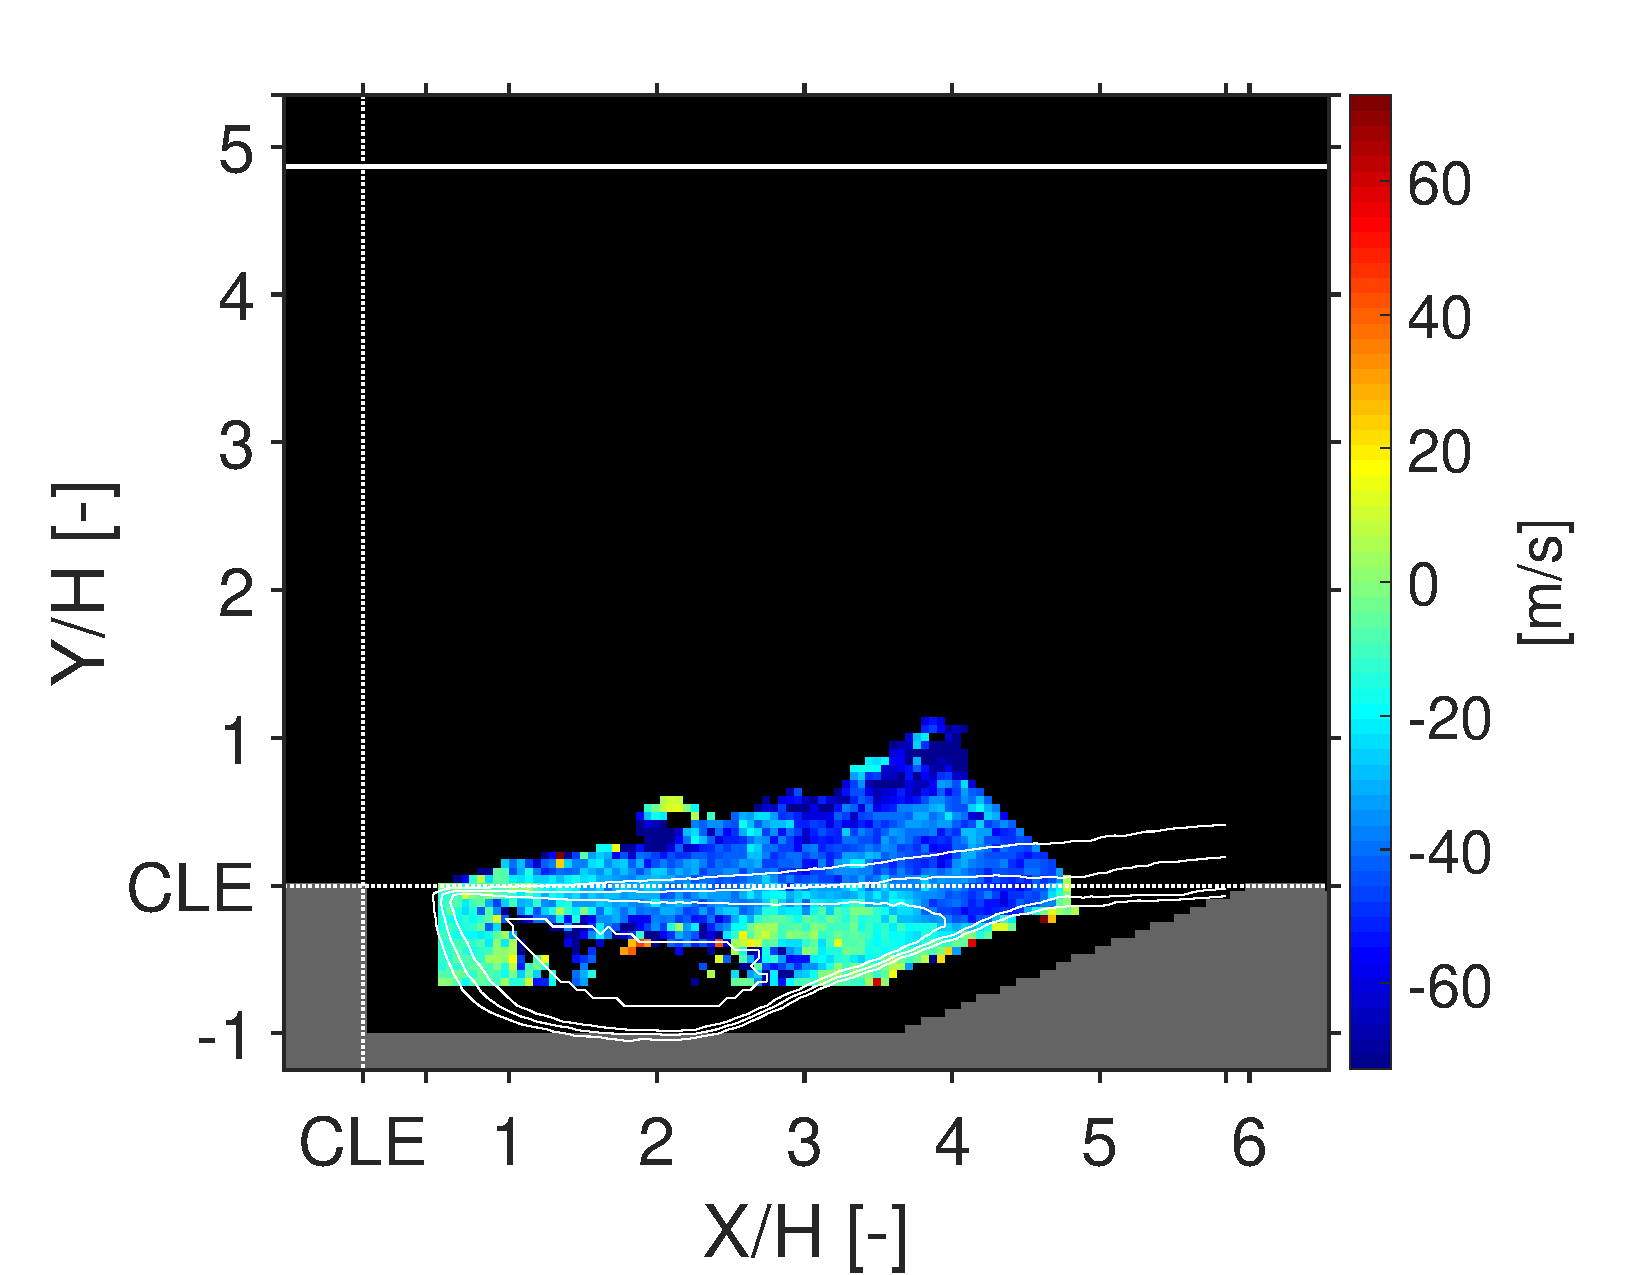
\includegraphics[width=3in,trim=0.35in 0 0.42in 0, clip]{figures/B1/cond_statistics/B1_relative_Ux_AVG_conditional}} \hspace{0.4cm}
        \subcaptionbox{Transverse velocities of products relative to reactants $\bar{U}_{y,P}-\bar{U}_{y, R}$\label{fig:B1_relative_Uy_AVG_conditional}}
        {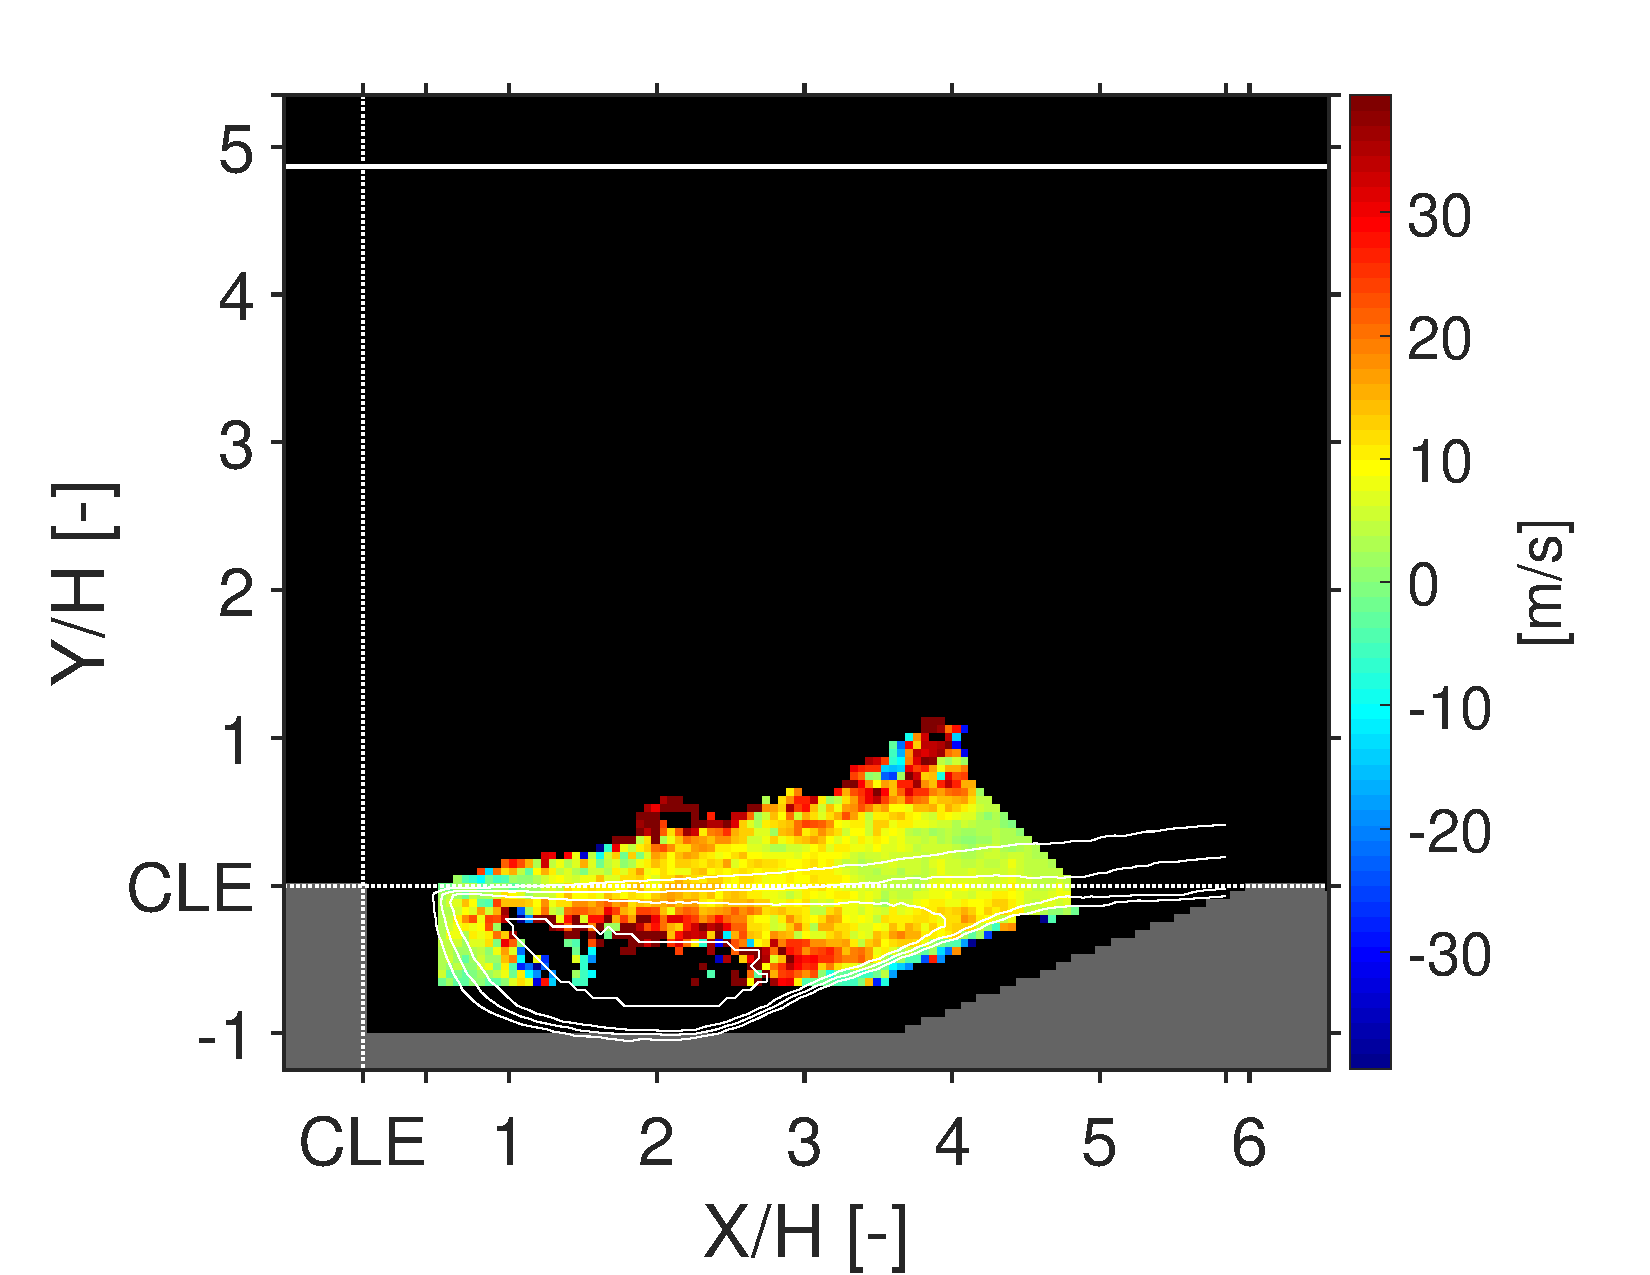
\includegraphics[width=3in,trim=0.35in 0 0.42in 0, clip]{figures/B1/cond_statistics/B1_relative_Uy_AVG_conditional}}
\caption{Mean conditional velocity fields with flame intermittency contours}\label{fig:B2_all_cond_AVG}
\end{figure}

\begin{figure}
\centering
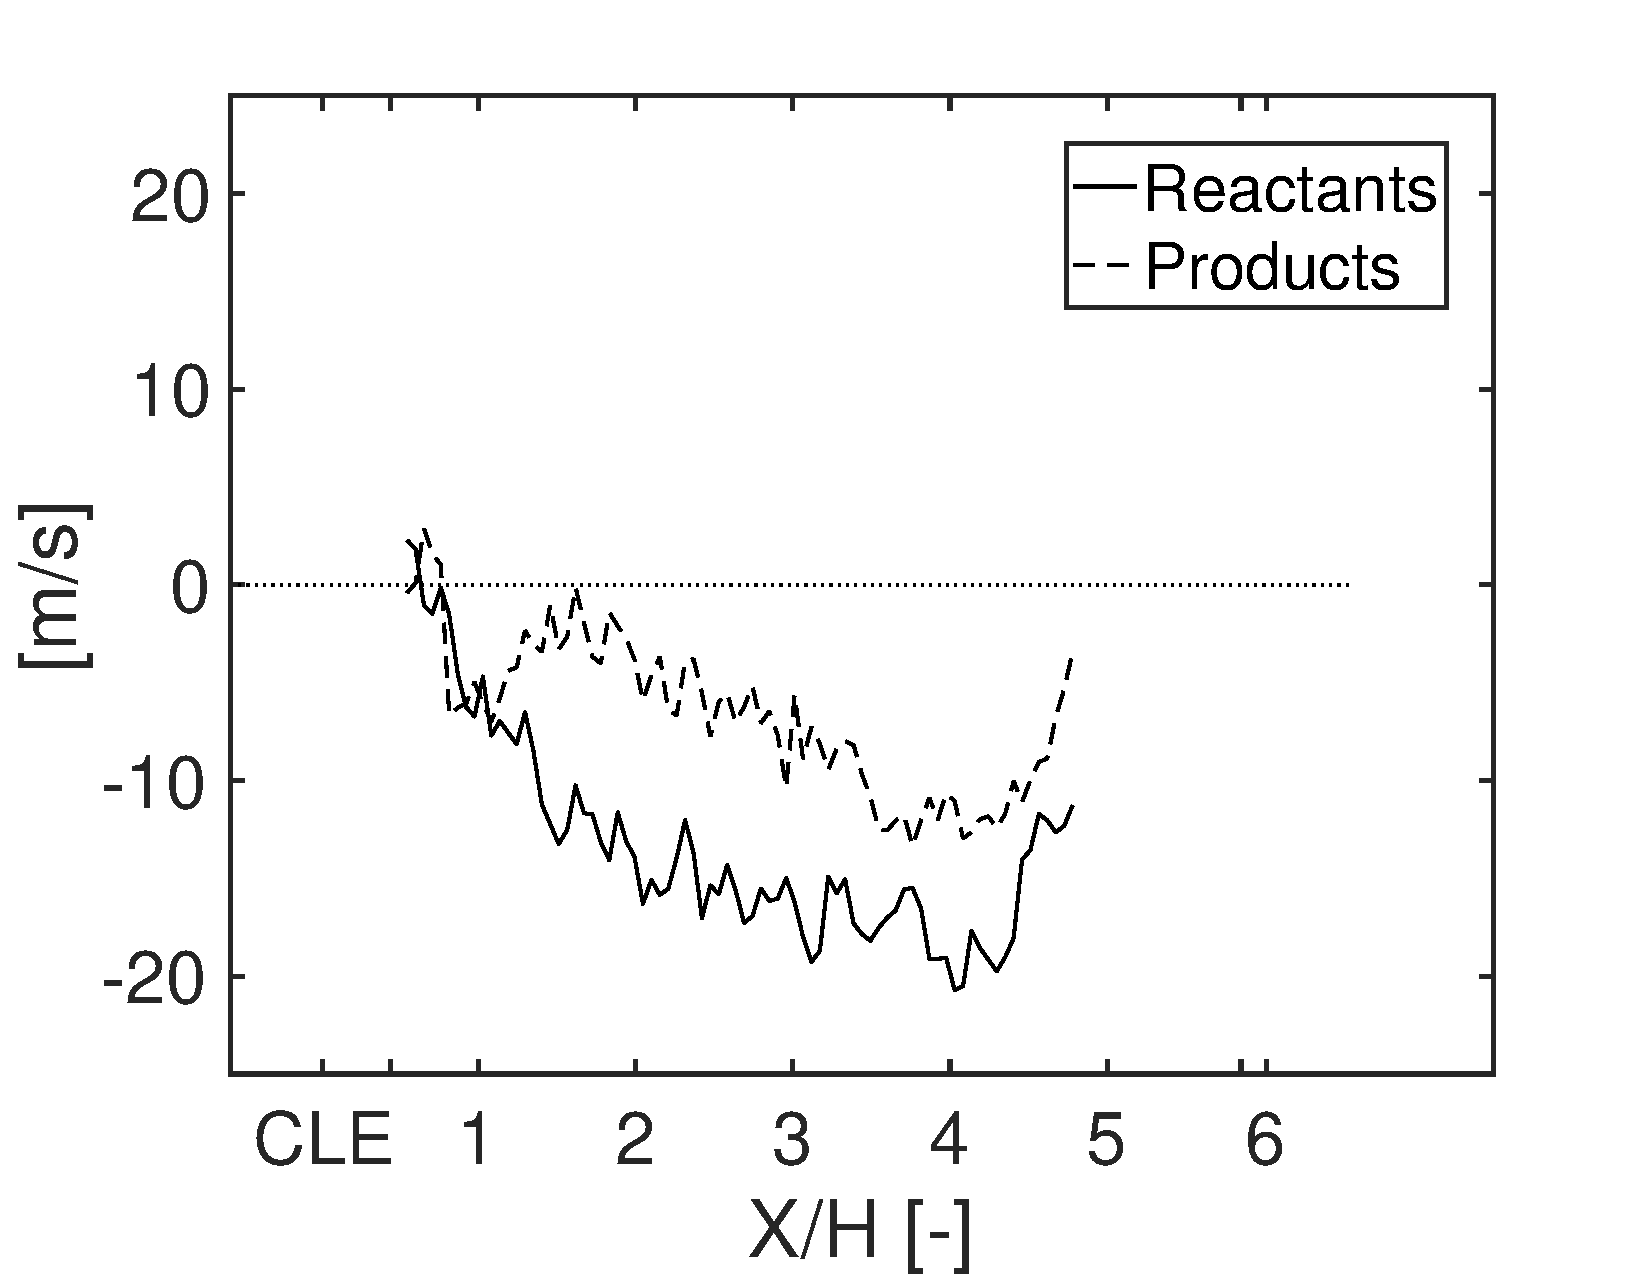
\includegraphics[width=3.25in]{figures/B1/flux/B1_average_YH0_flux} 
\caption{Mean transverse velocities at the cavity interface at $y/H=0$ \label{fig:ch3_cavity_interface_flux}}
\end{figure}


\section*{Combustion dynamics}\label{sec:ch3_cavity_dynamics}
The combined PIV and PLIF fields may be used as complementary inputs to gain insights into the unsteady flame structure. Randomly-sampled images of the OH structures are observed throughout the dataset, which may be sorted into three main categories of state. In state 1, the flame is contained within the cavity before the ramp ($y/H<0$ and $x/H<4$). In state 2, the flame continuously extends past the cavity interface and ramp. In state 3, the extended flame is discontinuous.

The three states are consistent with the previously-stated hypothesis that thermoacoustic oscillations, due to coupling between the inlet shock-train and thermal throat, couple with combustion in the cavity \citep{WangWangSun2014, TuttleCarterHsu2014, Kirik2017, AllisonFredericksonKirikEtAl2017}.  Thermoacoustic oscillation is associated with length scales on the order of the distance between the shock train and the thermal throat. Thermoacoustic oscillation frequencies are much smaller than the frequencies of the largest cavity shear layer eddies, the freestream turbulence, and the acoustic oscillations of the cavity. Therefore, these states are not consistent with normal cavity oscillations.   The combustion cycle suggested below consists of periodic combustion product ejection through shear layer detachment from the cavity ramp. 

The present PIV-PLIF acquisition frequency of 10 Hz does not permit motions on the order of 100-1000 Hz to be resolved. However, a cyclical process may be proposed based on the identification of categories described above. Given that the combustion oscillation frequency is unlikely to be a harmonic of the PIV-PLIF acquisition frequency, one may assume that the combustion cycle is randomly captured over the available 2,000 measurements. With the additional input of the flow direction, physical inference, and the previous investigations on cavity flows listed in the introduction, the categories of instantaneous measurements may be sorted into a sequence of hypothetical states: 1-2-3.  Other orders are physically implausible. The state series 2-1-3 would imply that the extended part of the flame extinguishes before a separated flame self-ignites in the main duct flow. The state series 3-2-1 would have the separated flame self-ignite in the duct flow and propagate against the high-speed flow to connect with the upstream cavity flame.  Instantaneous measurements that illustrate these states are selected; Figs. \ref{fig:ch3_inst_B1} and \ref{fig:ch3_inst_B1vec} display velocity maps and streamlines, respectively, overlayed with an outline of the products region, as identified from PLIF. These figures also display measurements that appear to show transitions between states; these are labeled 2' (between states 2 and 3) and 3' (between states 3 and 1).  The streamlines of Fig. \ref{fig:ch3_inst_B1vec} shows that eddies are present that vary in size and location across the various states.  Figure \ref{fig:ch3_inst_ST} displays the swirling strength of vortices, which allows better localization of the strongest eddies independently of the reference frame  \citep{Adrian2000}. 

\begin{figure}
\centering
\subcaptionbox{State 1\label{fig:B1_Frame1}}
                {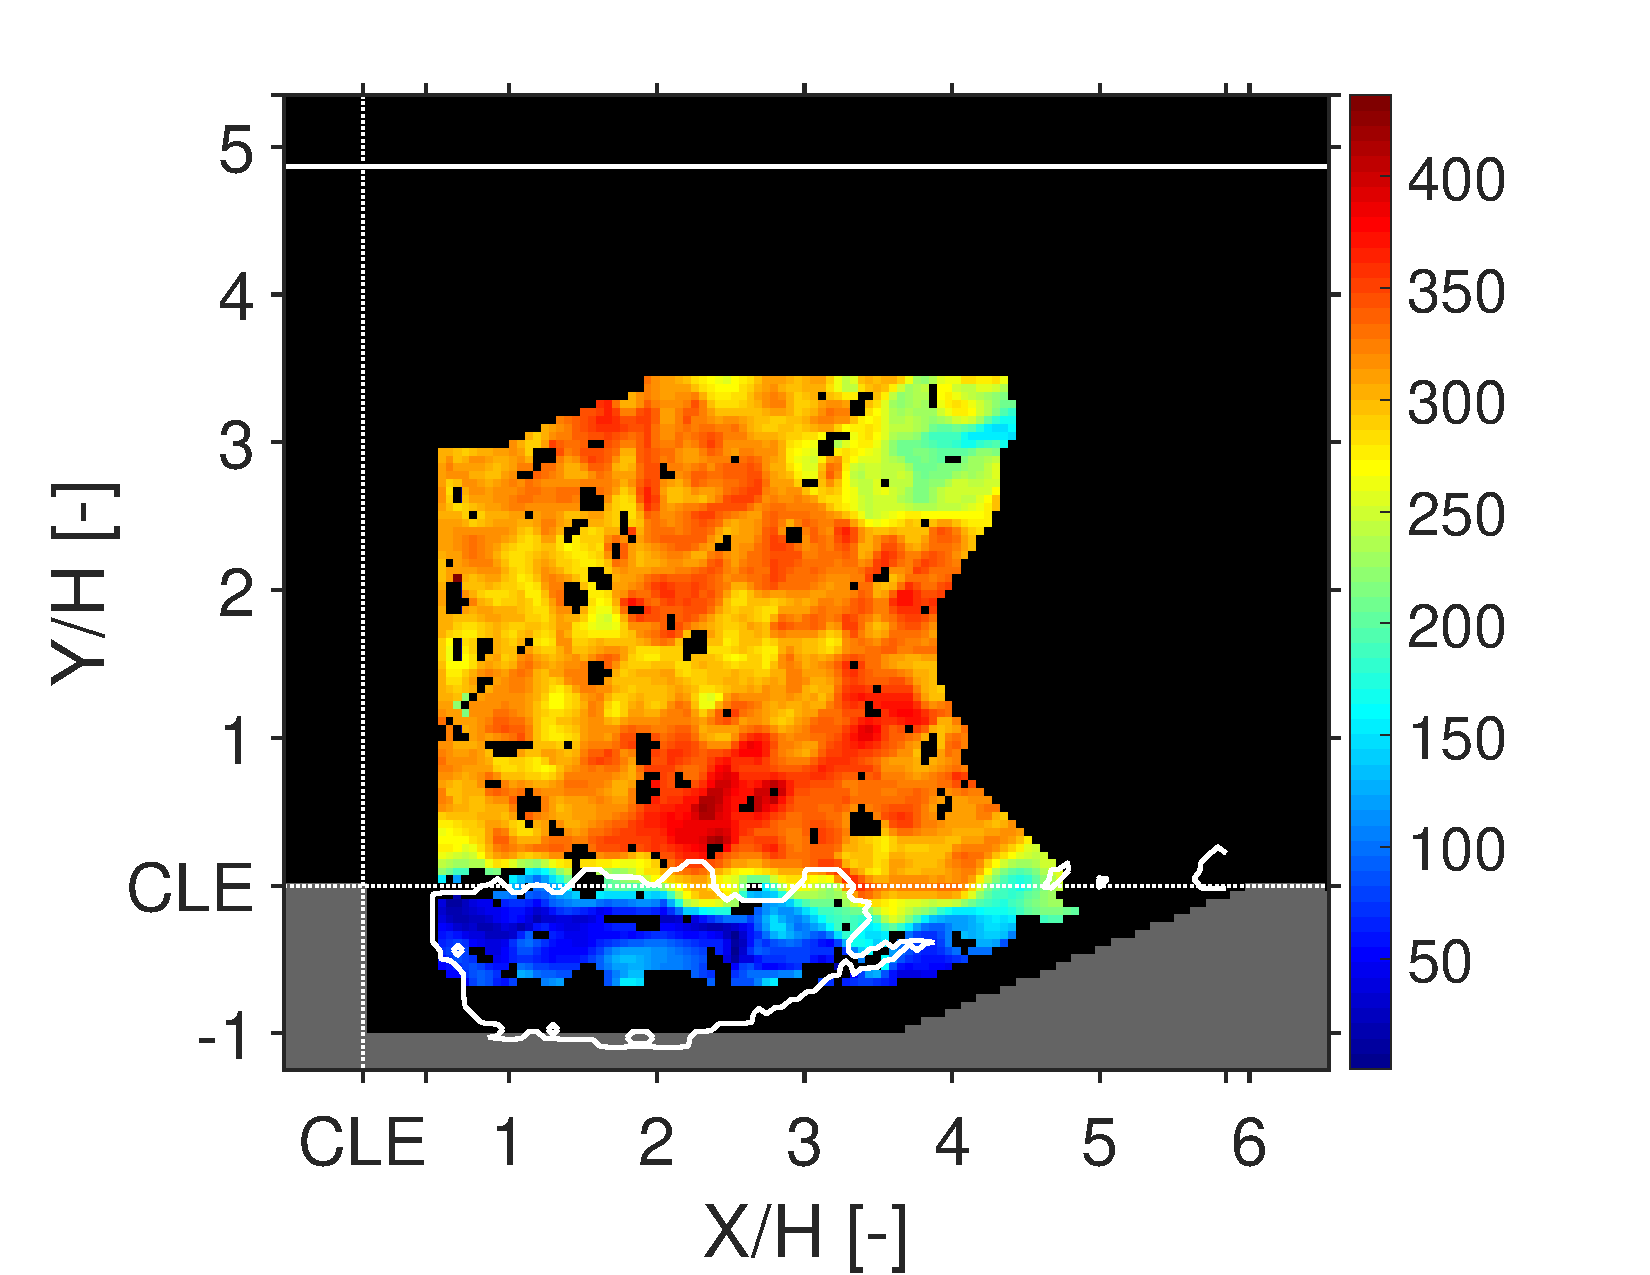
\includegraphics[width=3in,trim=0.35in 0 0.65in 0, clip]{figures/B1/combustion_instability/1/absolute_vel/B1_Frame331.pdf}\rotatebox{90}{\hspace{1.3in}\footnotesize$\mathrm{[m/s]}$}}
                \hspace{0.4cm}
\subcaptionbox{State 2\label{fig:B1_Frame2}}
                {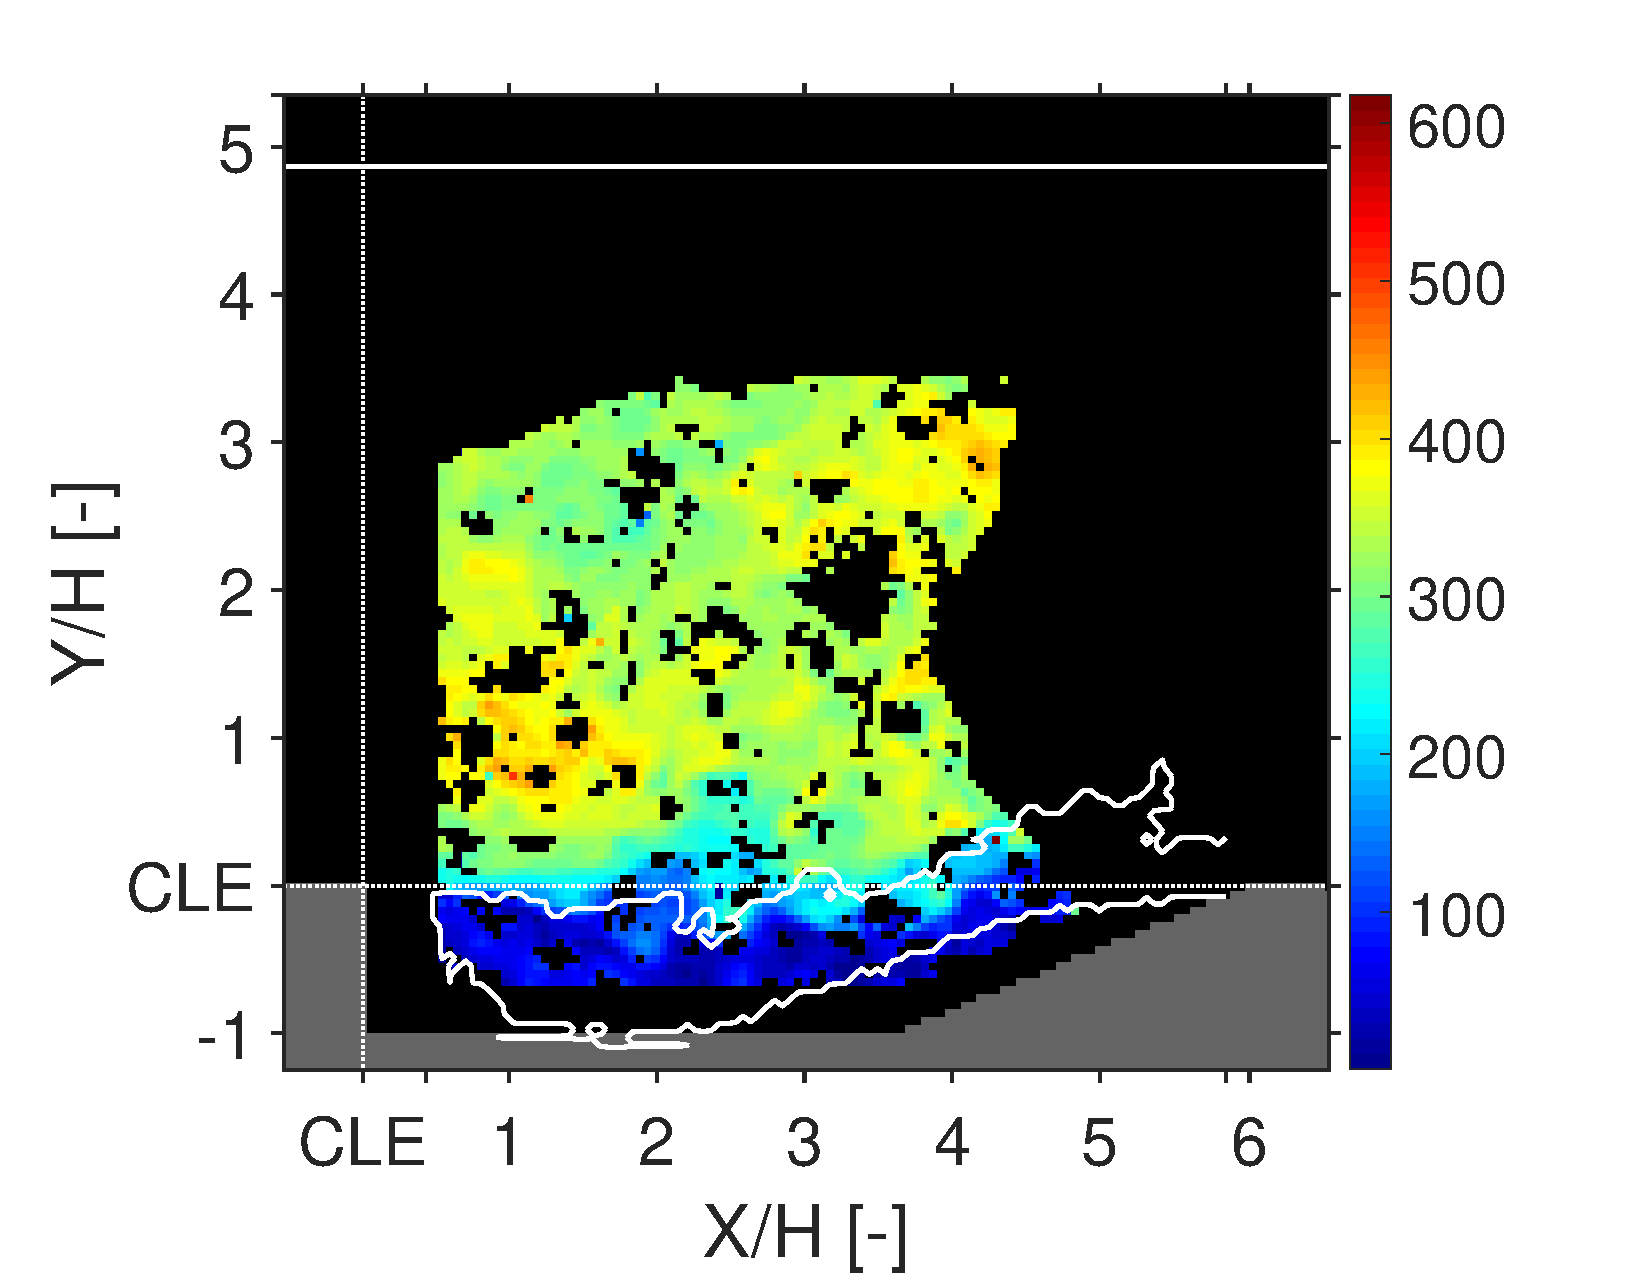
\includegraphics[width=3in,trim=0.35in 0 0.65in 0, clip]{figures/B1/combustion_instability/2/absolute_vel/B1_Frame329.pdf}\rotatebox{90}{\hspace{1.3in}\footnotesize$\mathrm{[m/s]}$}}
                \newline
\subcaptionbox{State 2'\label{fig:B1_Frame3}}
                {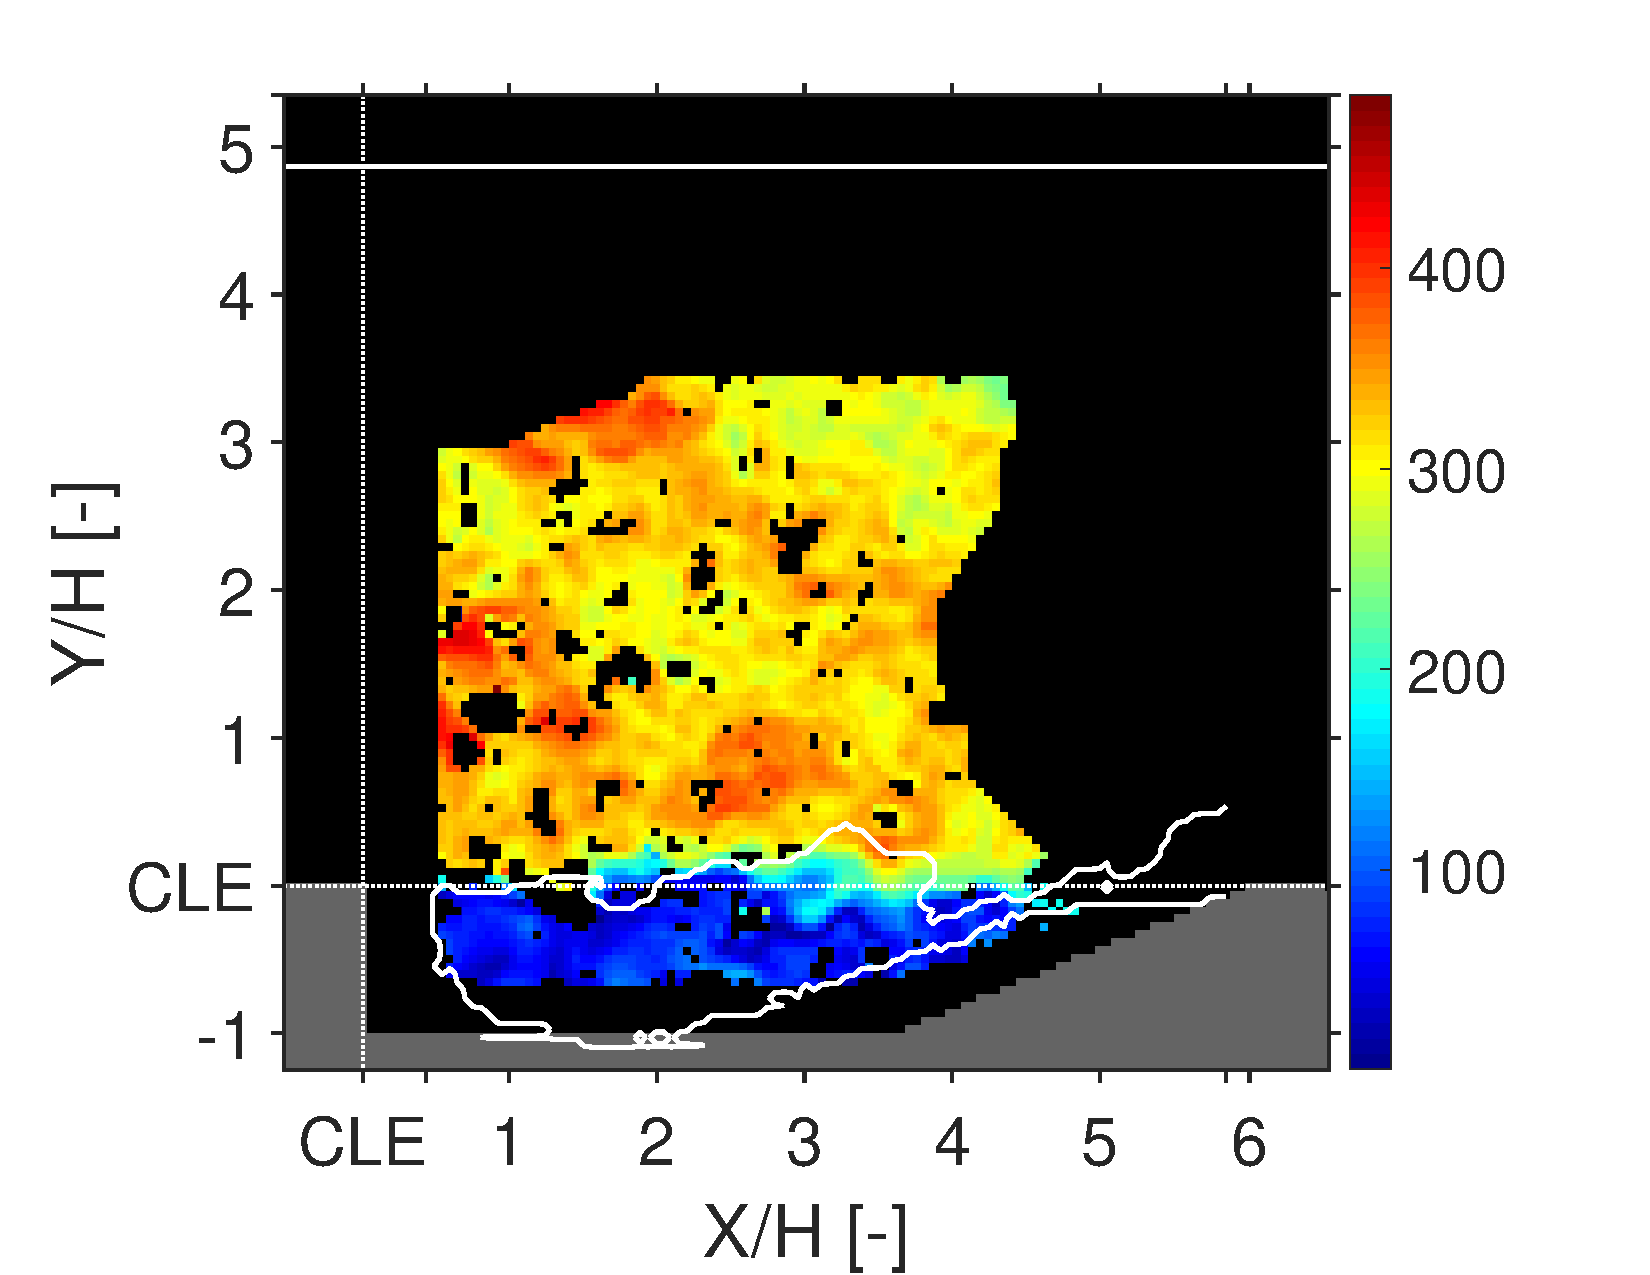
\includegraphics[width=3in,trim=0.35in 0 0.65in 0, clip]{figures/B1/combustion_instability/3/absolute_vel/B1_Frame342.pdf}\rotatebox{90}{\hspace{1.3in}\footnotesize$\mathrm{[m/s]}$}}
                \hspace{0.4cm}
\subcaptionbox{State 3\label{fig:B1_Frame4}}
                {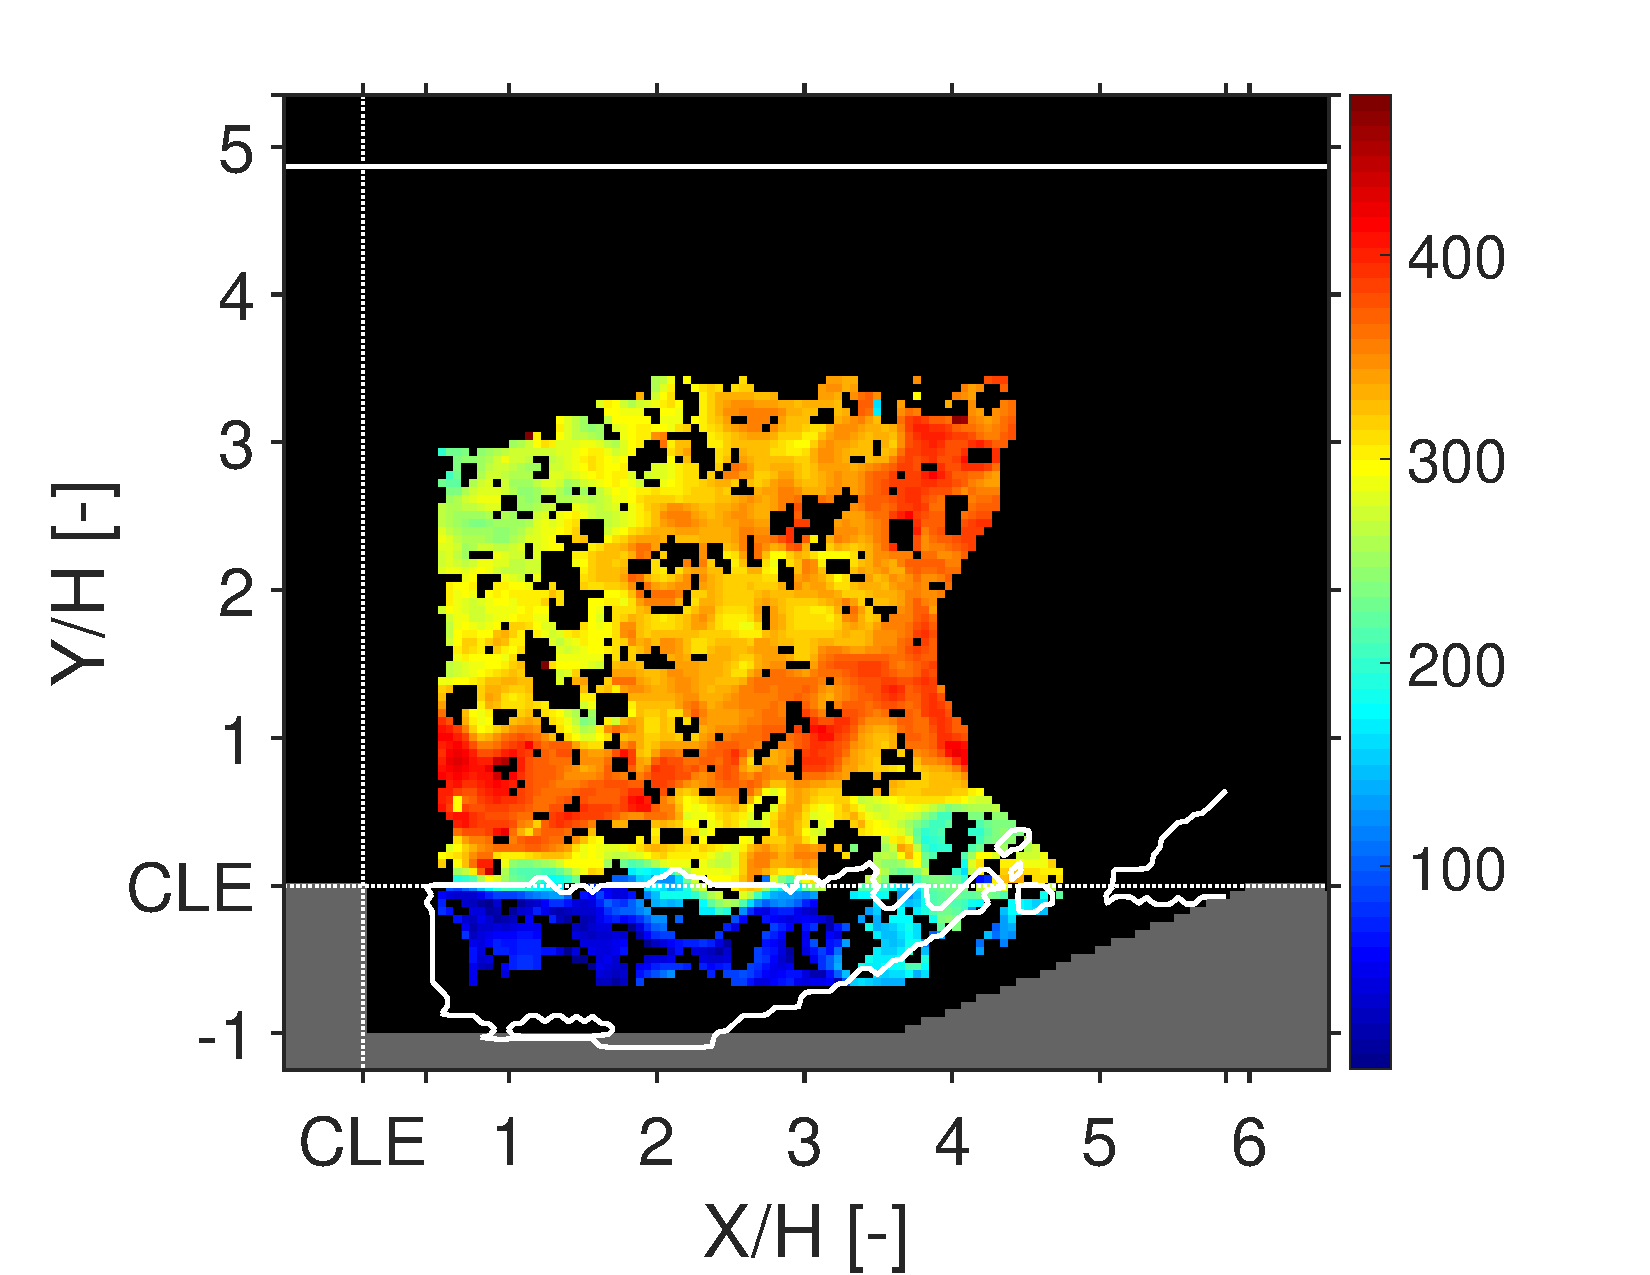
\includegraphics[width=3in,trim=0.35in 0 0.65in 0, clip]{figures/B1/combustion_instability/3/absolute_vel/B1_Frame339.pdf}\rotatebox{90}{\hspace{1.3in}\footnotesize$\mathrm{[m/s]}$}}
                \newline
 \subcaptionbox{State 3'\label{fig:B1_Frame5}}
                {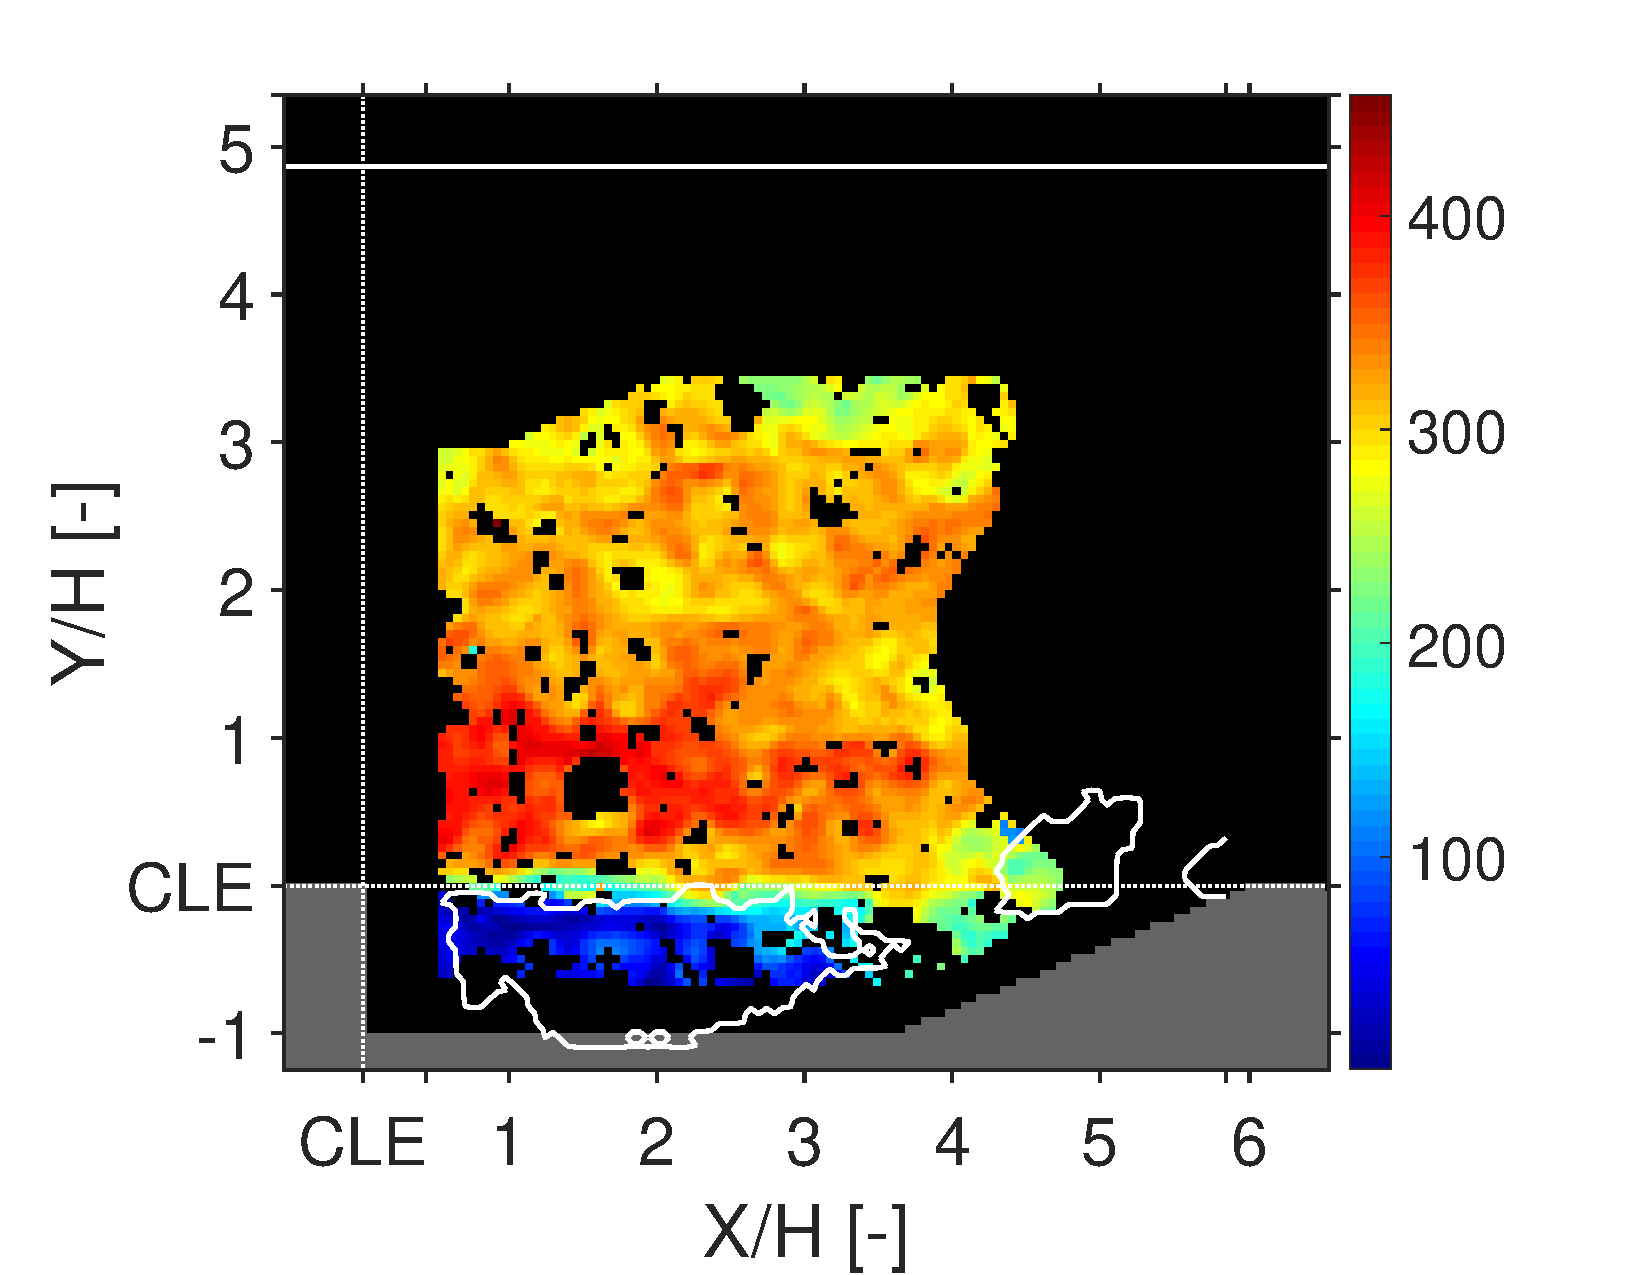
\includegraphics[width=3in,trim=0.35in 0 0.65in 0, clip]{figures/B1/combustion_instability/3/absolute_vel/B1_Frame306.pdf}\rotatebox{90}{\hspace{1.3in}\footnotesize$\mathrm{[m/s]}$}}
                \hspace{0.4cm}
        \subcaptionbox{State 2 with duct velocities below average\label{fig:B1_Frame6}}
                {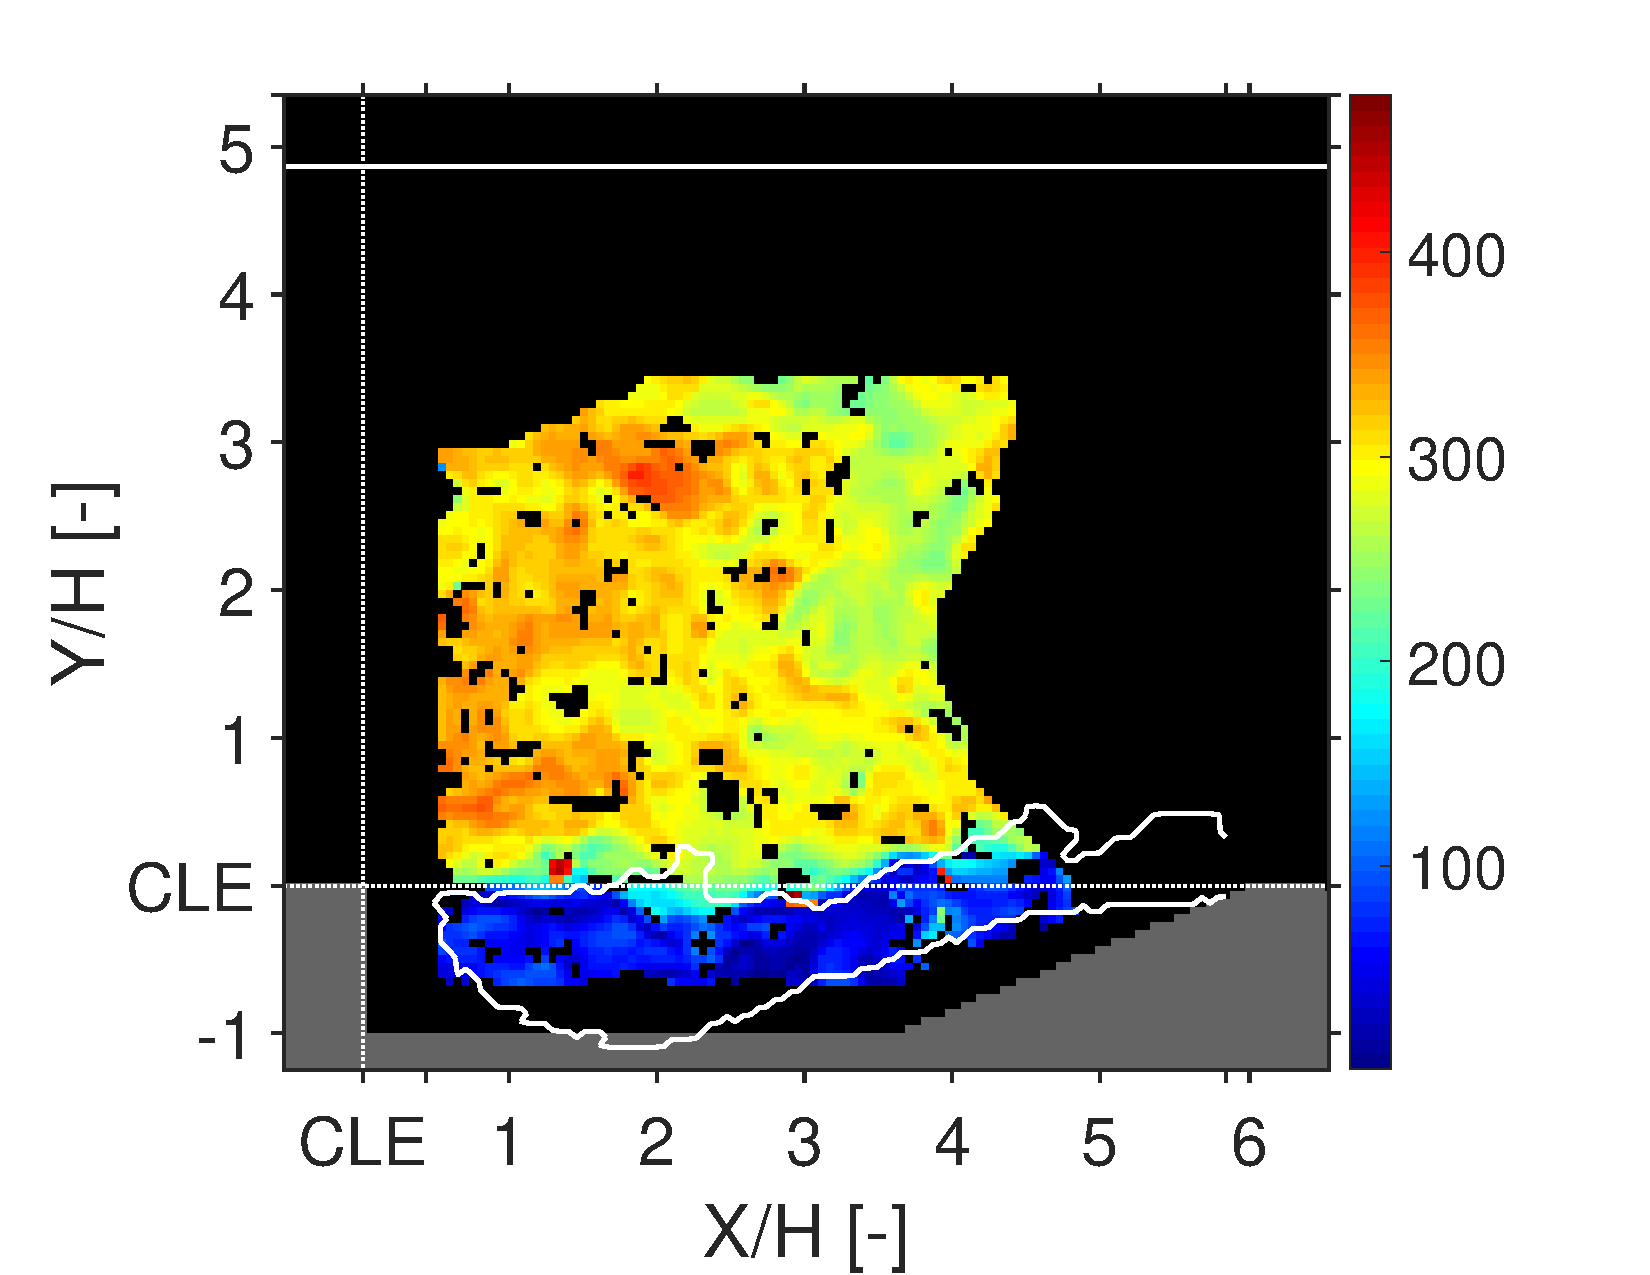
\includegraphics[width=3in,trim=0.35in 0 0.65in 0, clip]{figures/B1/combustion_instability/2/absolute_vel/B1_Frame301.pdf}\rotatebox{90}{\hspace{1.3in}\footnotesize$\mathrm{[m/s]}$}}
\caption{Velocity magnitude, select instantaneous PIV-PLIF frames.}\label{fig:ch3_inst_B1}
\end{figure}

% \begin{figure}
% \centering
% \subcaptionbox{State 1\label{fig:B1_Frame1}}
%         {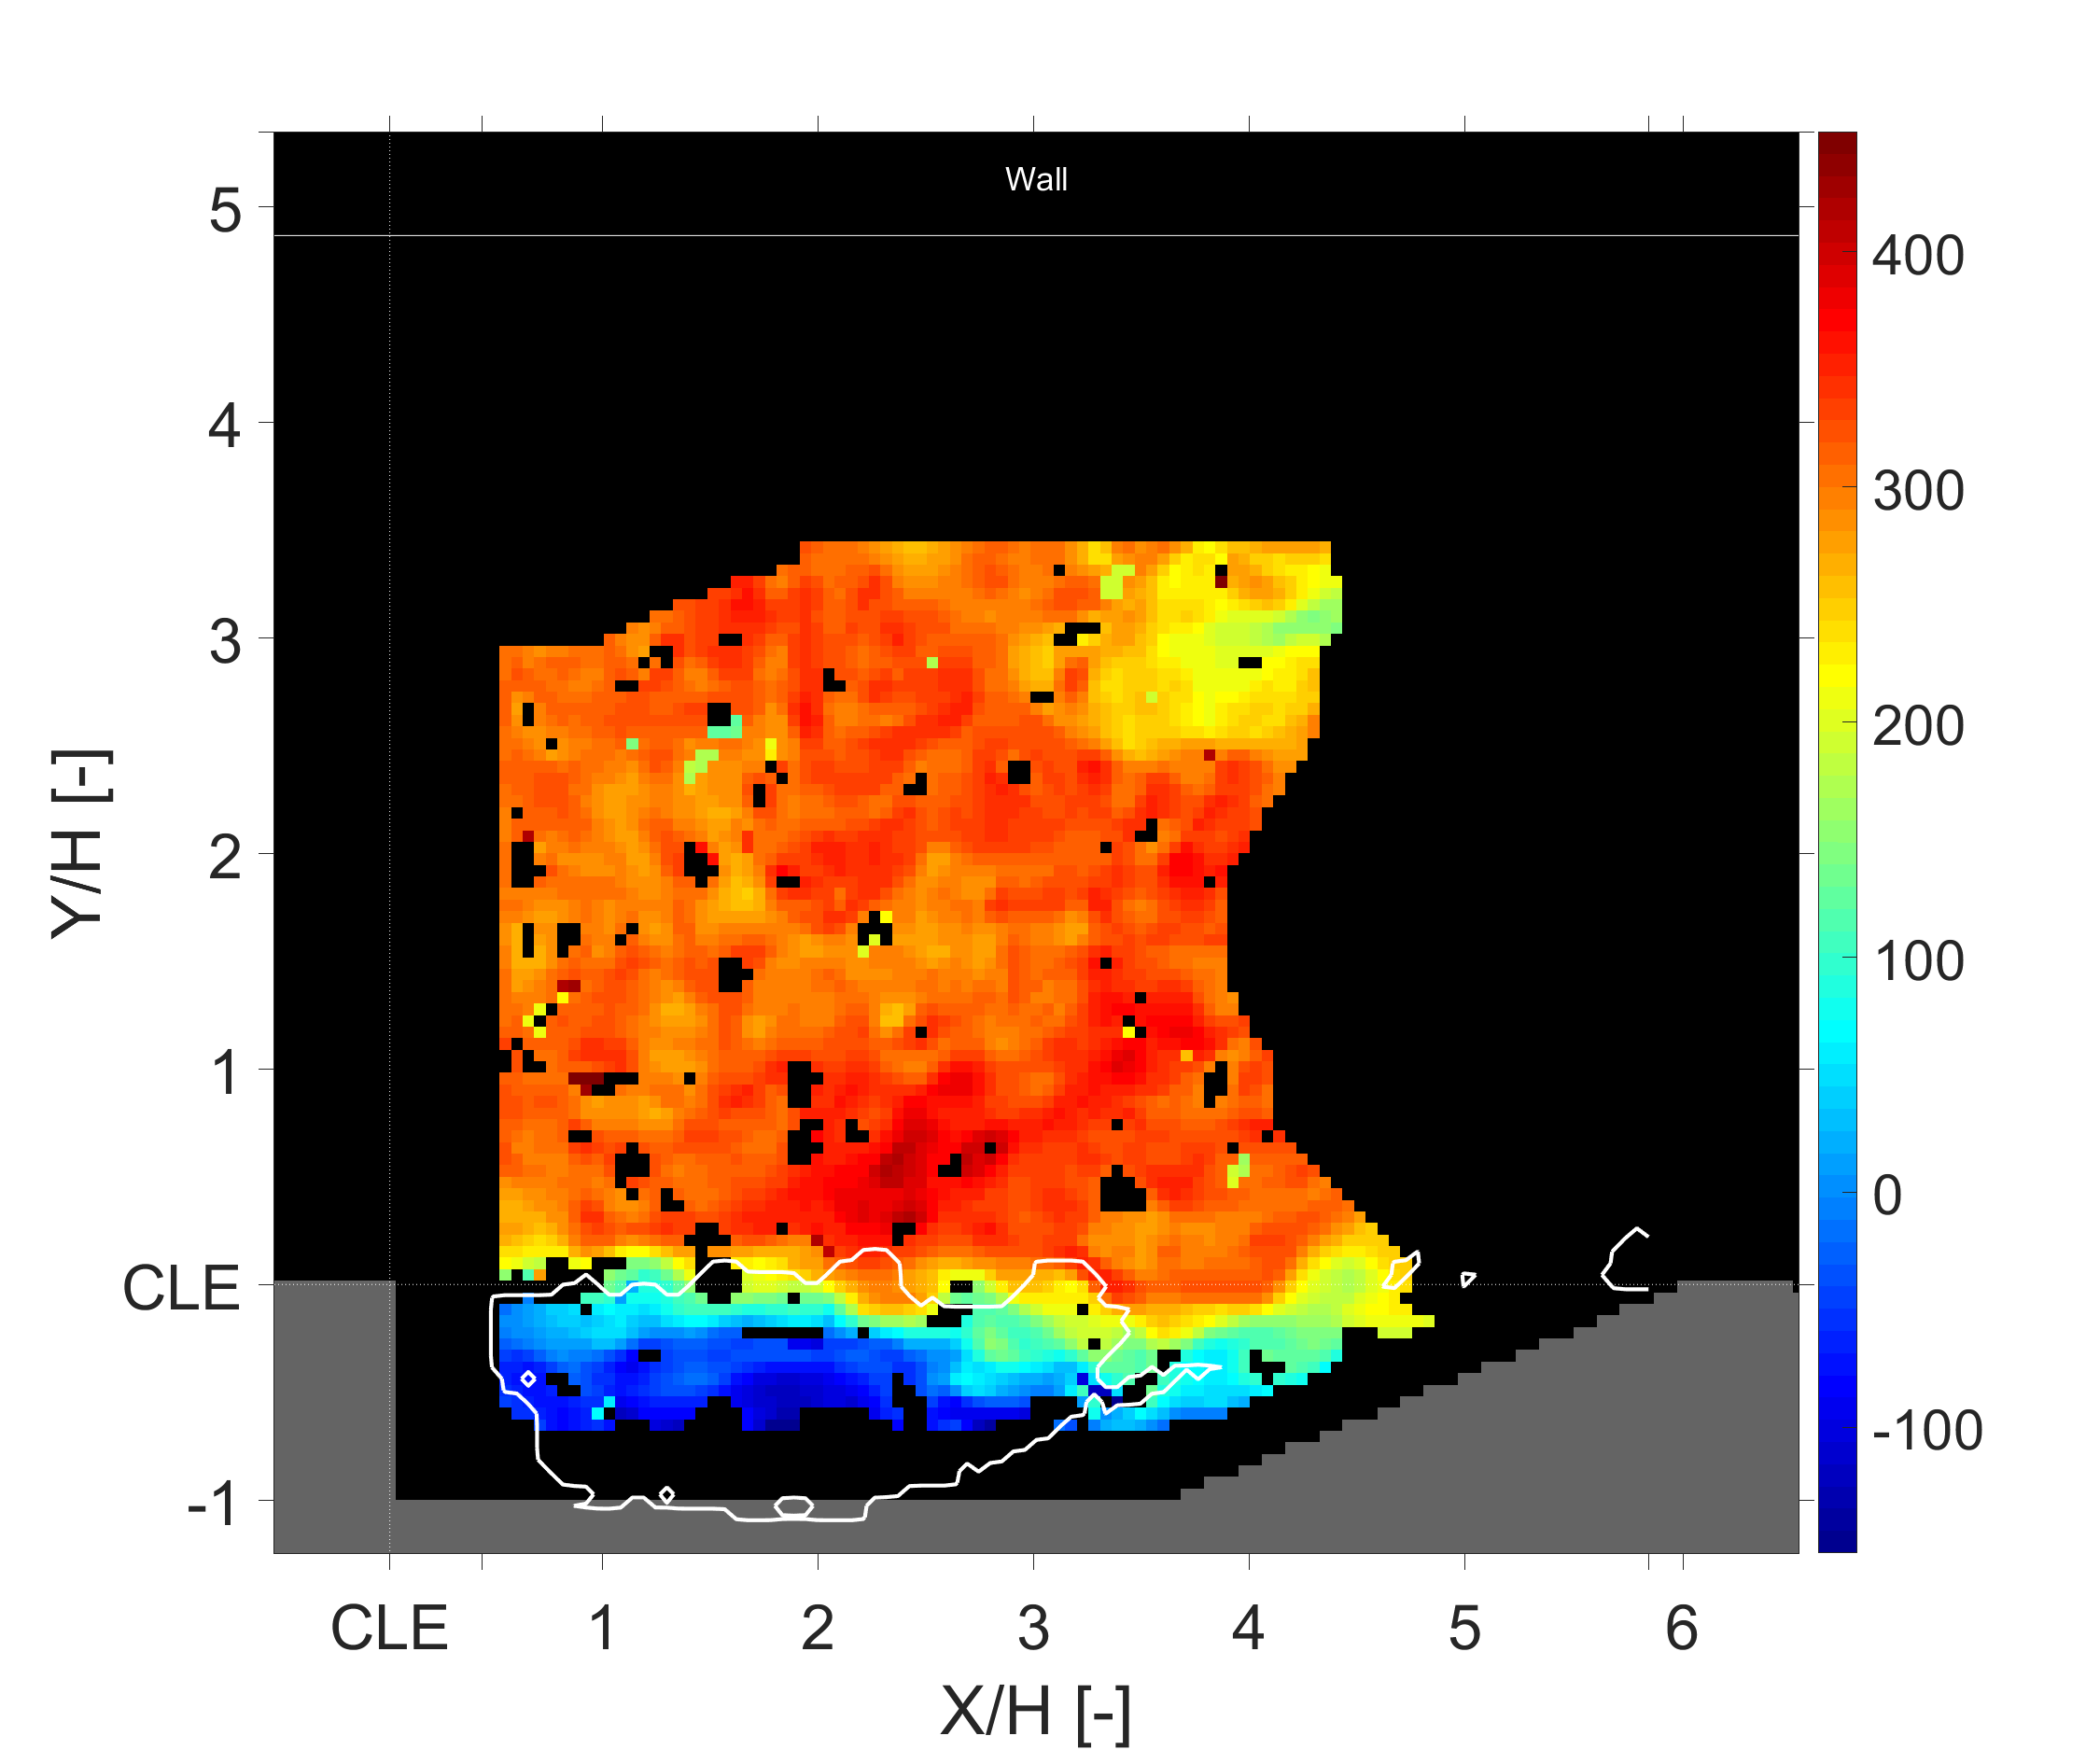
\includegraphics[height=2.5in, trim=0cm 0cm 0cm 0cm, clip]{figures/B1/combustion_instability/x/B1_Frame331_x}\hspace{0.5cm}} %pdfcrop
% \subcaptionbox{State 2\label{fig:B1_Frame2}}
%         {\hspace{0.5cm}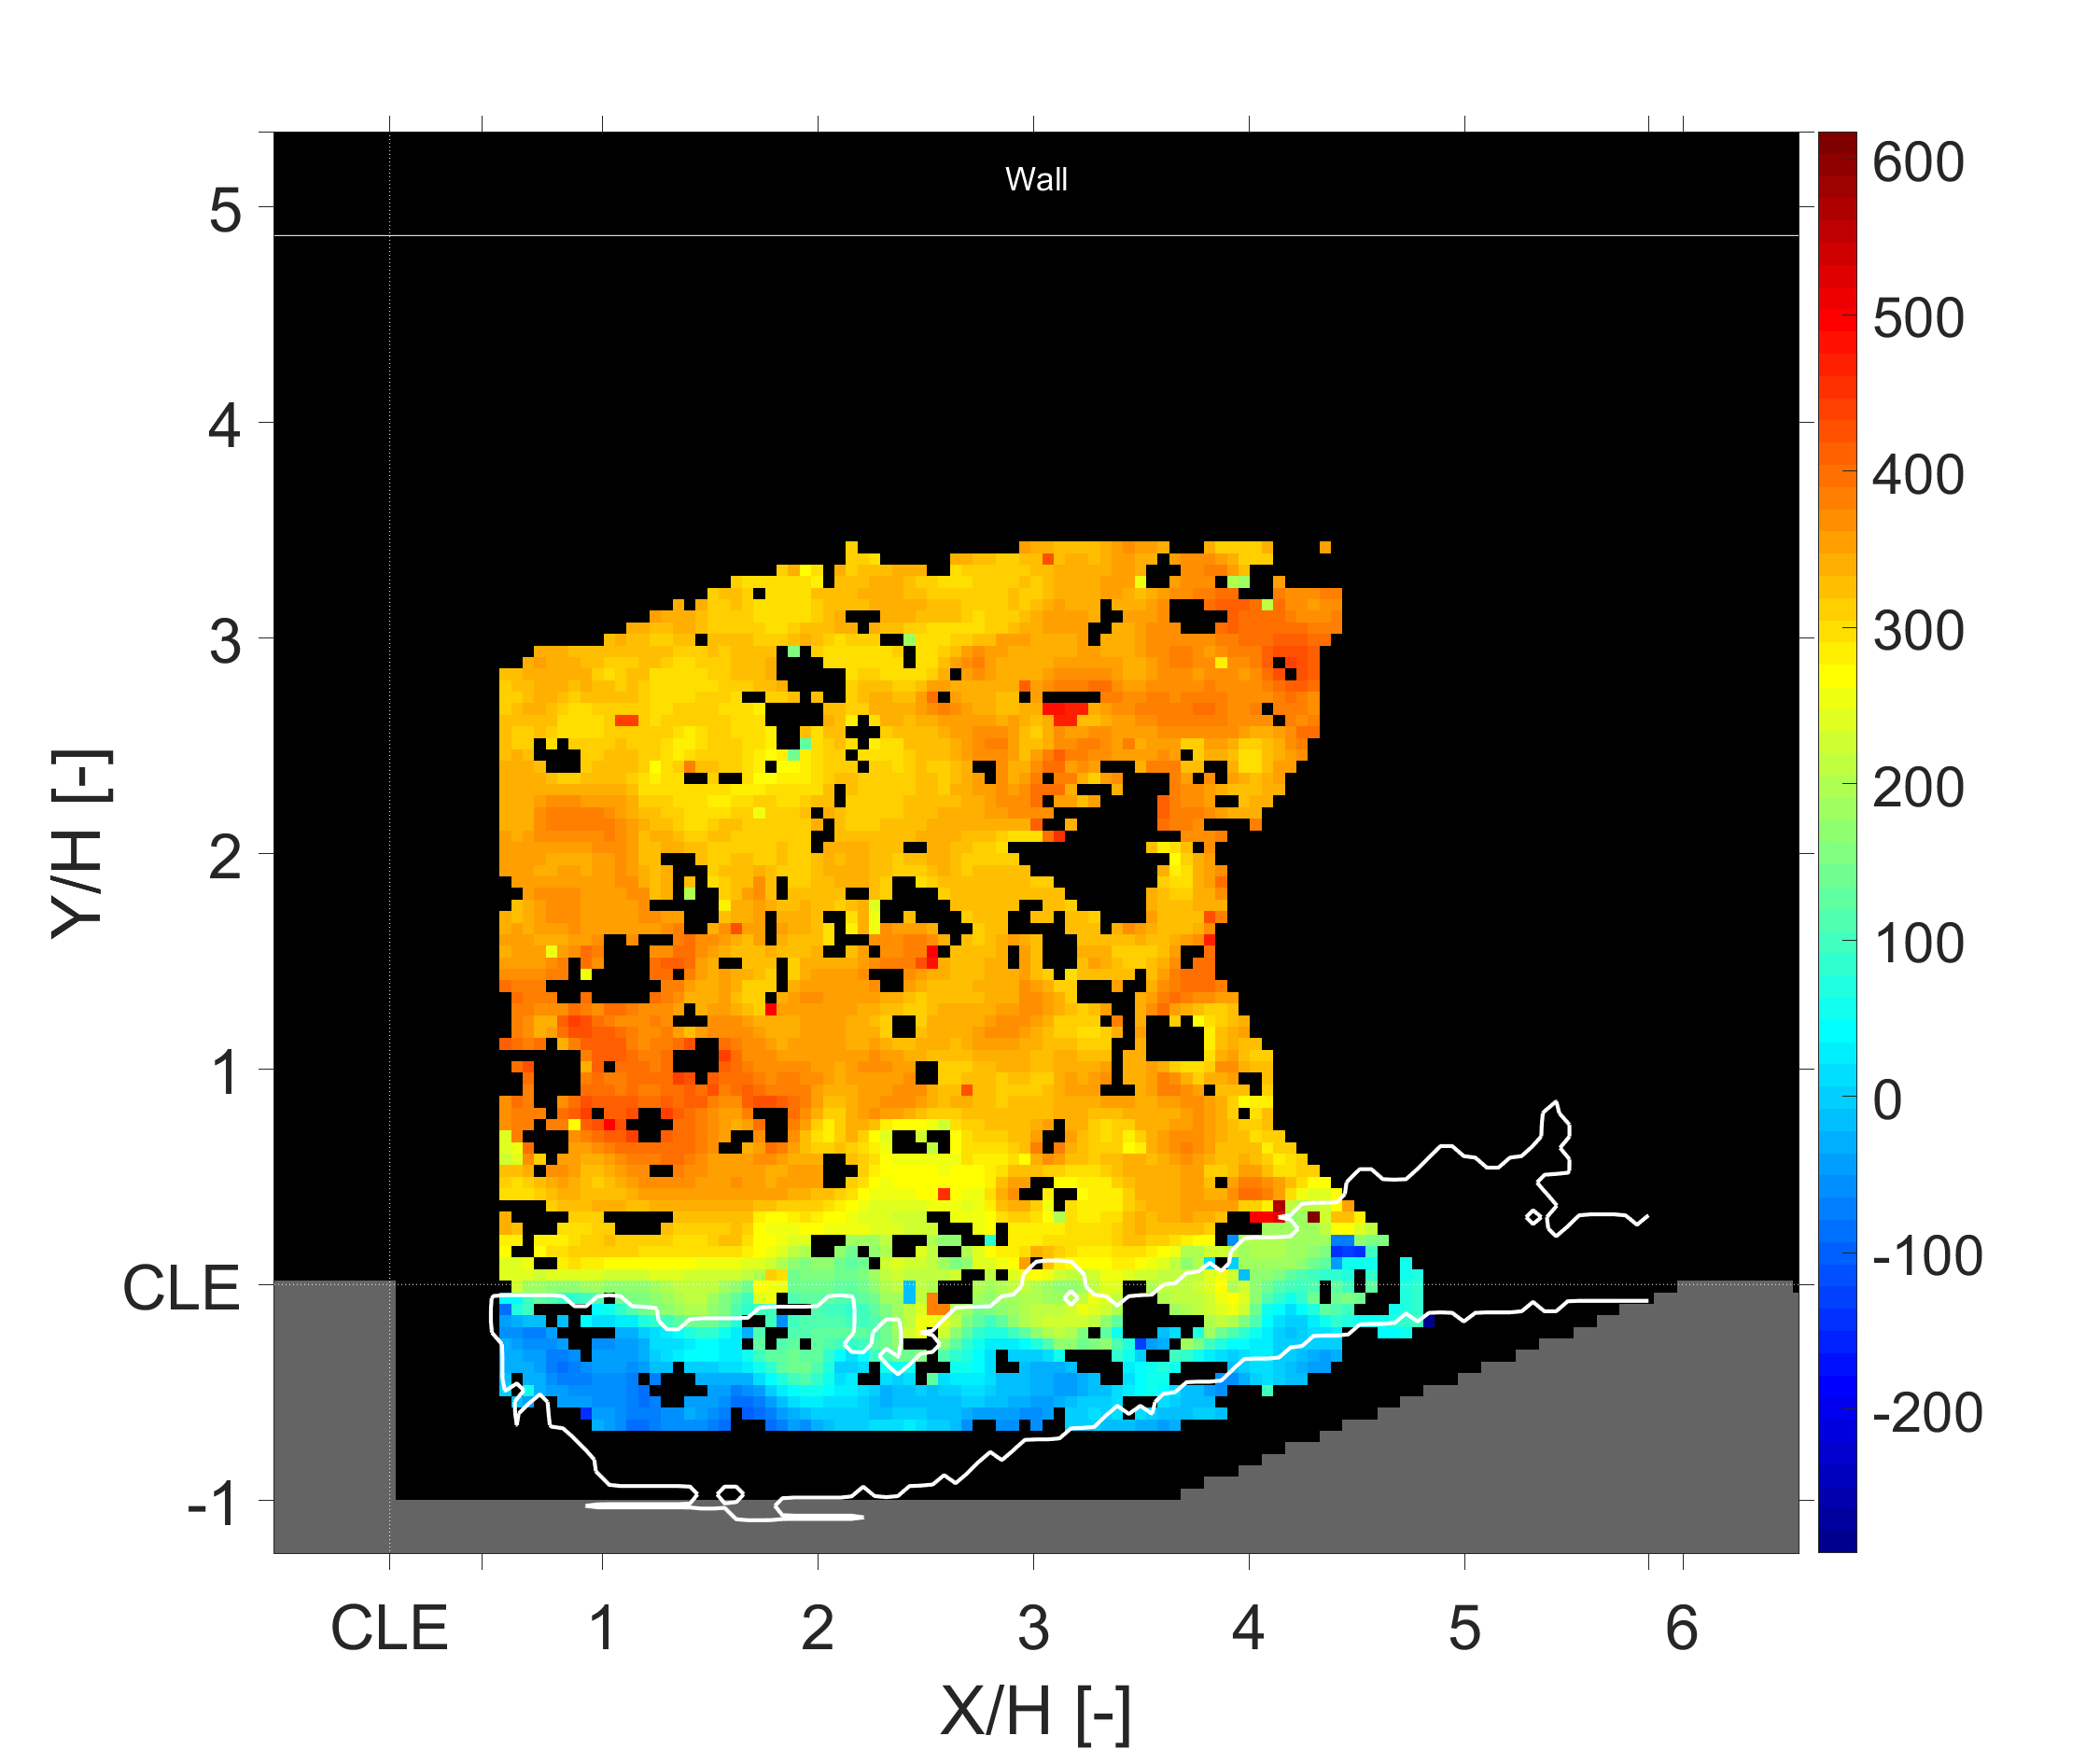
\includegraphics[height=2.5in, trim=0cm 0cm 0cm 0cm, clip]{figures/B1/combustion_instability/x/B1_Frame329_x}}
% \subcaptionbox{State 3\label{fig:B1_Frame3}}
%         {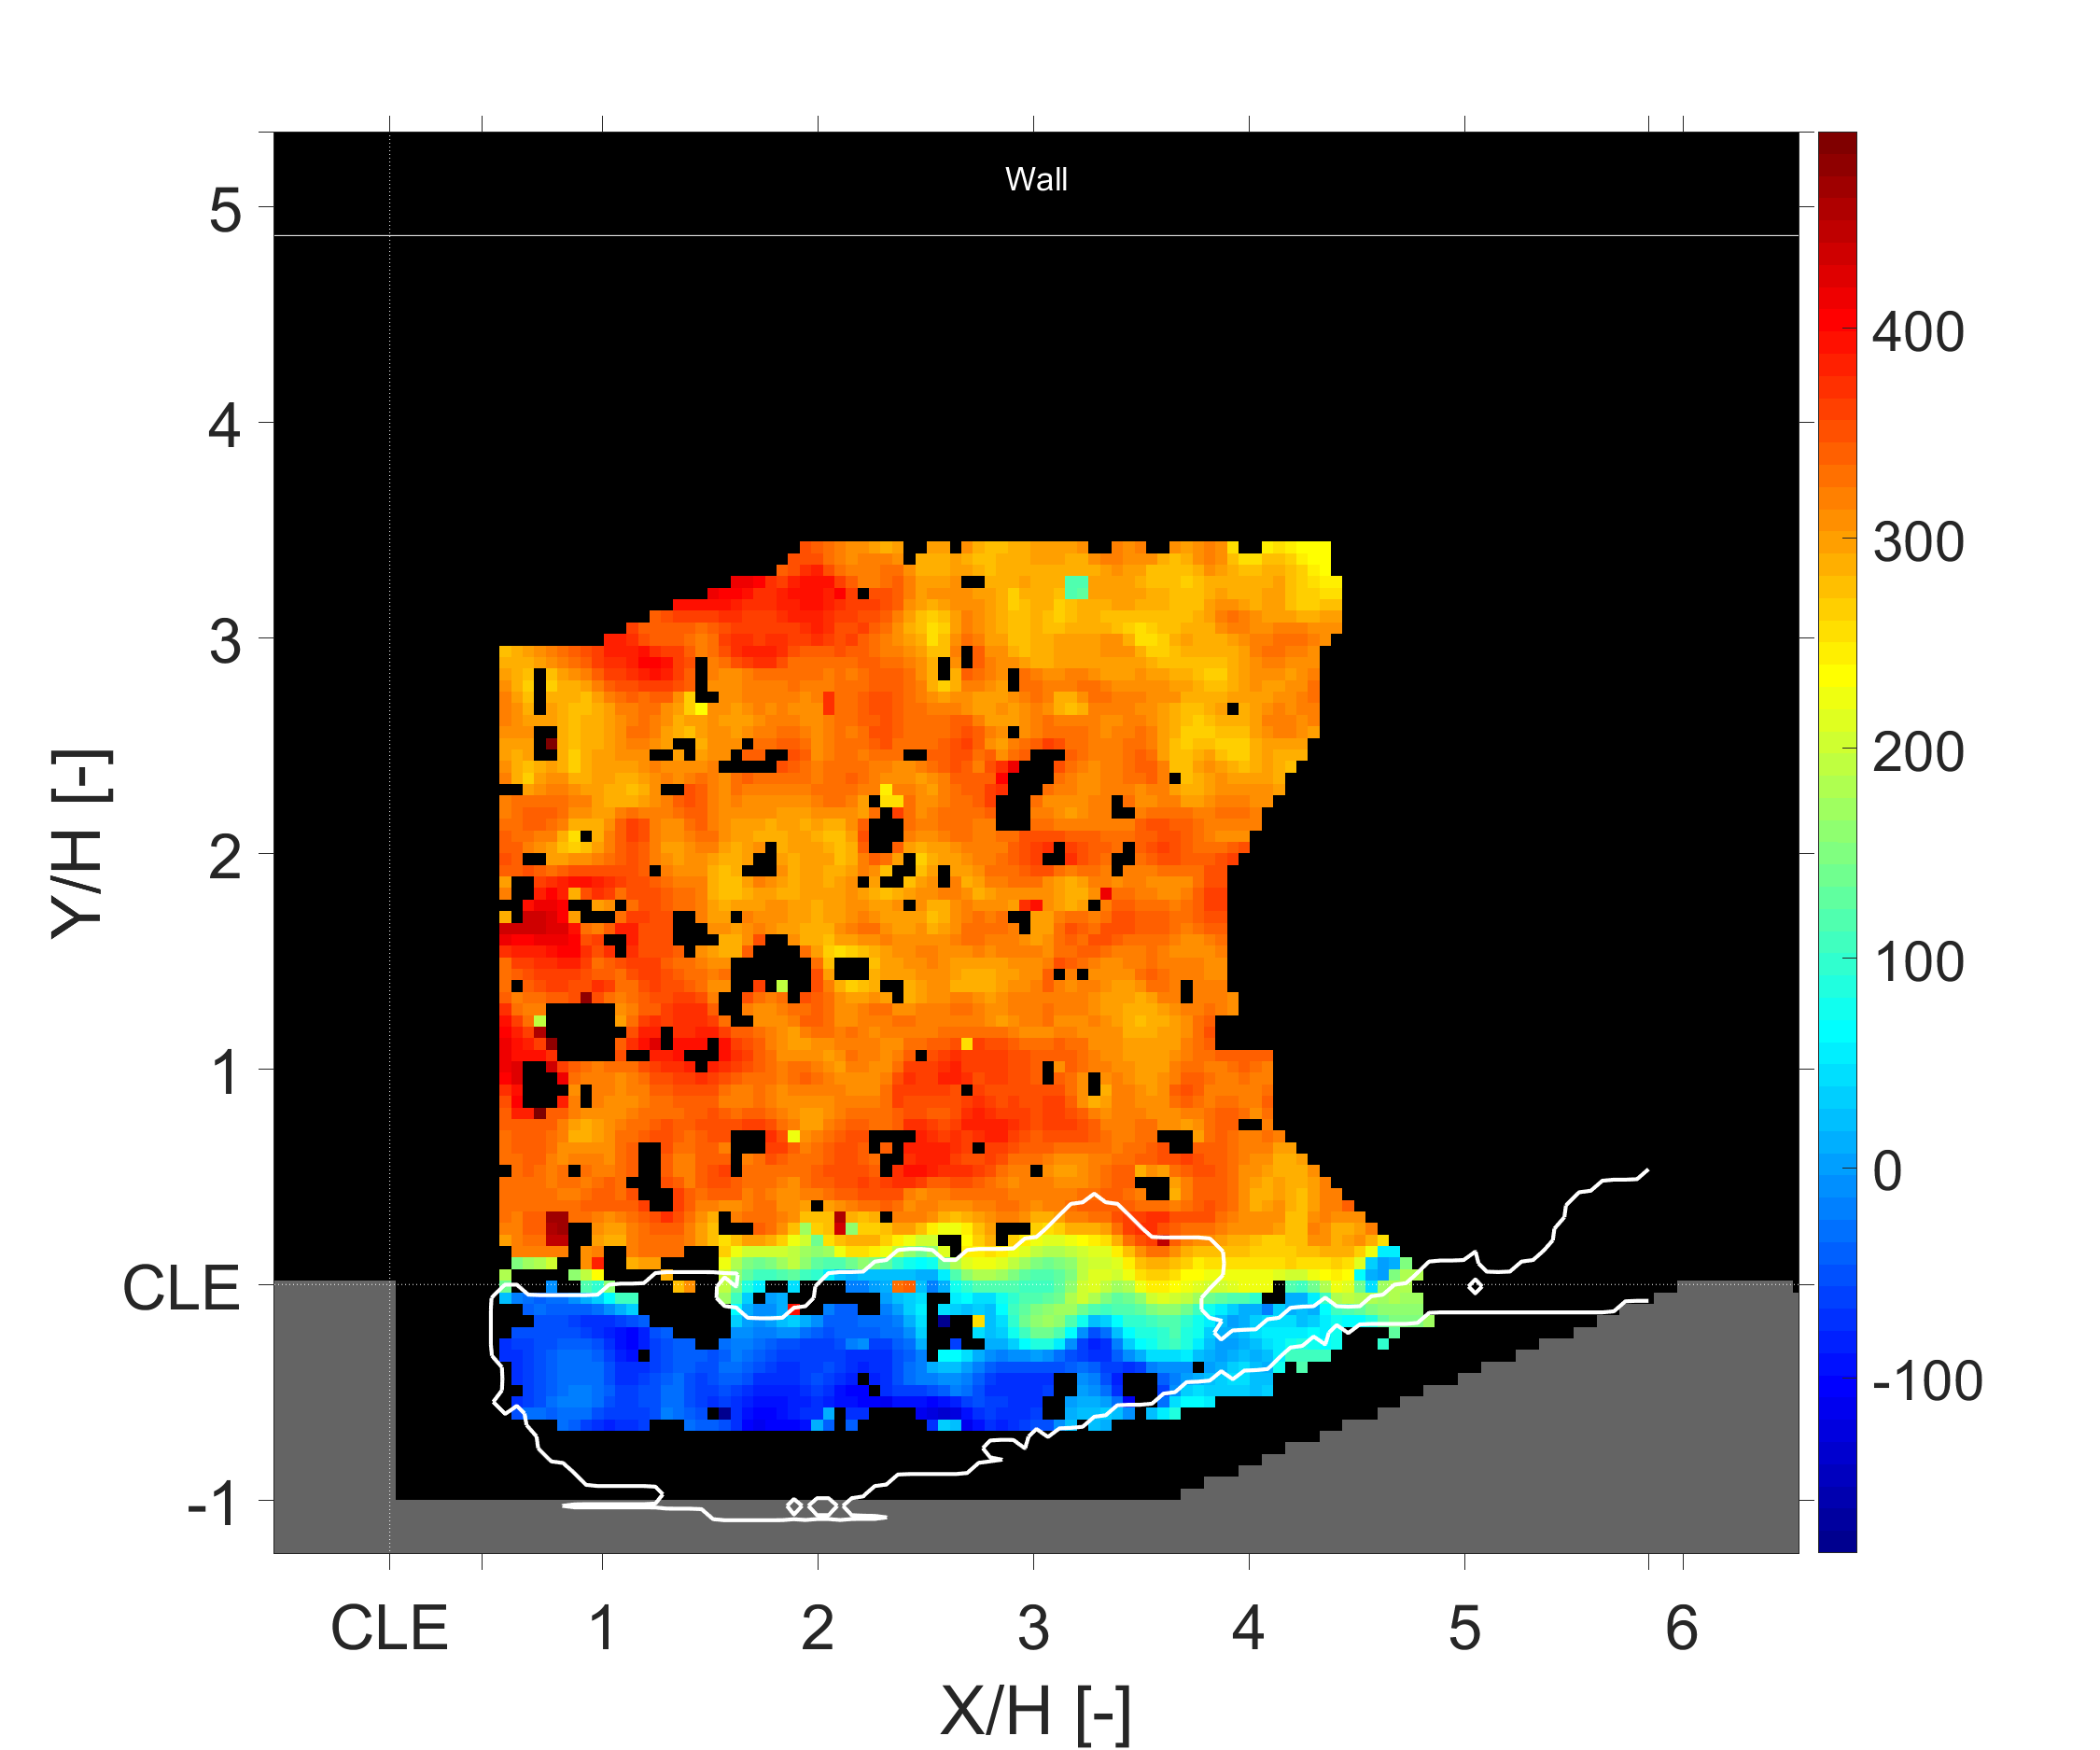
\includegraphics[height=2.5in, trim=0cm 0cm 0cm 0cm, clip]{figures/B1/combustion_instability/x/B1_Frame342_x}\hspace{0.5cm}}
% \subcaptionbox{State 4\label{fig:B1_Frame4}}
%         {\hspace{0.5cm}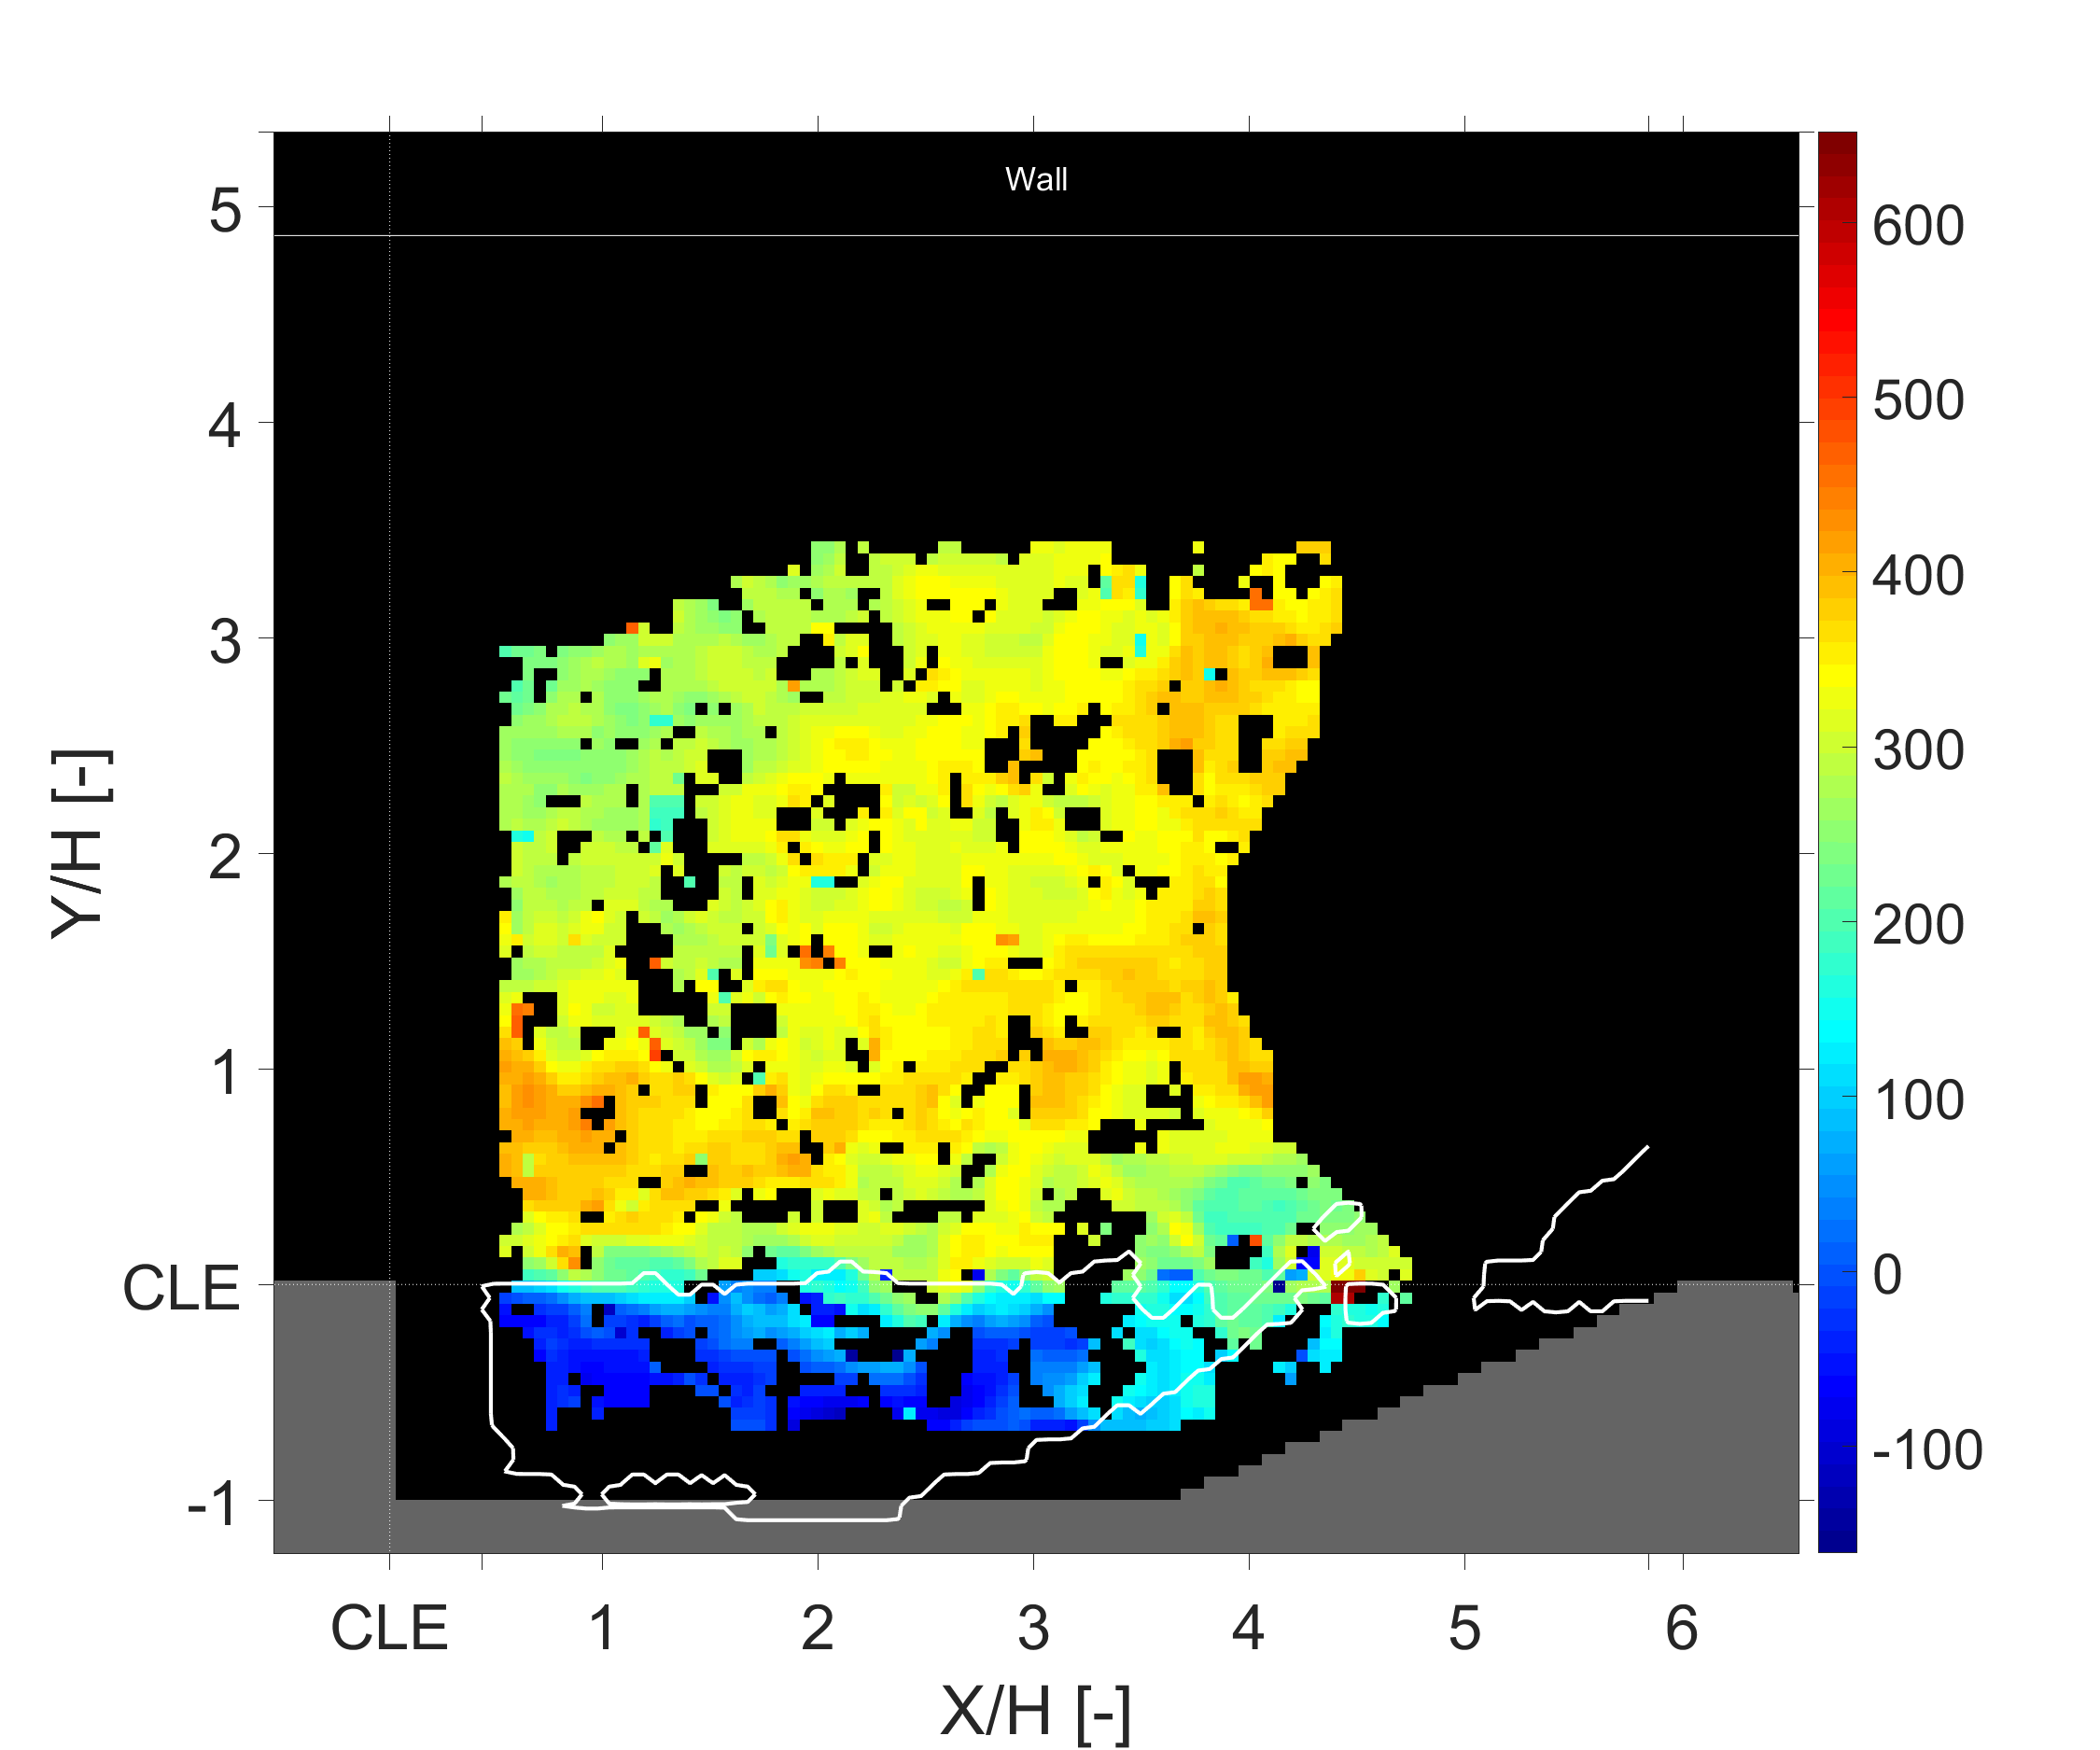
\includegraphics[height=2.5in, trim=0cm 0cm 0cm 0cm, clip]{figures/B1/combustion_instability/x/B1_Frame339_x}}
% \subcaptionbox{State 5\label{fig:B1_Frame5}}
%         {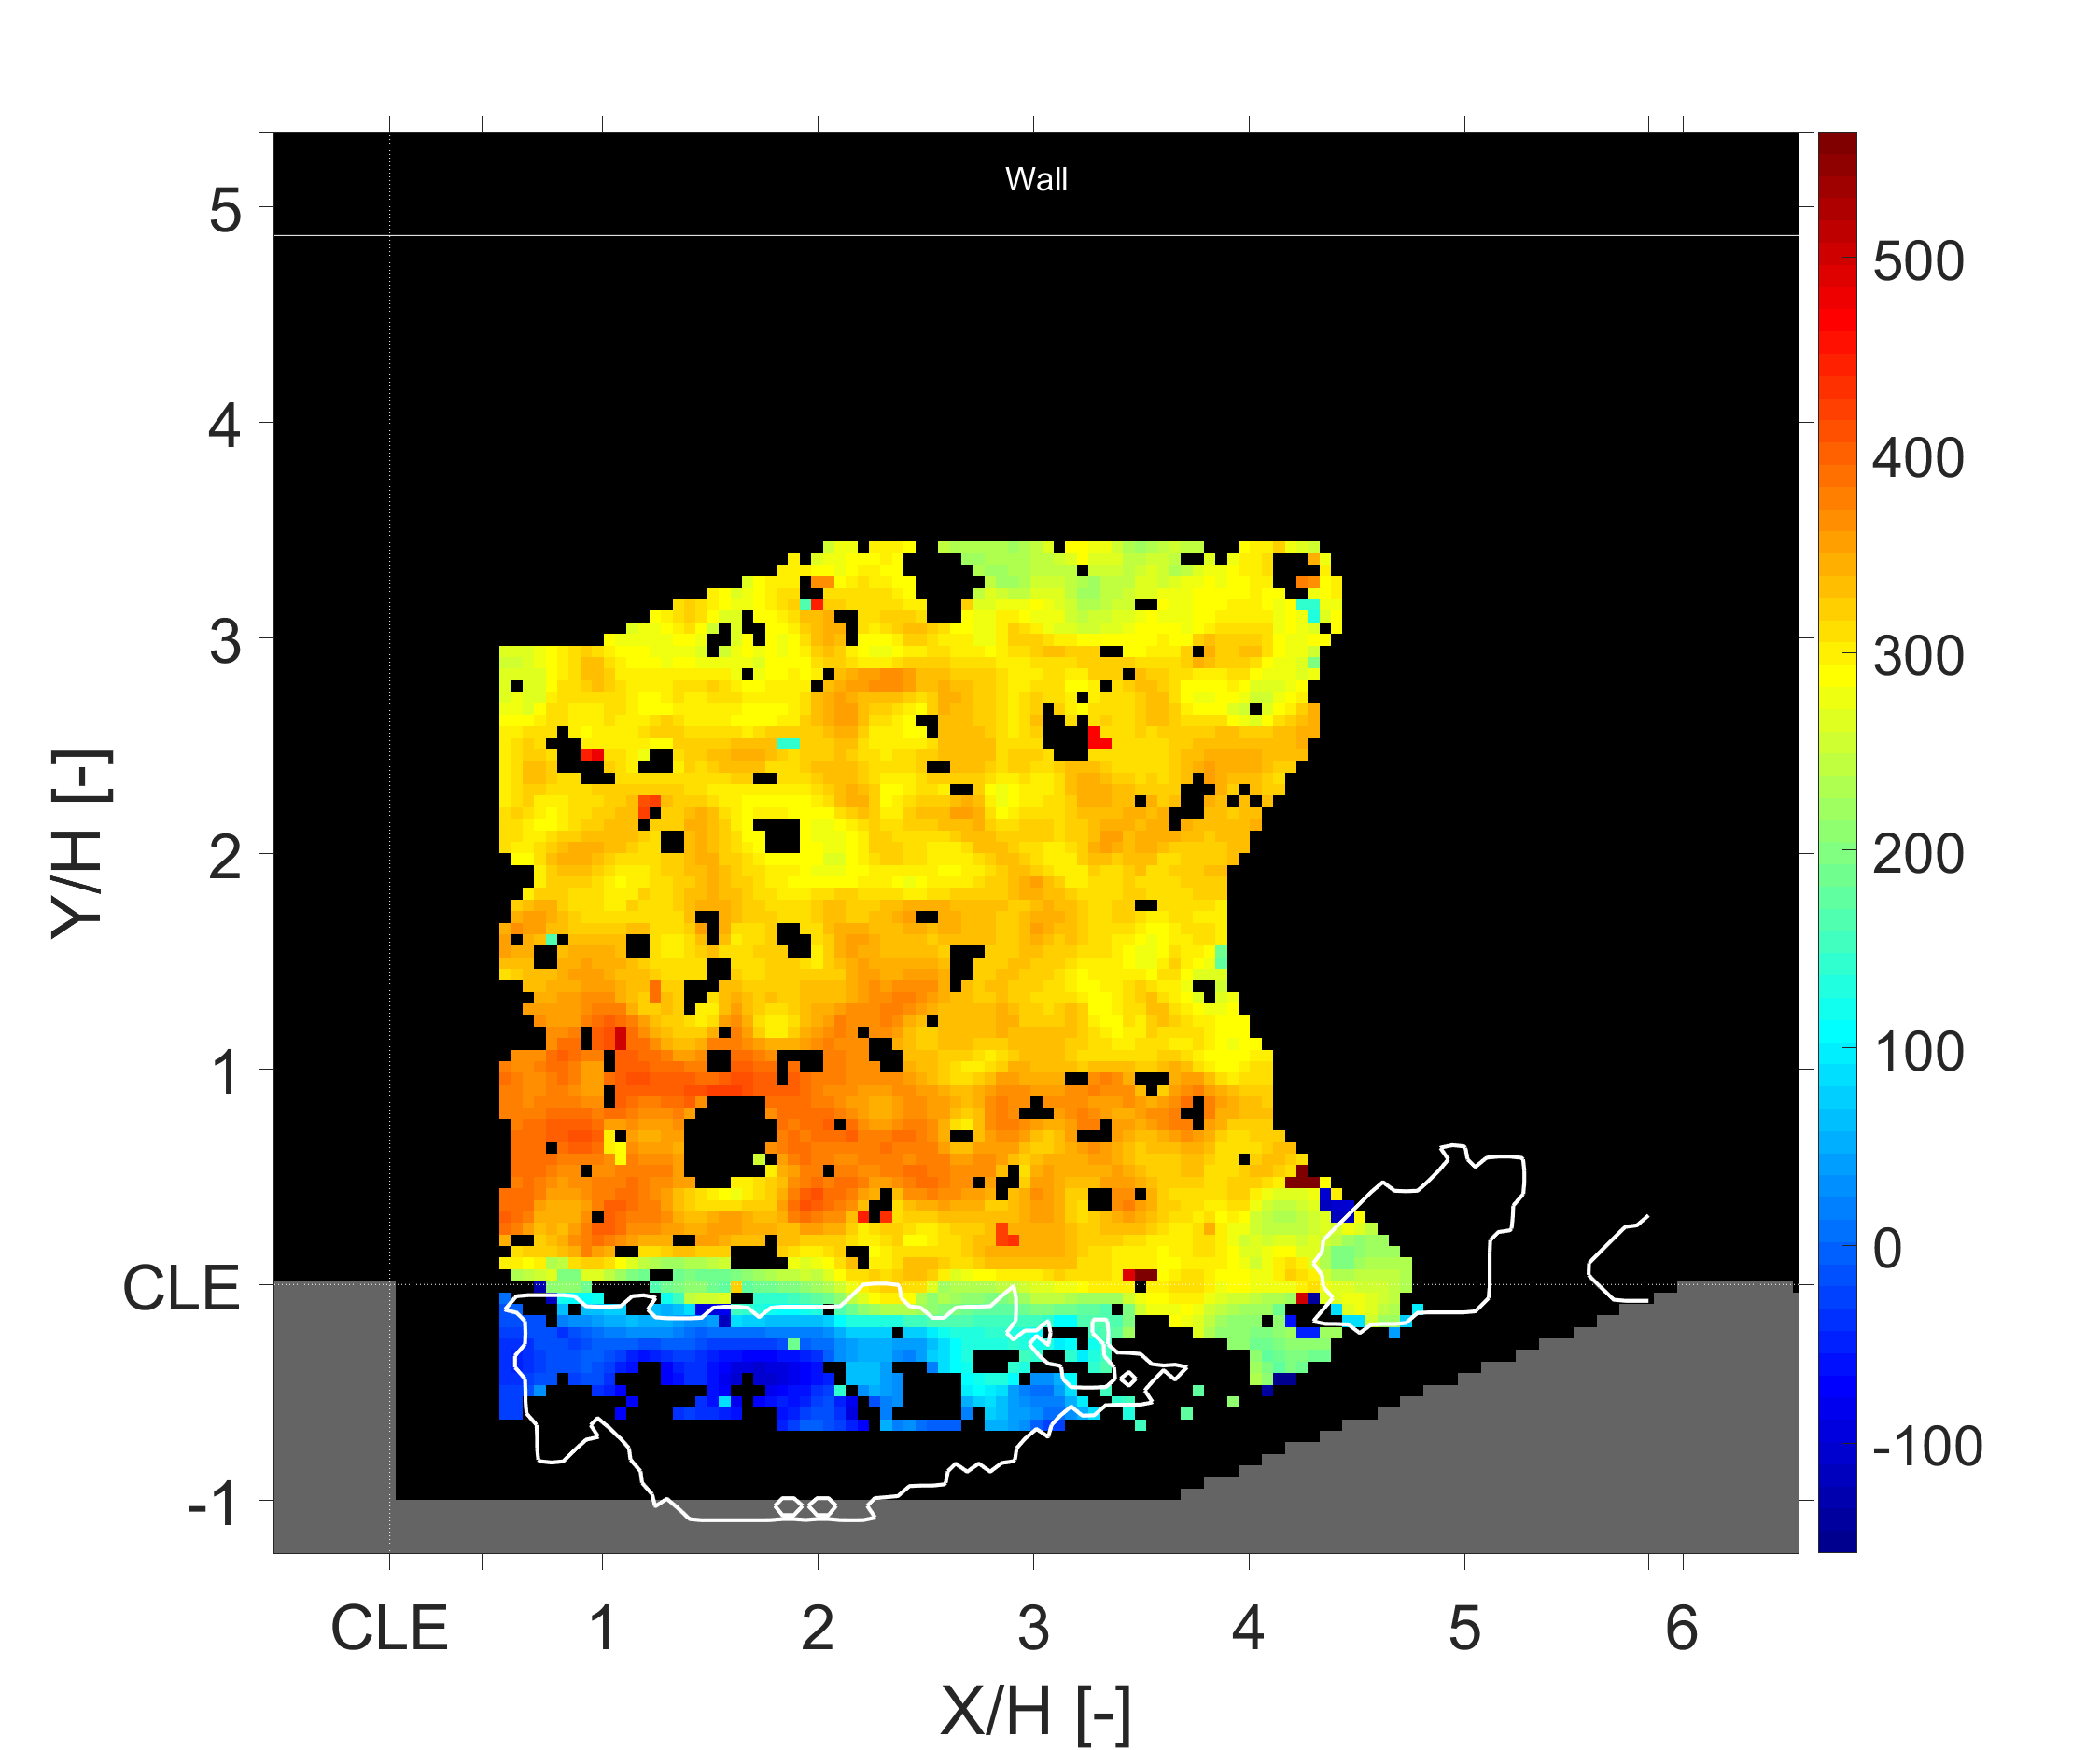
\includegraphics[height=2.5in, trim=0cm 0cm 0cm 0cm, clip]{figures/B1/combustion_instability/x/B1_Frame306_x.png}\hspace{0.5cm}}
%         \subcaptionbox{State 2 with duct velocities below average\label{fig:B1_Frame6}}
%         {\hspace{0.5cm}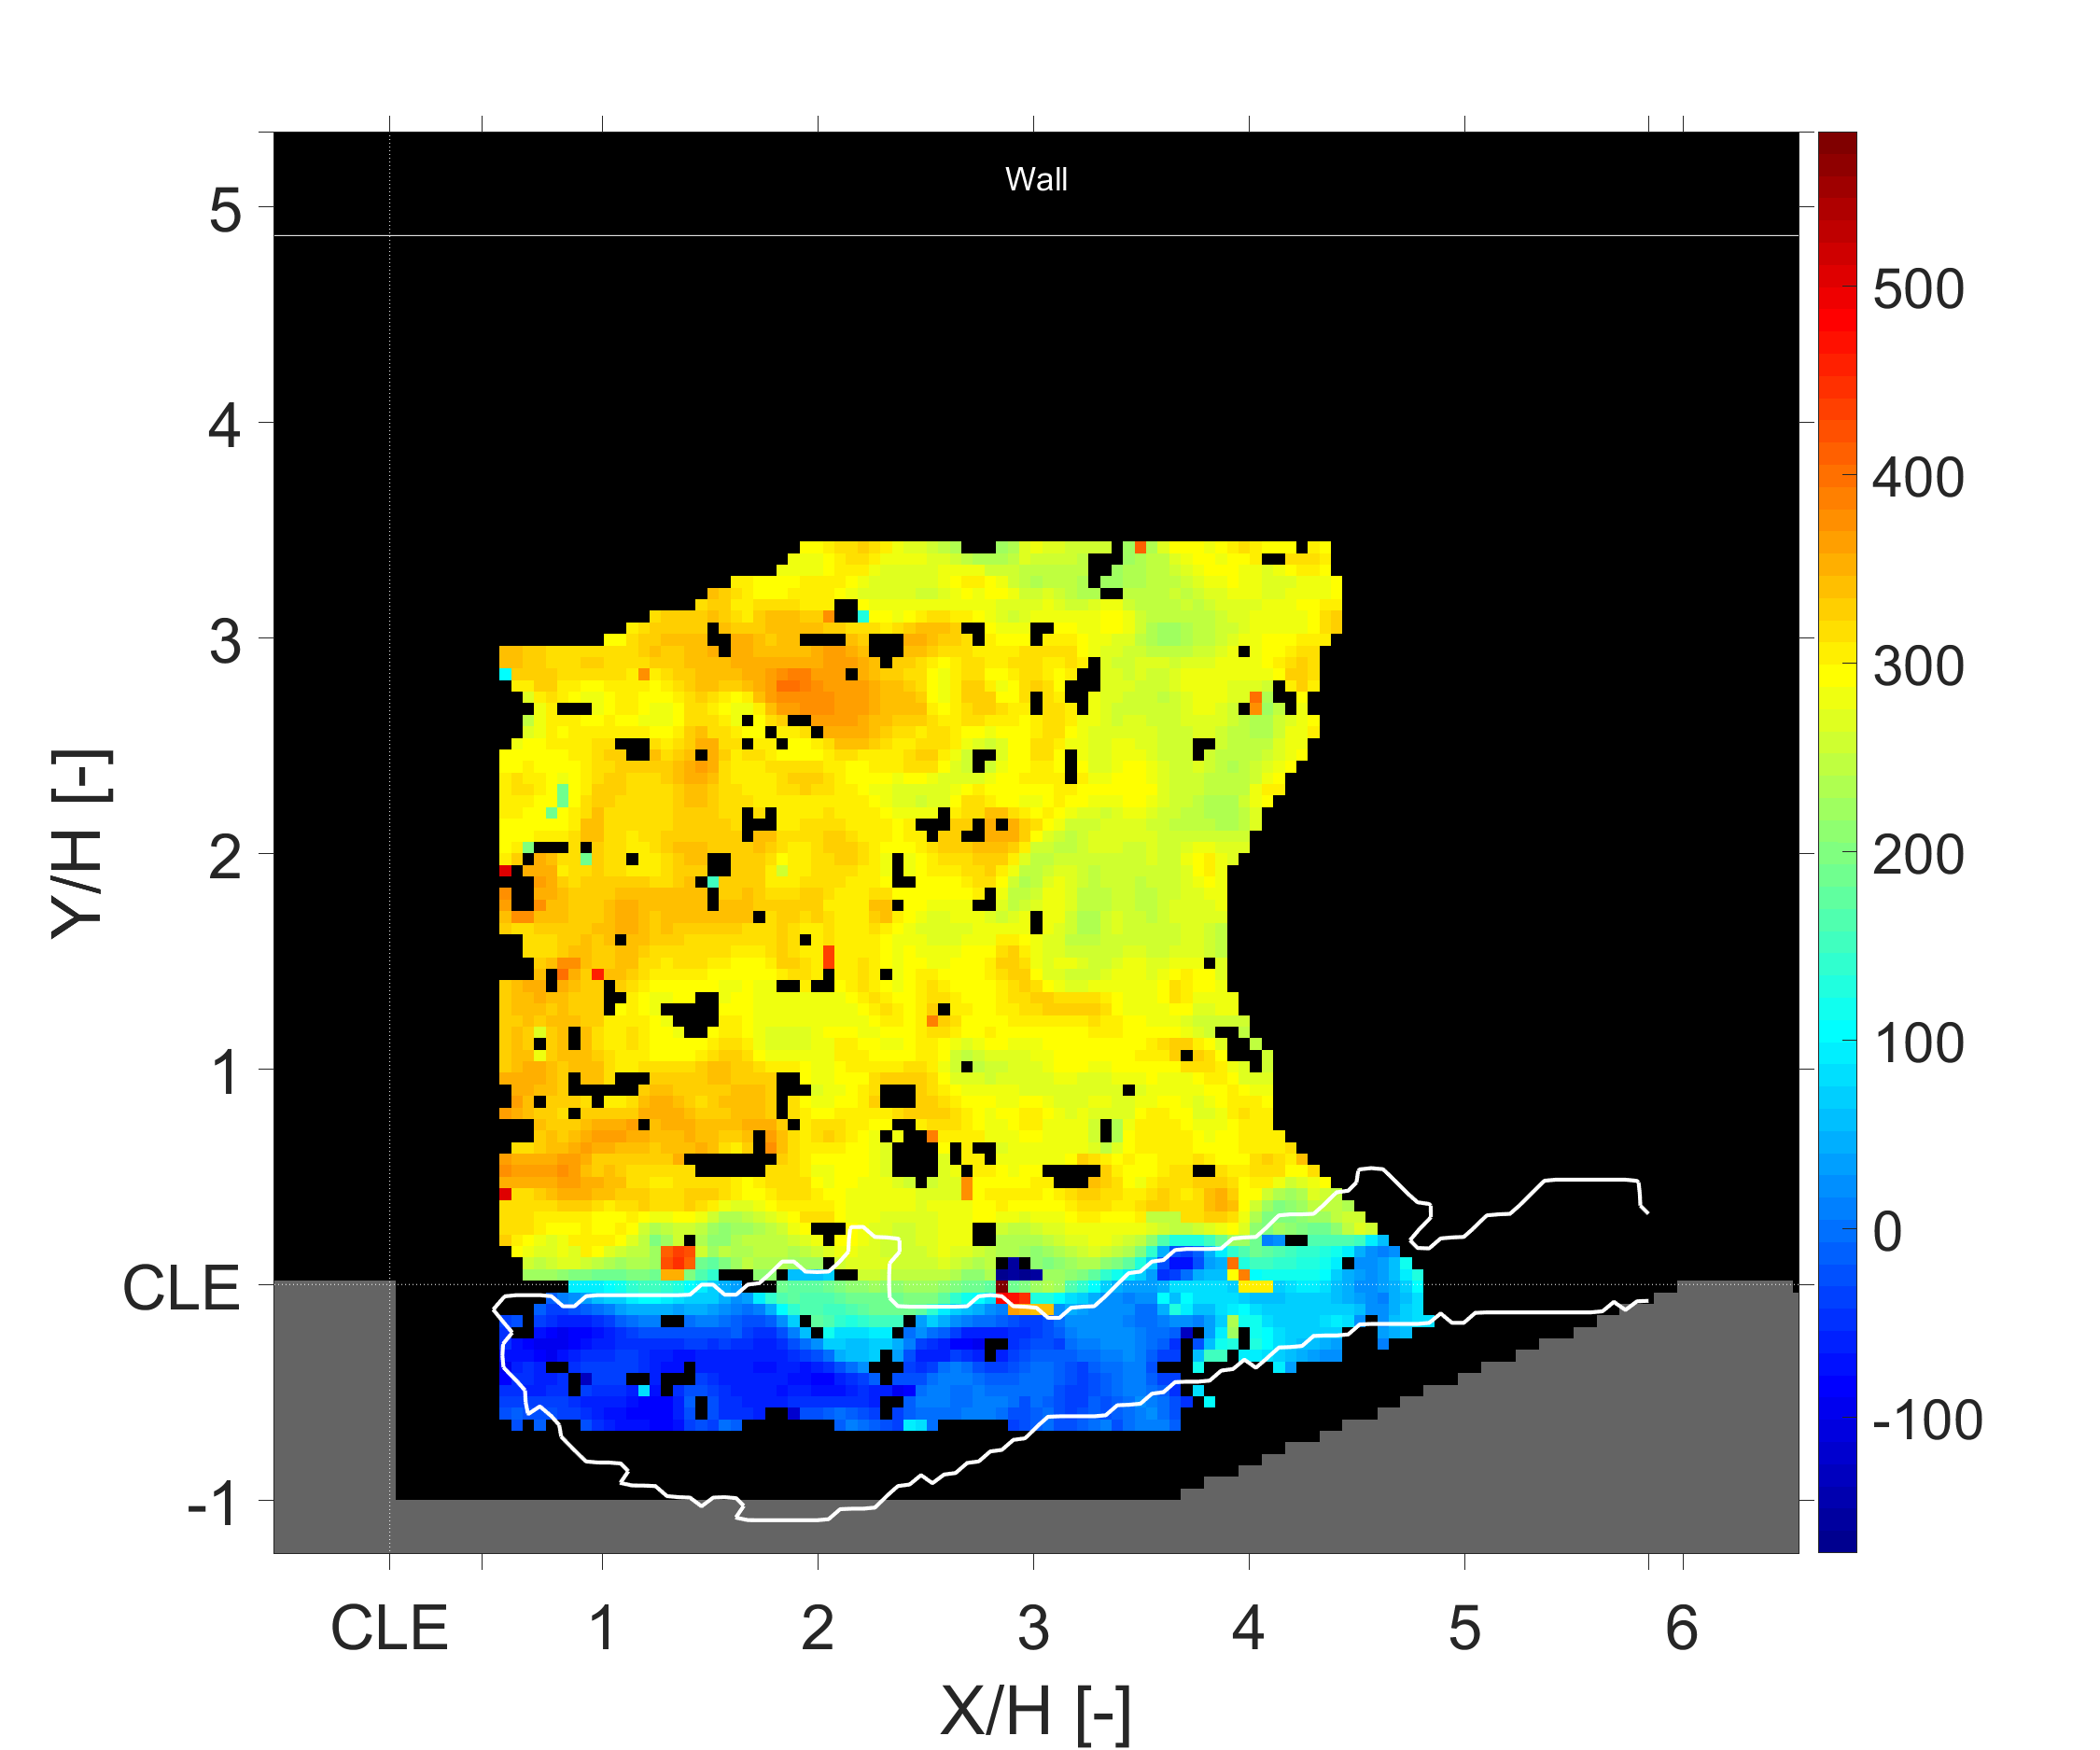
\includegraphics[height=2.5in, trim=0cm 0cm 0cm 0cm, clip]{figures/B1/combustion_instability/x/B1_Frame301_x}}
% \caption{$U_x$, select instantaneous PIV-PLIF frames.}\label{fig:ch3_inst_B1}
% \end{figure}

% \begin{figure}
% \centering
% \subcaptionbox{State 1\label{fig:B1_Frame1y}}
%         {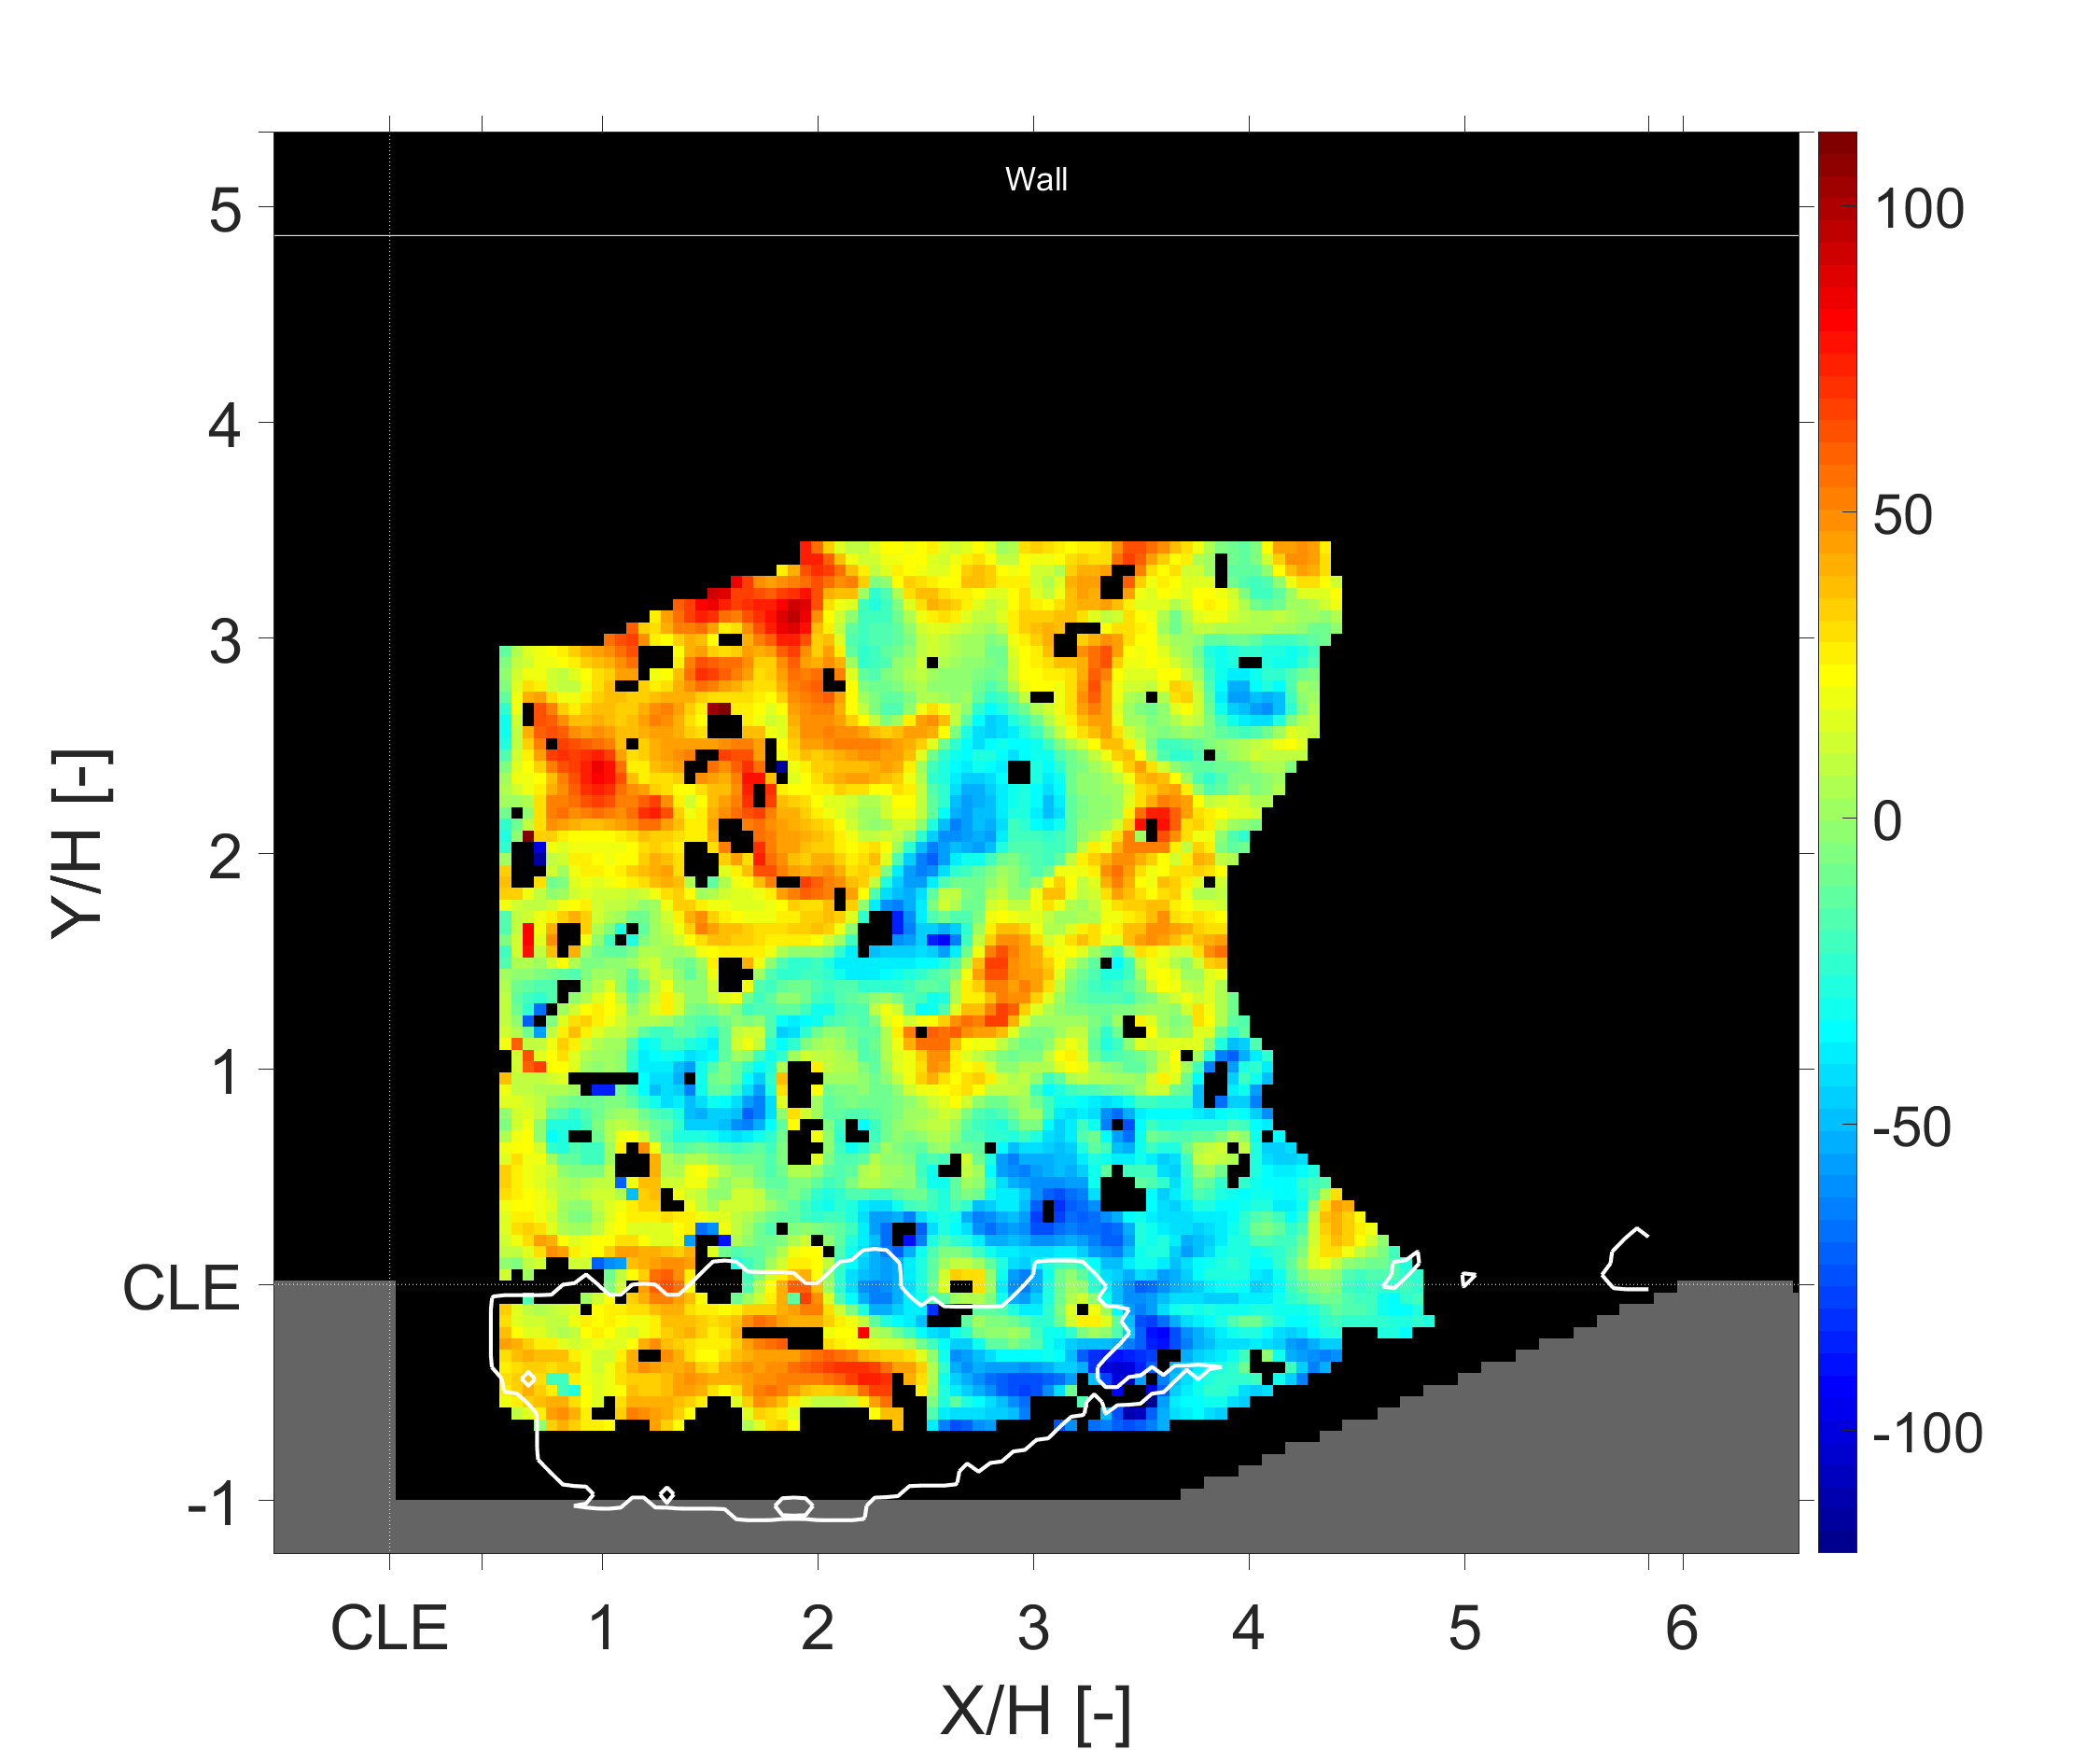
\includegraphics[height=2.5in, trim=0cm 0cm 0cm 0cm, clip]{figures/B1/combustion_instability/y/B1_Frame331_y}\hspace{0.5cm}} %pdfcrop
% \subcaptionbox{State 2\label{fig:B1_Frame2y}}
%         {\hspace{0.5cm}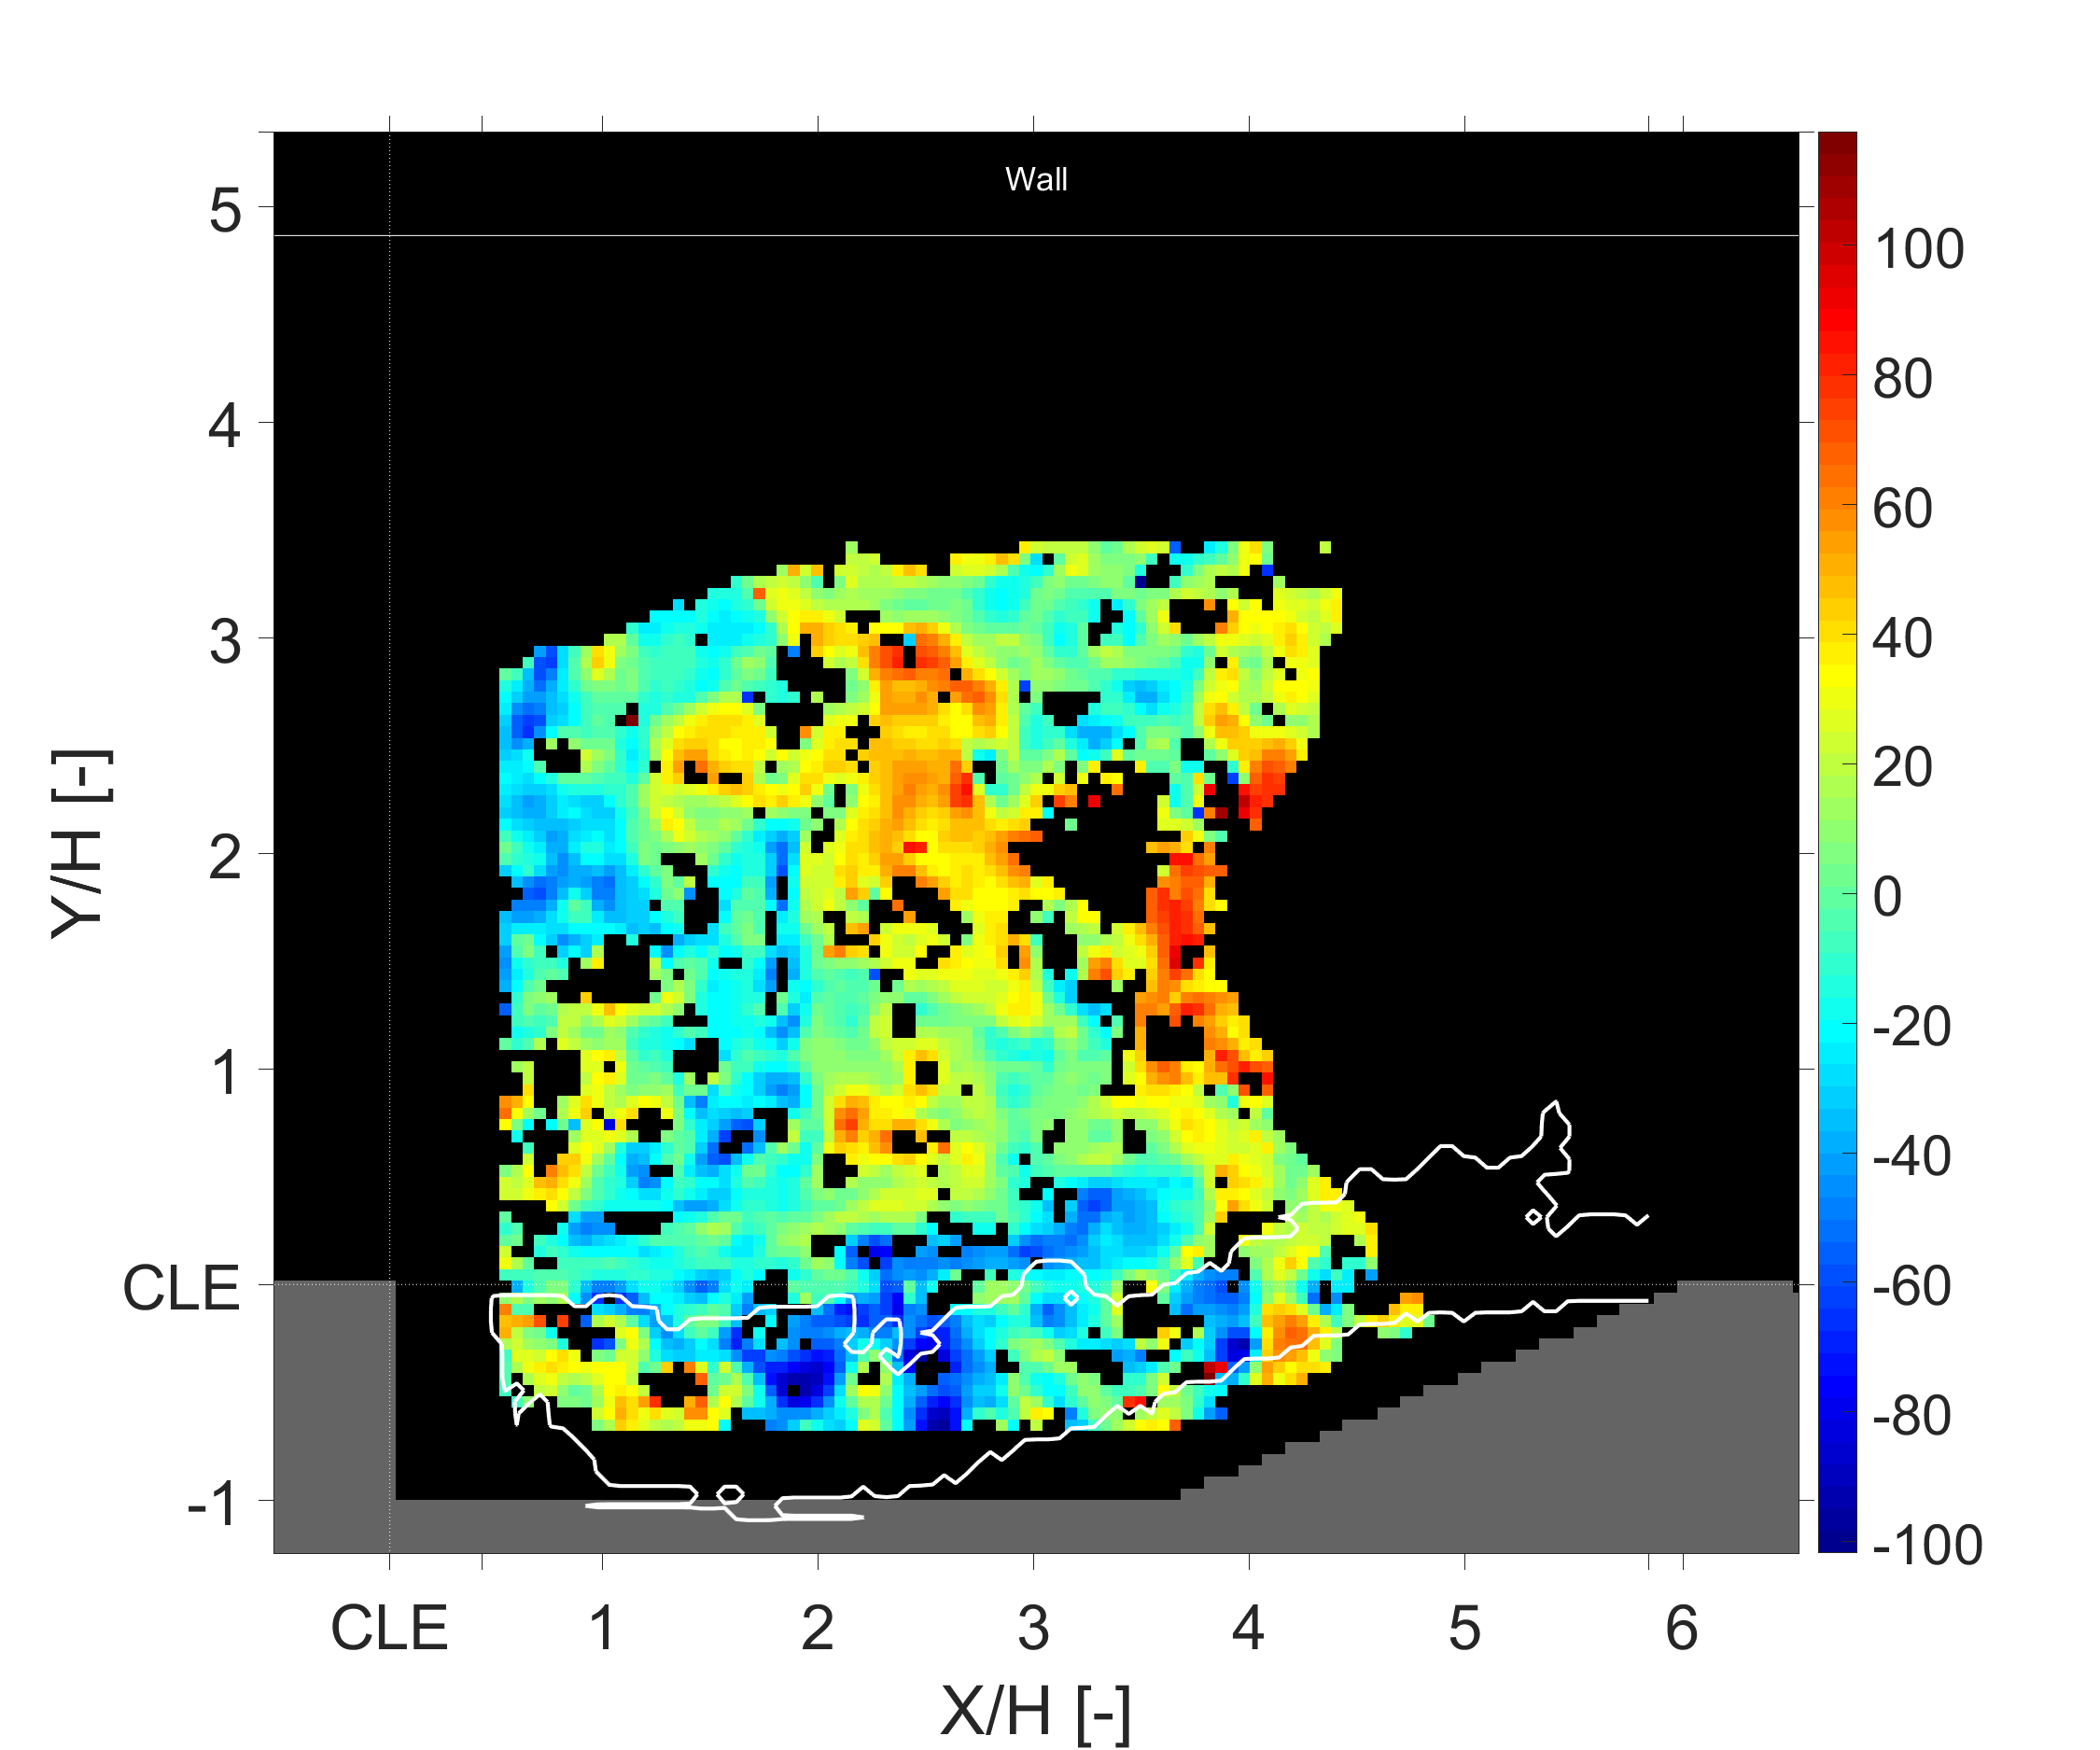
\includegraphics[height=2.5in, trim=0cm 0cm 0cm 0cm, clip]{figures/B1/combustion_instability/y/B1_Frame329_y}}
% \subcaptionbox{State 3\label{fig:B1_Frame3y}}
%         {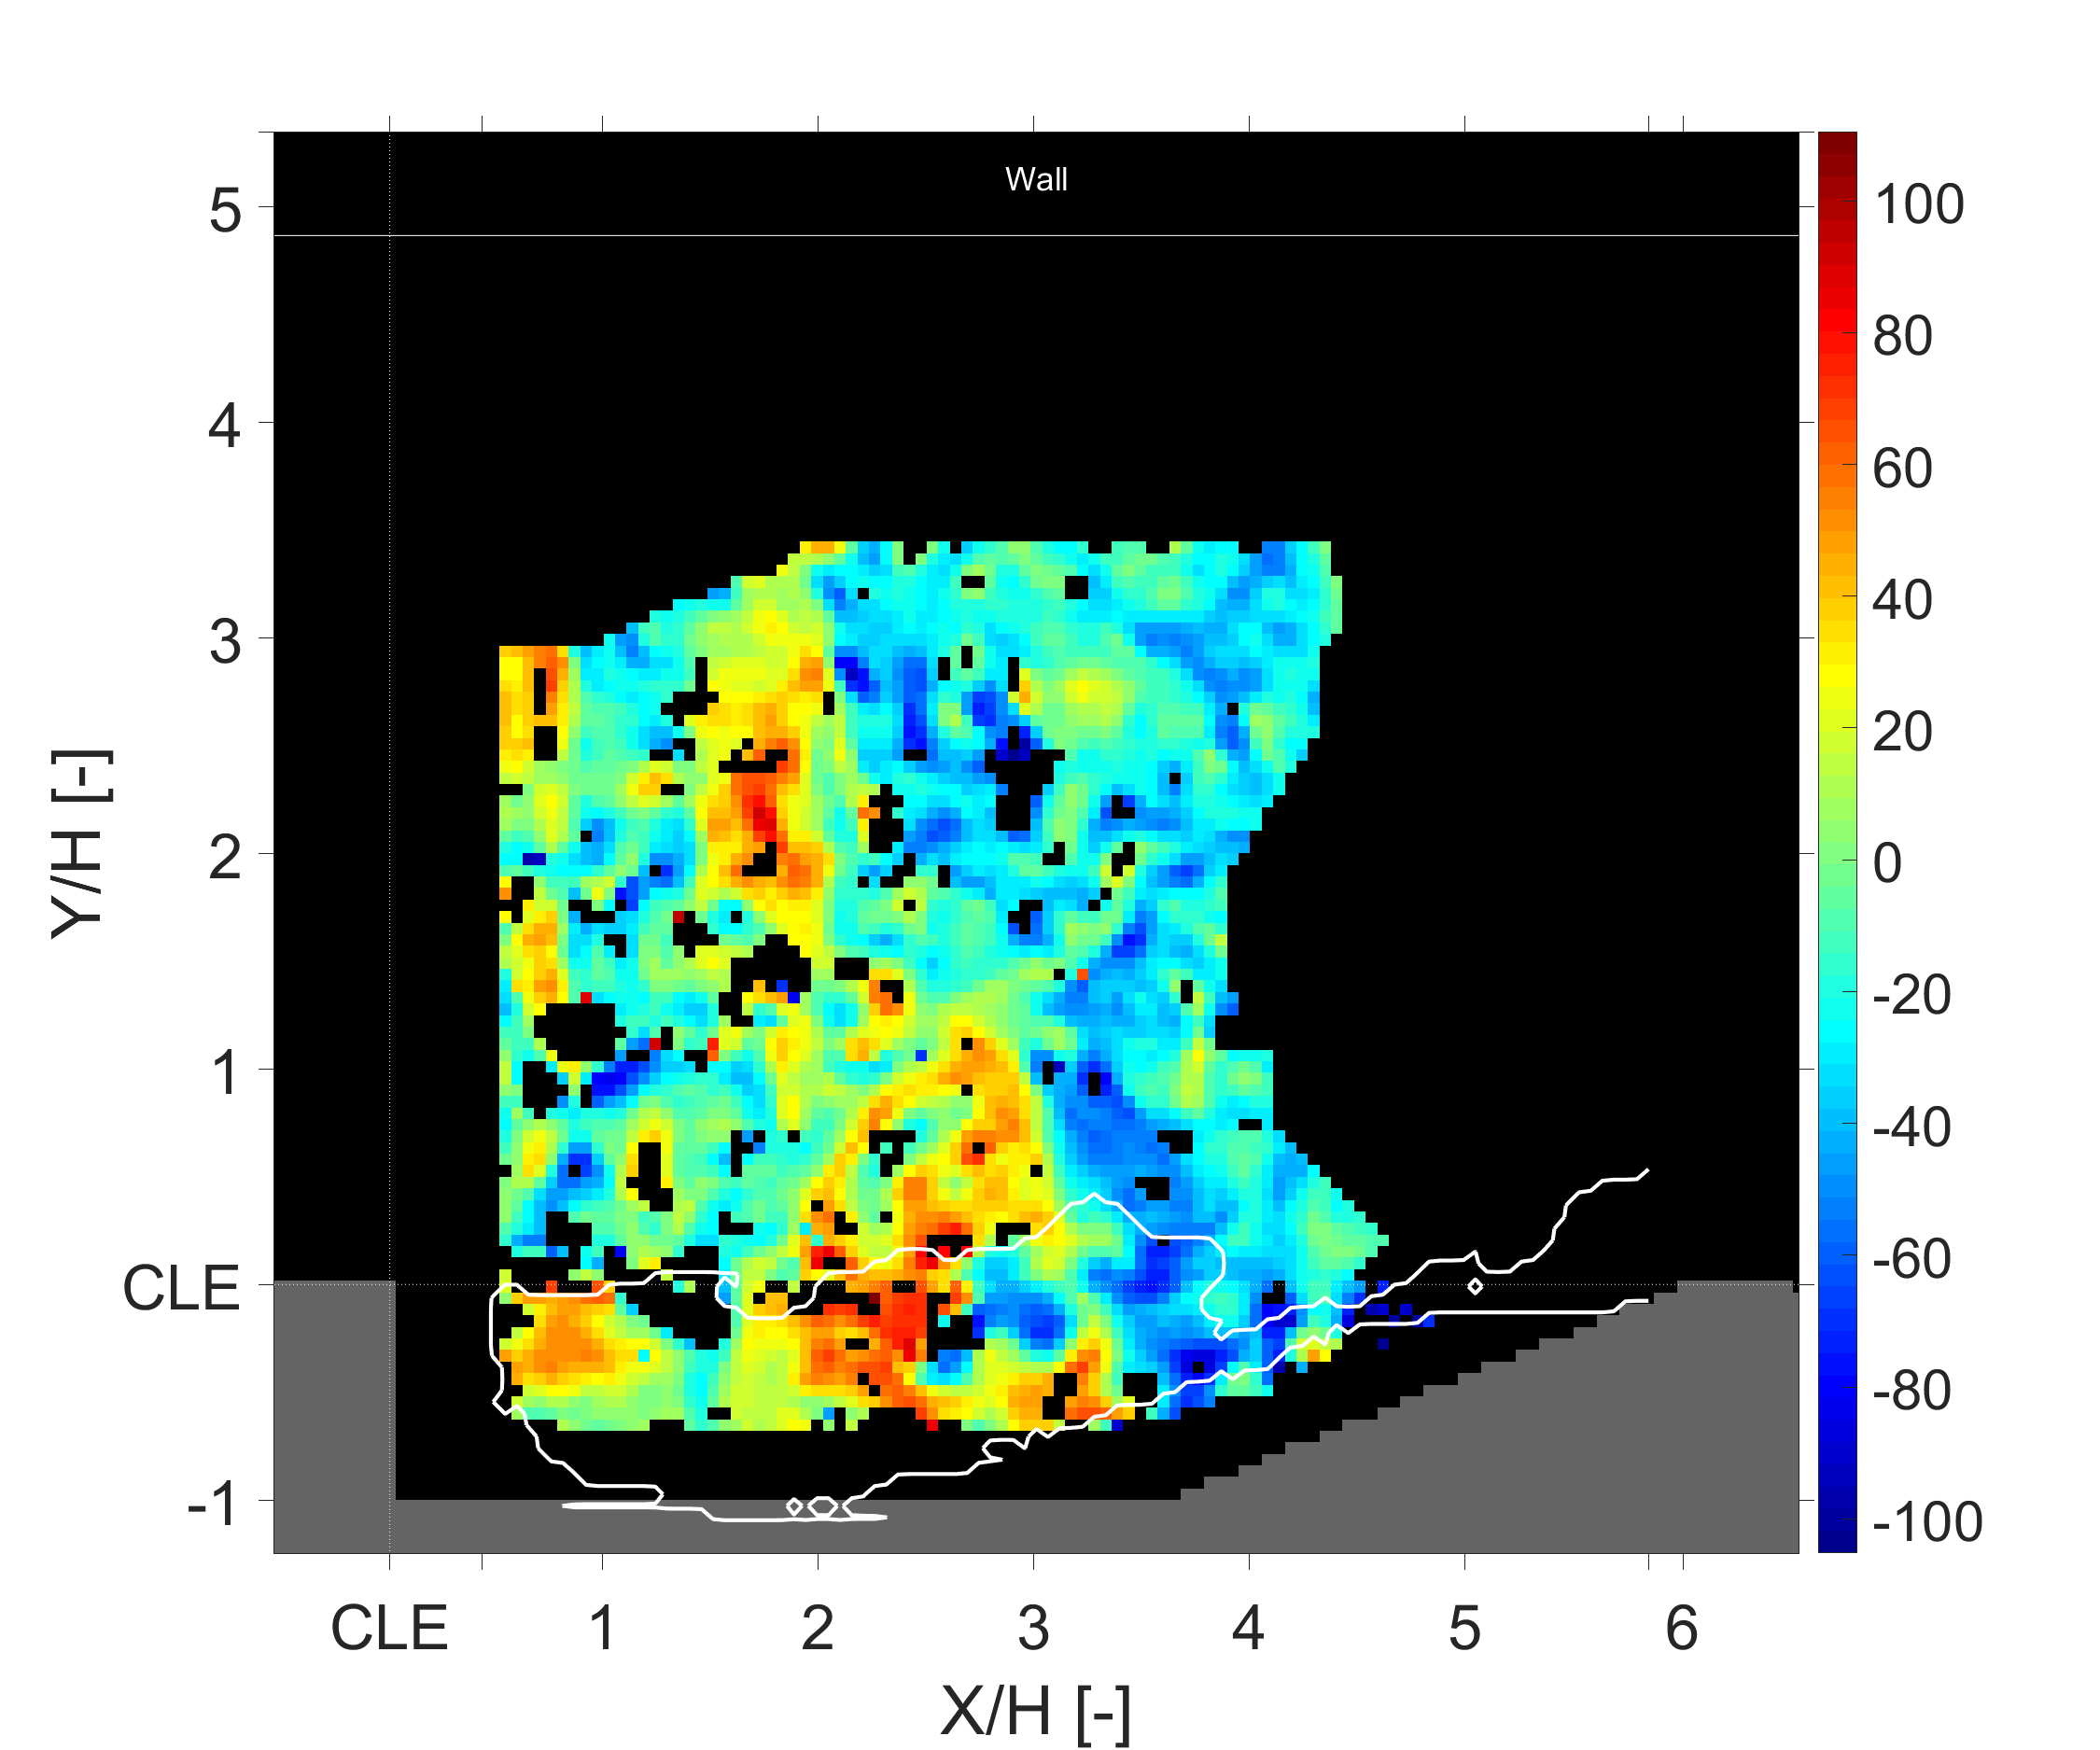
\includegraphics[height=2.5in, trim=0cm 0cm 0cm 0cm, clip]{figures/B1/combustion_instability/y/B1_Frame342_y}\hspace{0.5cm}}
% \subcaptionbox{State 4\label{fig:B1_Frame4y}}
%         {\hspace{0.5cm}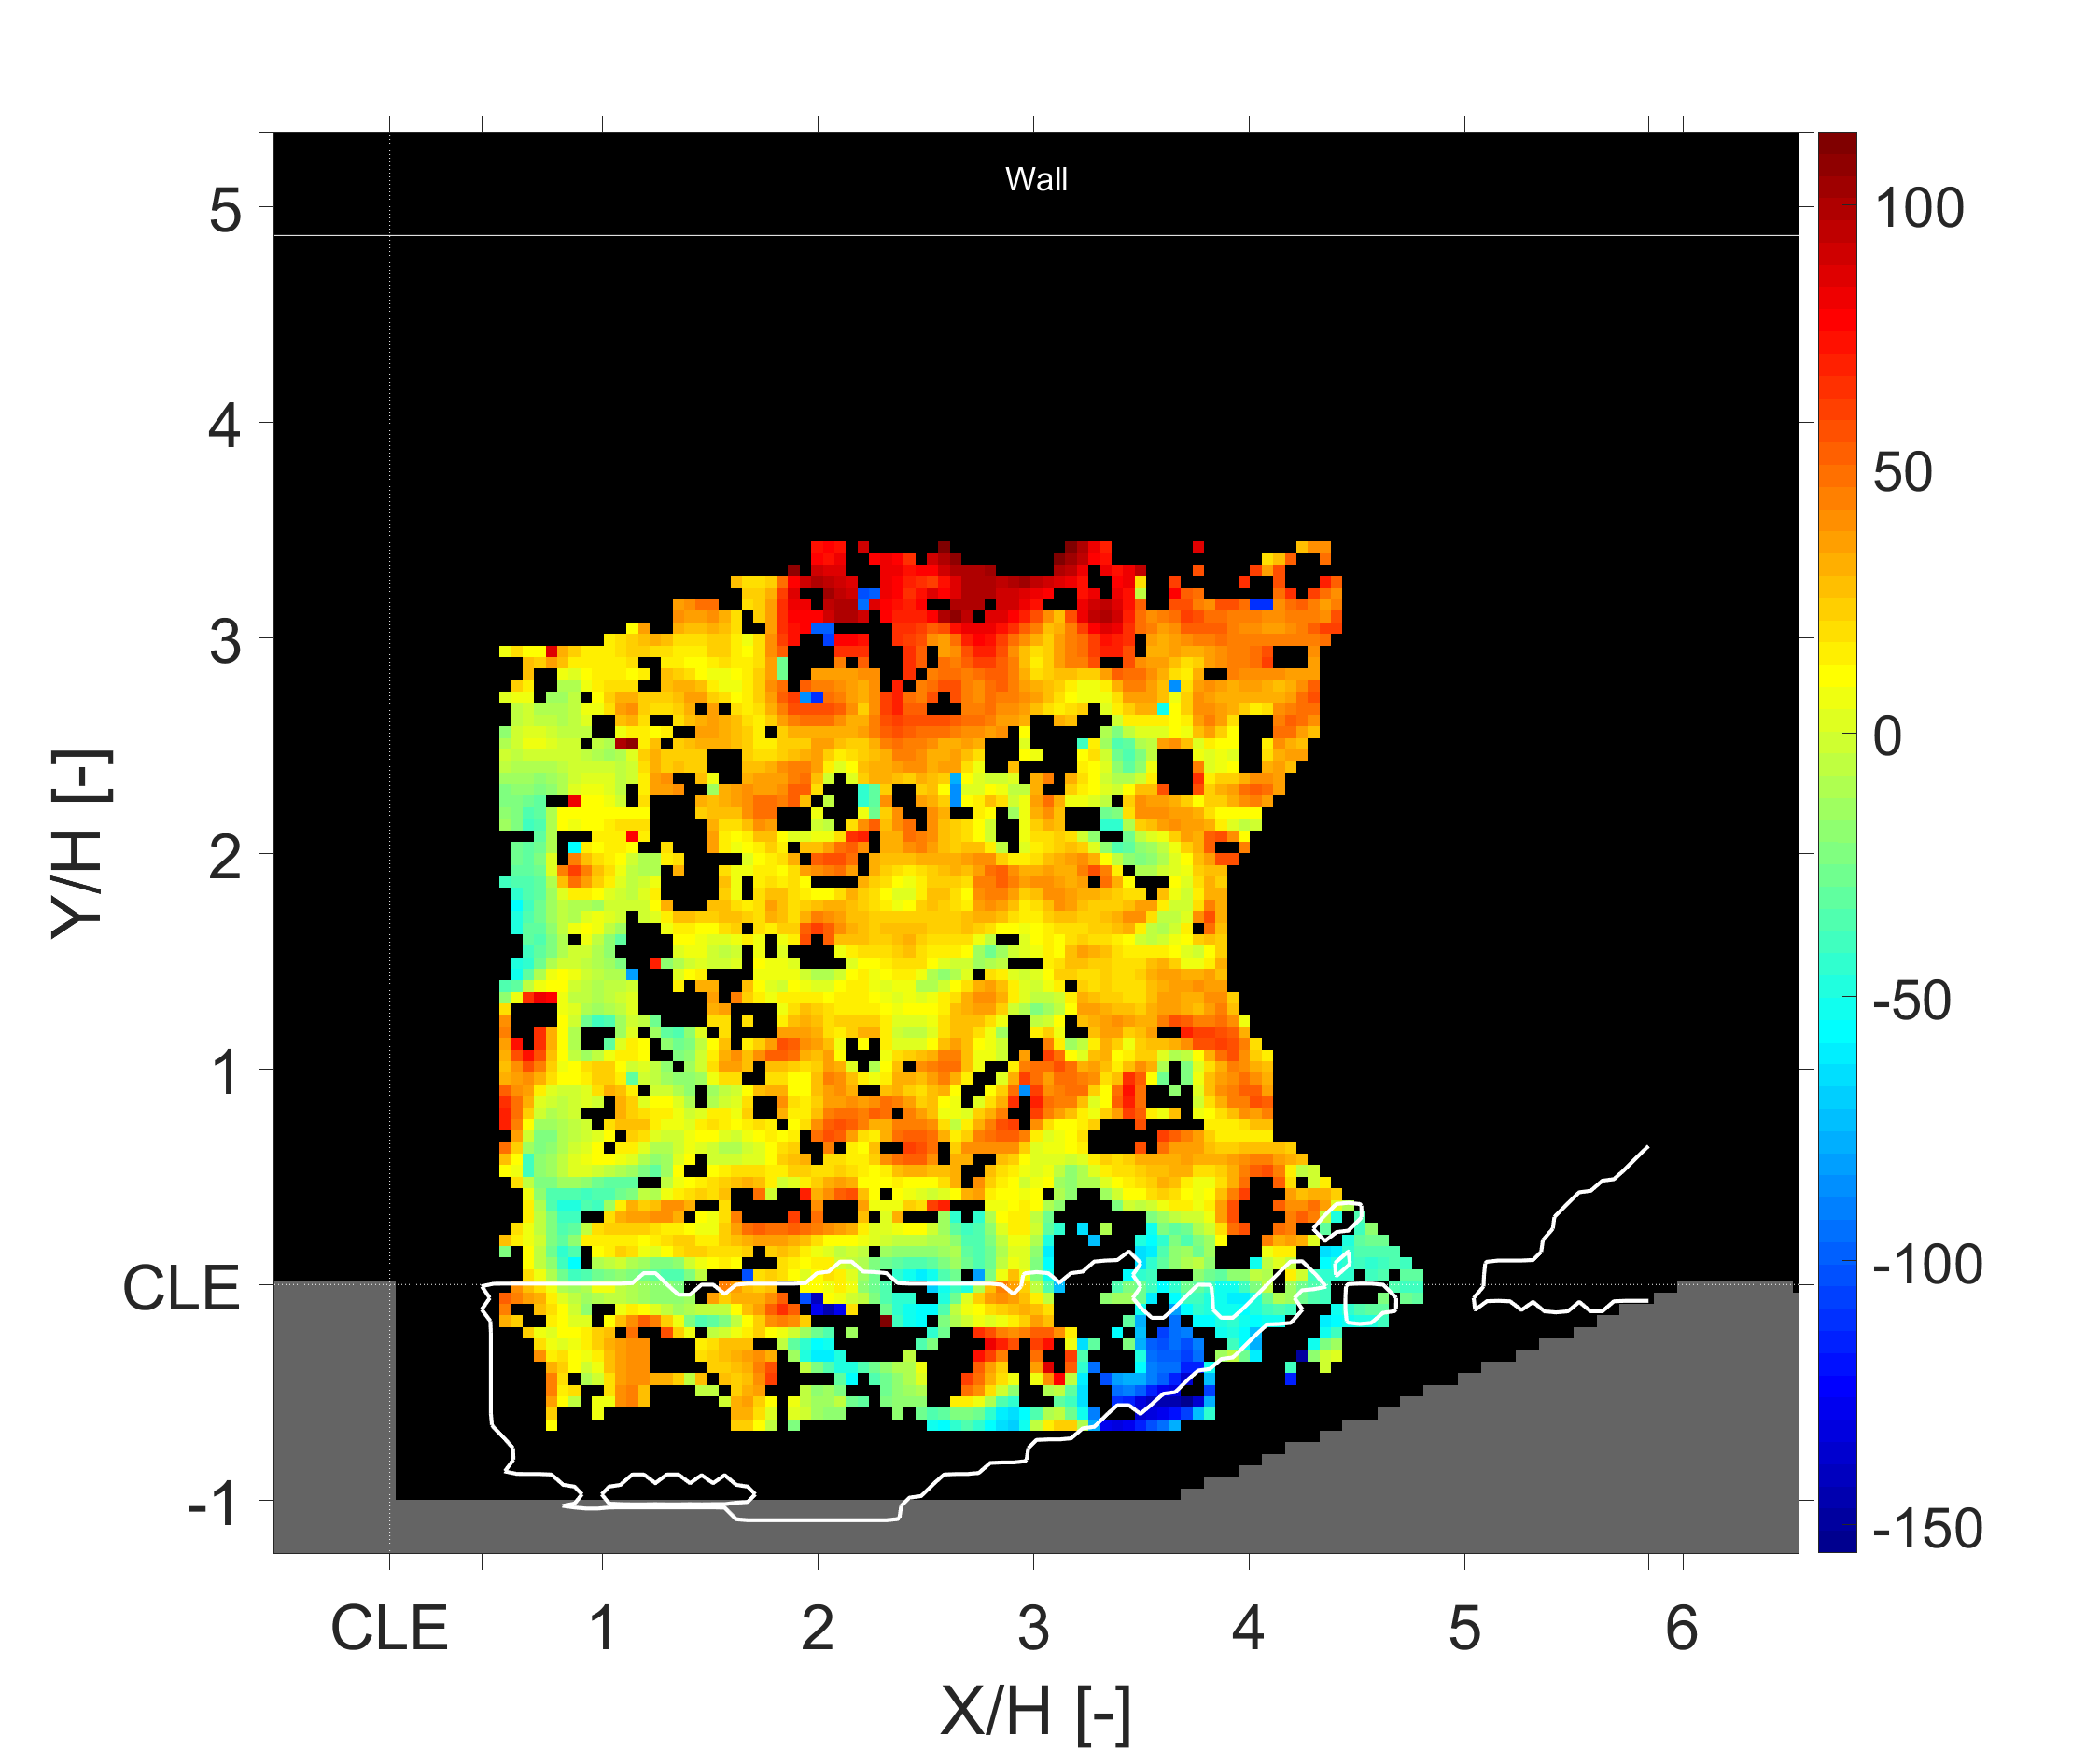
\includegraphics[height=2.5in, trim=0cm 0cm 0cm 0cm, clip]{figures/B1/combustion_instability/y/B1_Frame339_y}}
% \subcaptionbox{State 5\label{fig:B1_Frame5y}}
%         {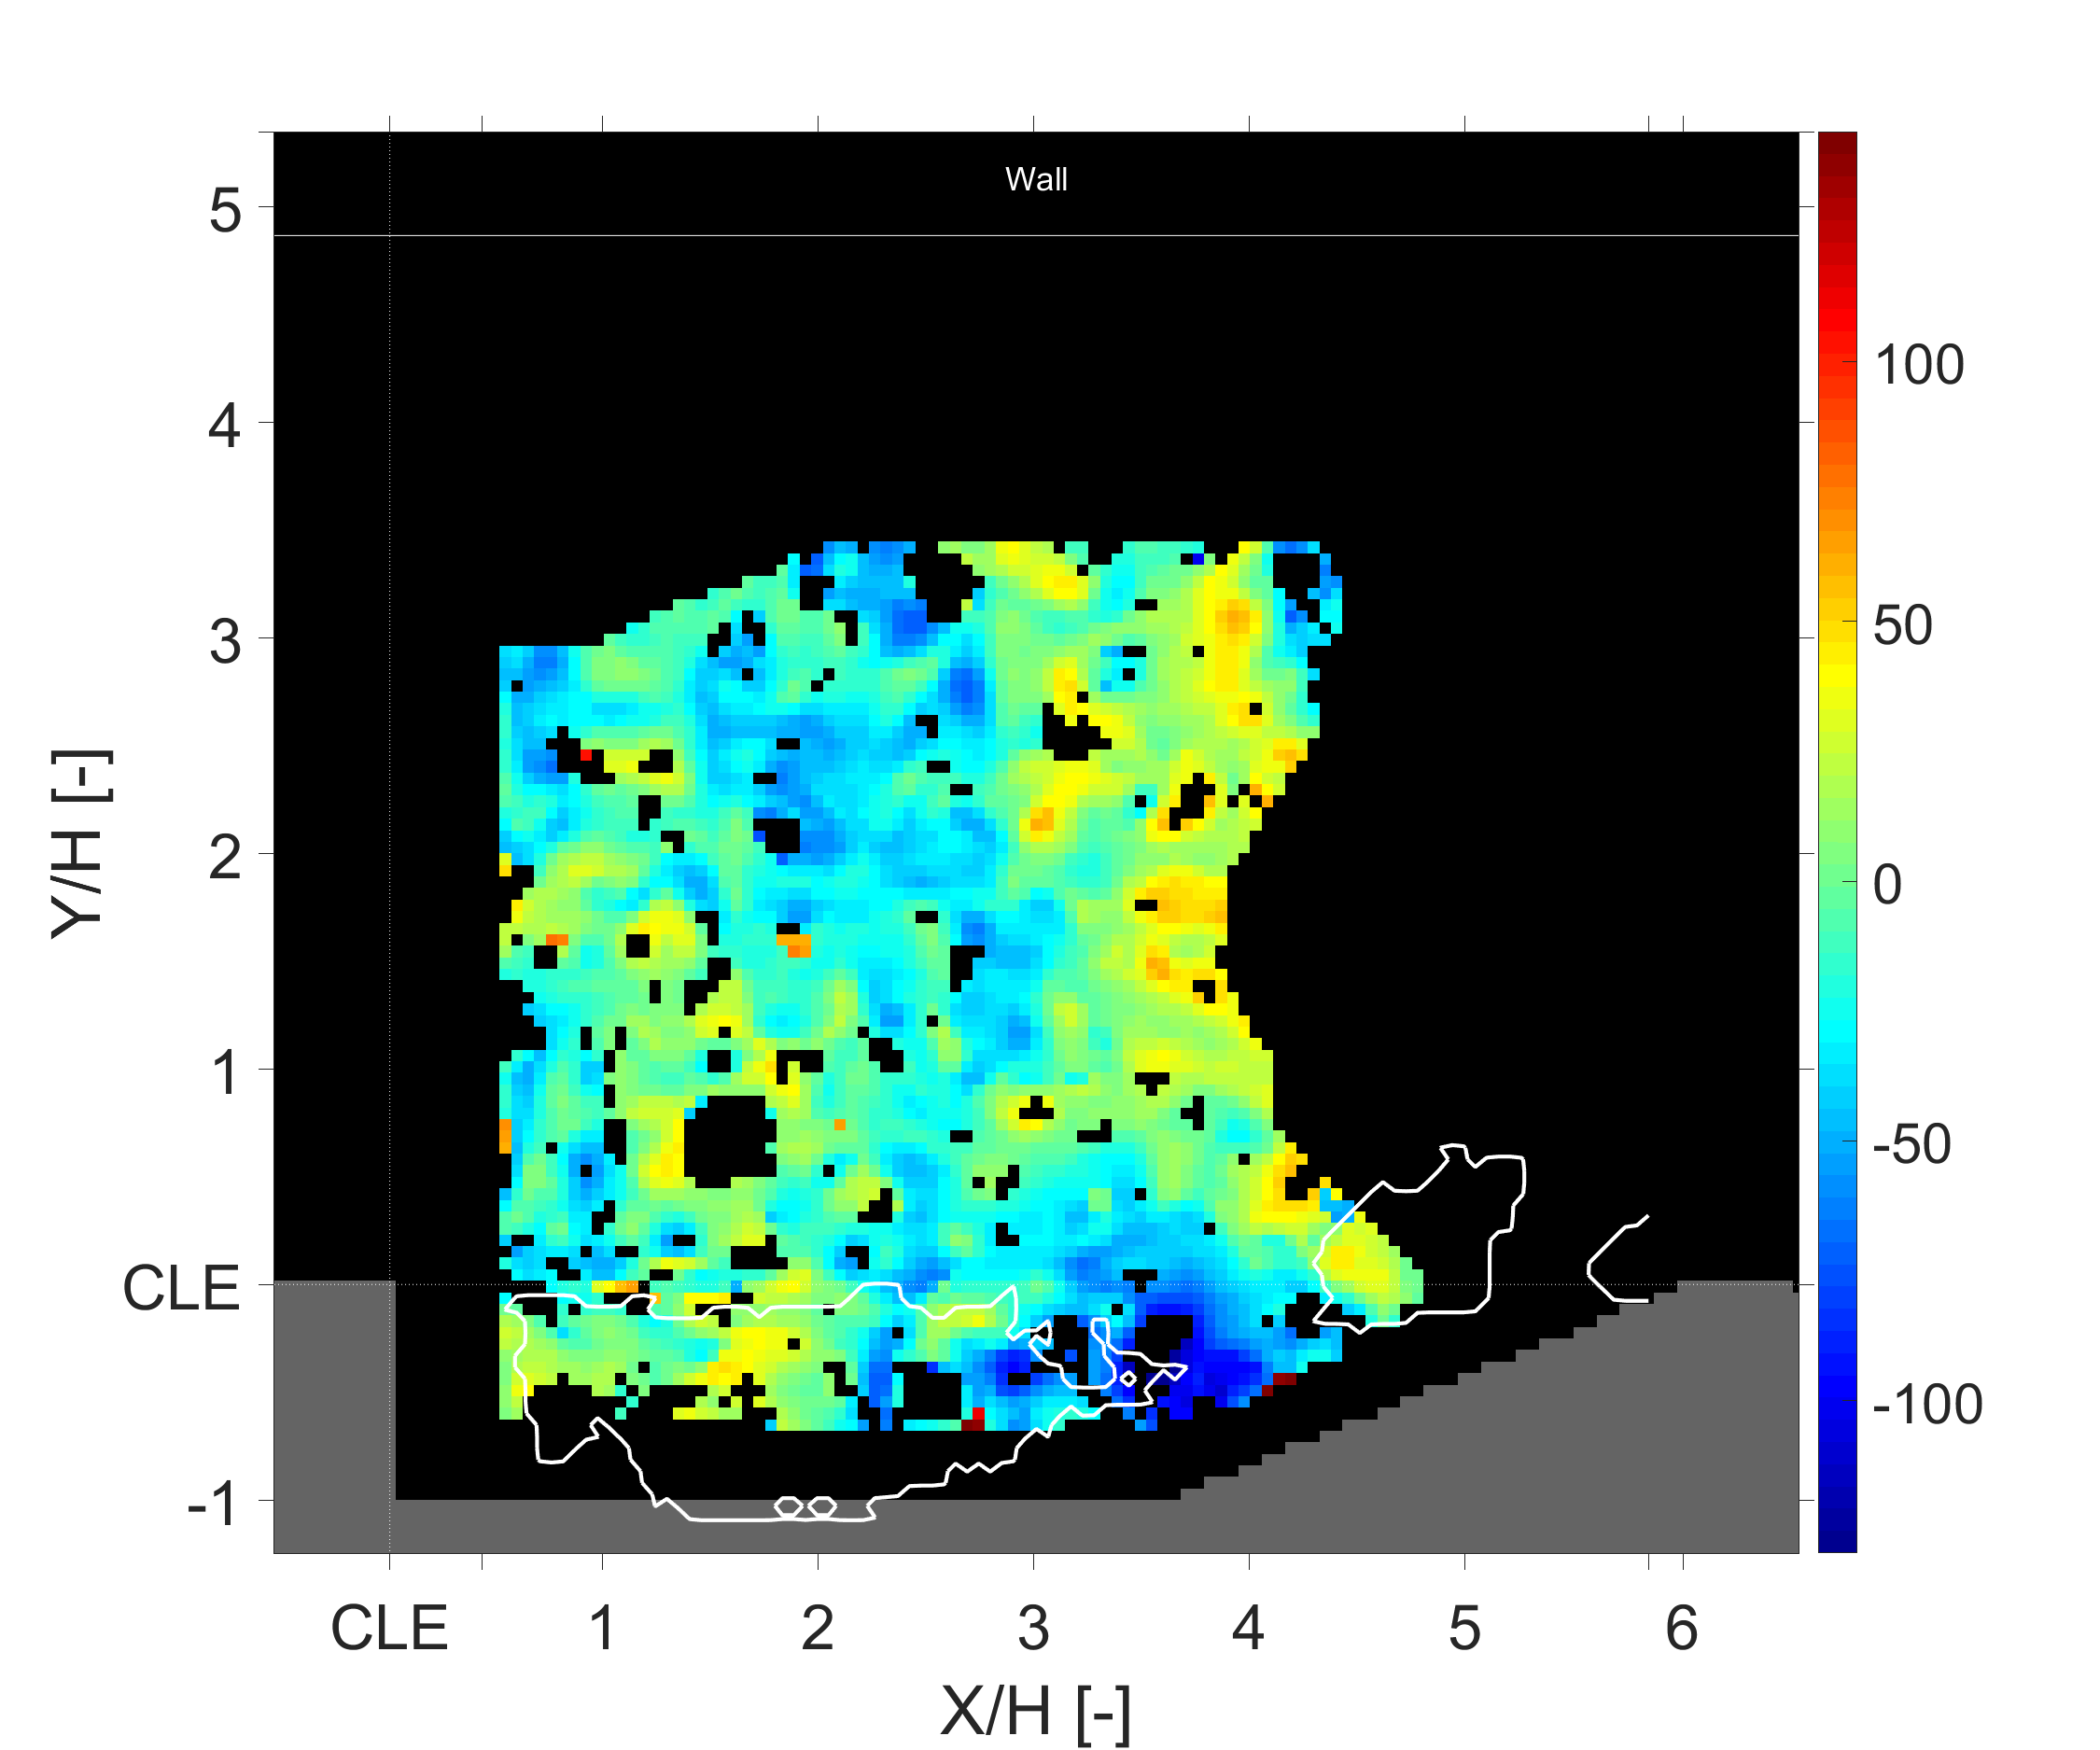
\includegraphics[height=2.5in, trim=0cm 0cm 0cm 0cm, clip]{figures/B1/combustion_instability/y/B1_Frame306_y.png}\hspace{0.5cm}}
%         \subcaptionbox{State 2 with duct velocities below average\label{fig:B1_Frame6y}}
%         {\hspace{0.5cm}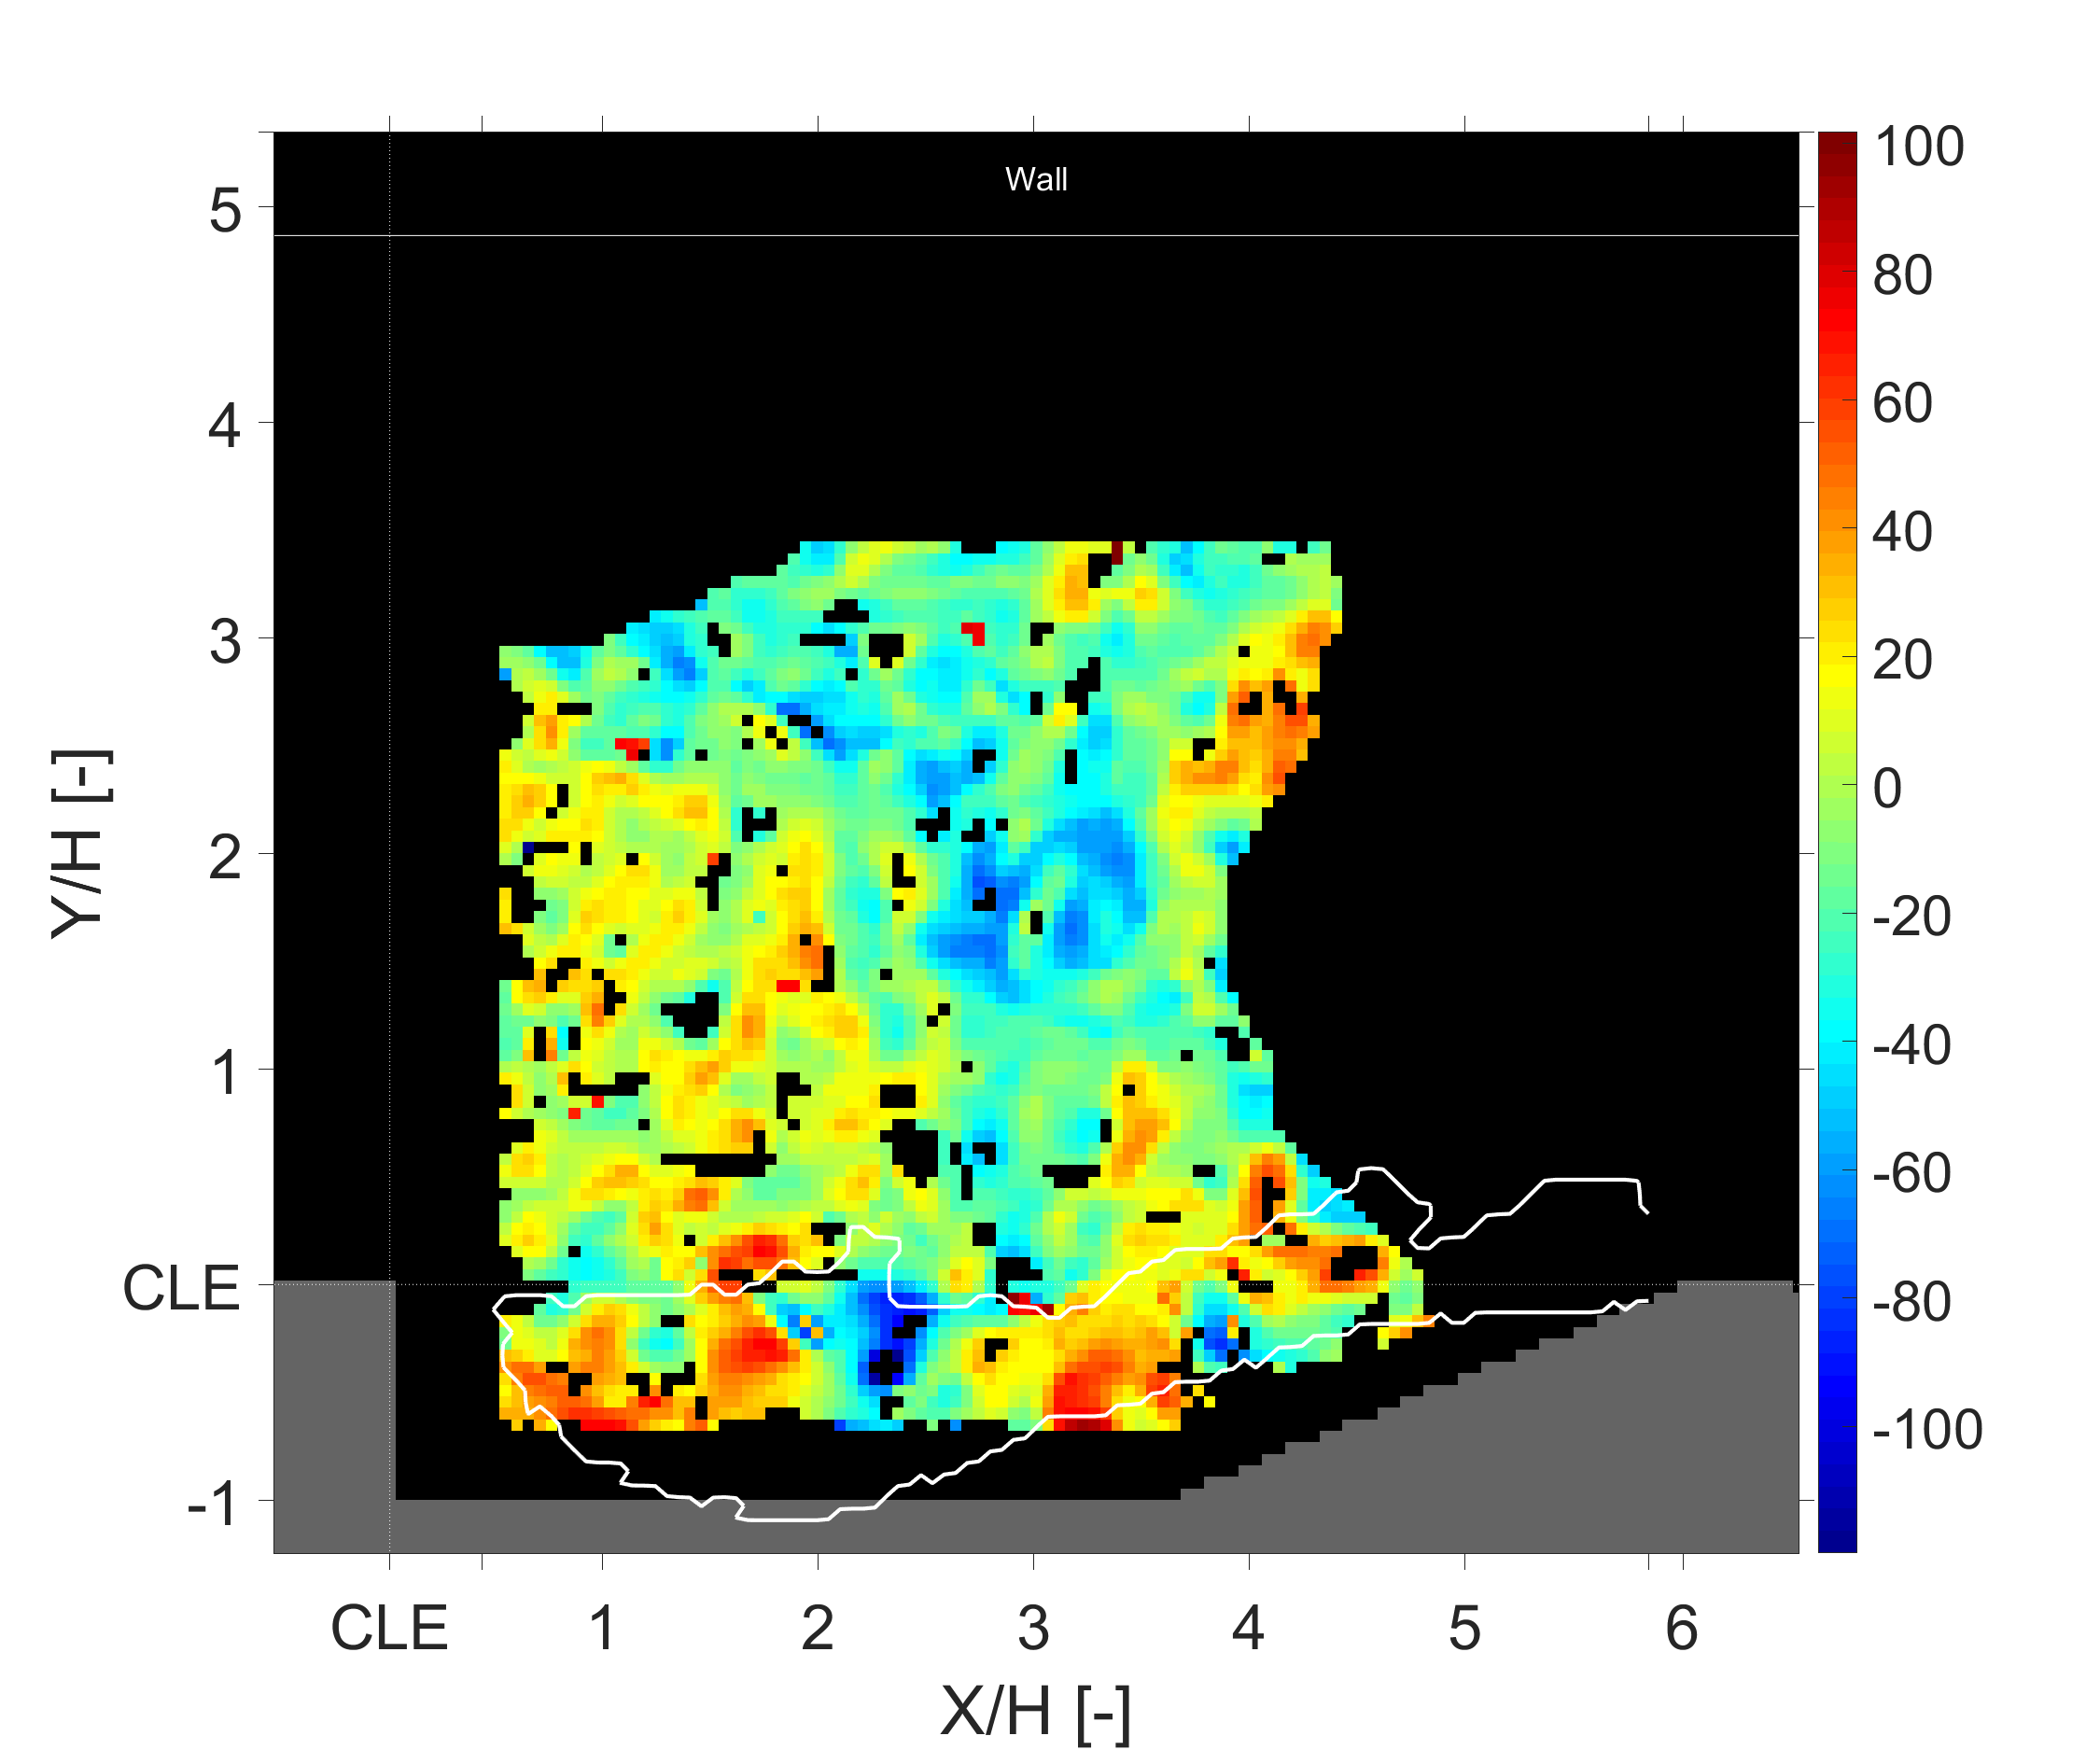
\includegraphics[height=2.5in, trim=0cm 0cm 0cm 0cm, clip]{figures/B1/combustion_instability/y/B1_Frame301_y}}
% \caption{$U_y$, select instantaneous PIV-PLIF frames.}\label{fig:ch3_inst_B1y}
% \end{figure}

\begin{figure}
\centering
\subcaptionbox{State 1\label{fig:B1_Frame1vec}}
      {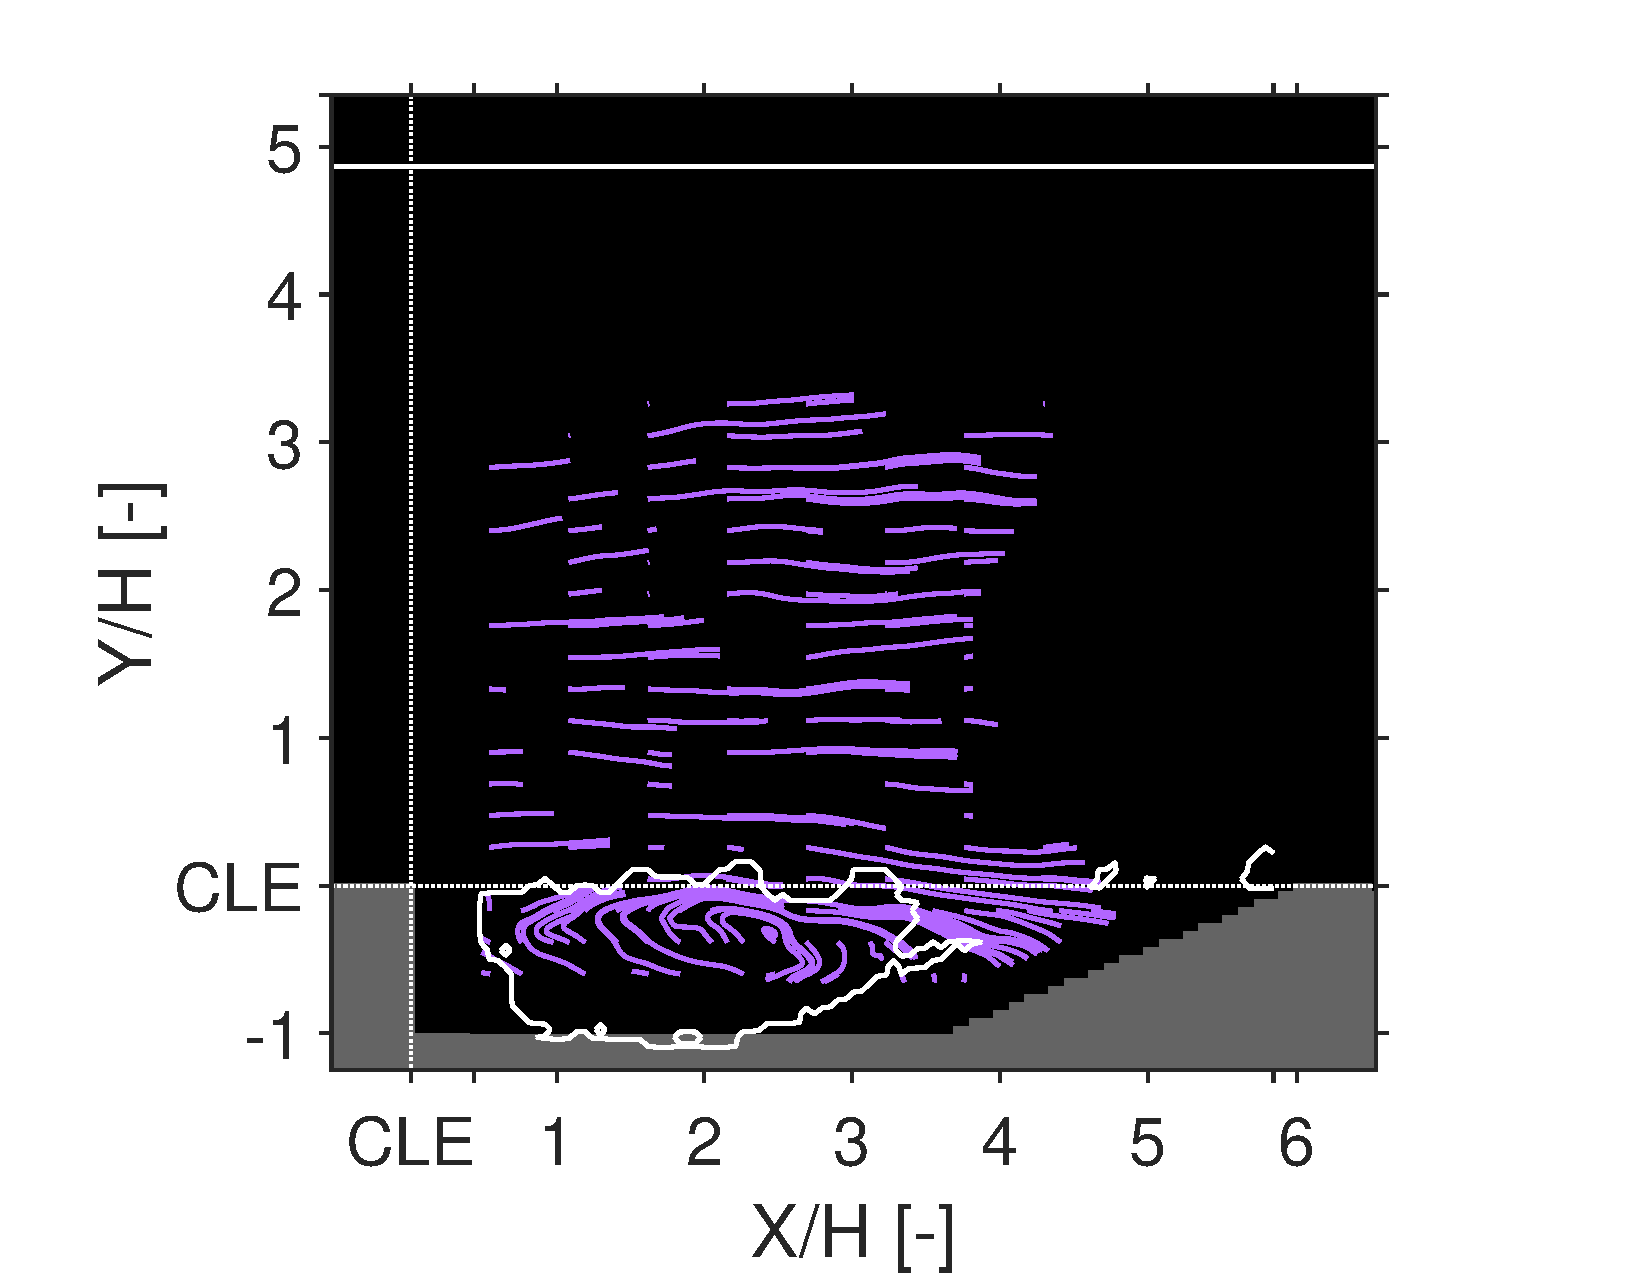
\includegraphics[width=3in,trim=0.35in 0 0.65in 0, clip]{figures/B1/combustion_instability/streamlines/B1_Frame331_v2.pdf}}
      \hspace{0.4cm}
\subcaptionbox{State 2\label{fig:B1_Frame2vec}}
                {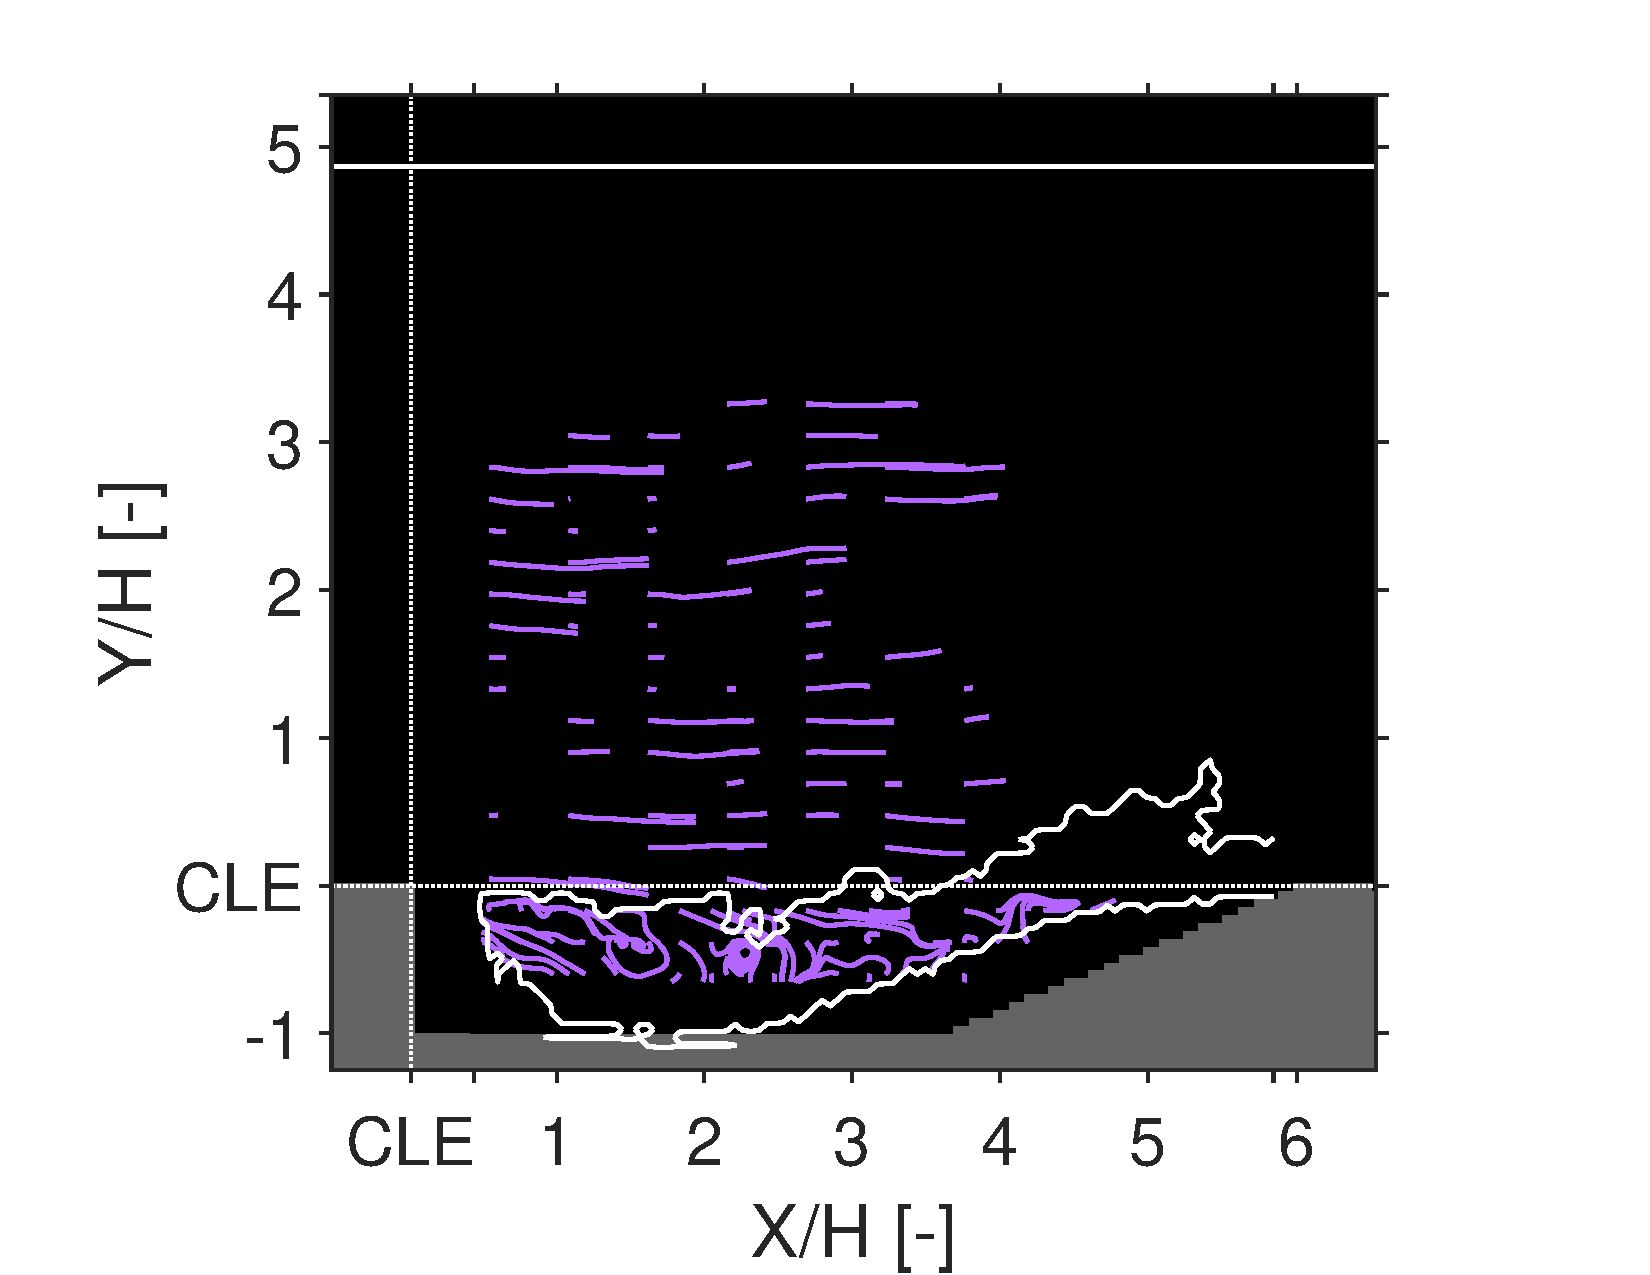
\includegraphics[width=3in,trim=0.35in 0 0.65in 0, clip]{figures/B1/combustion_instability/streamlines/B1_Frame329_v2.pdf}}
                \newline
\subcaptionbox{State 2'\label{fig:B1_Frame3vec}}
        {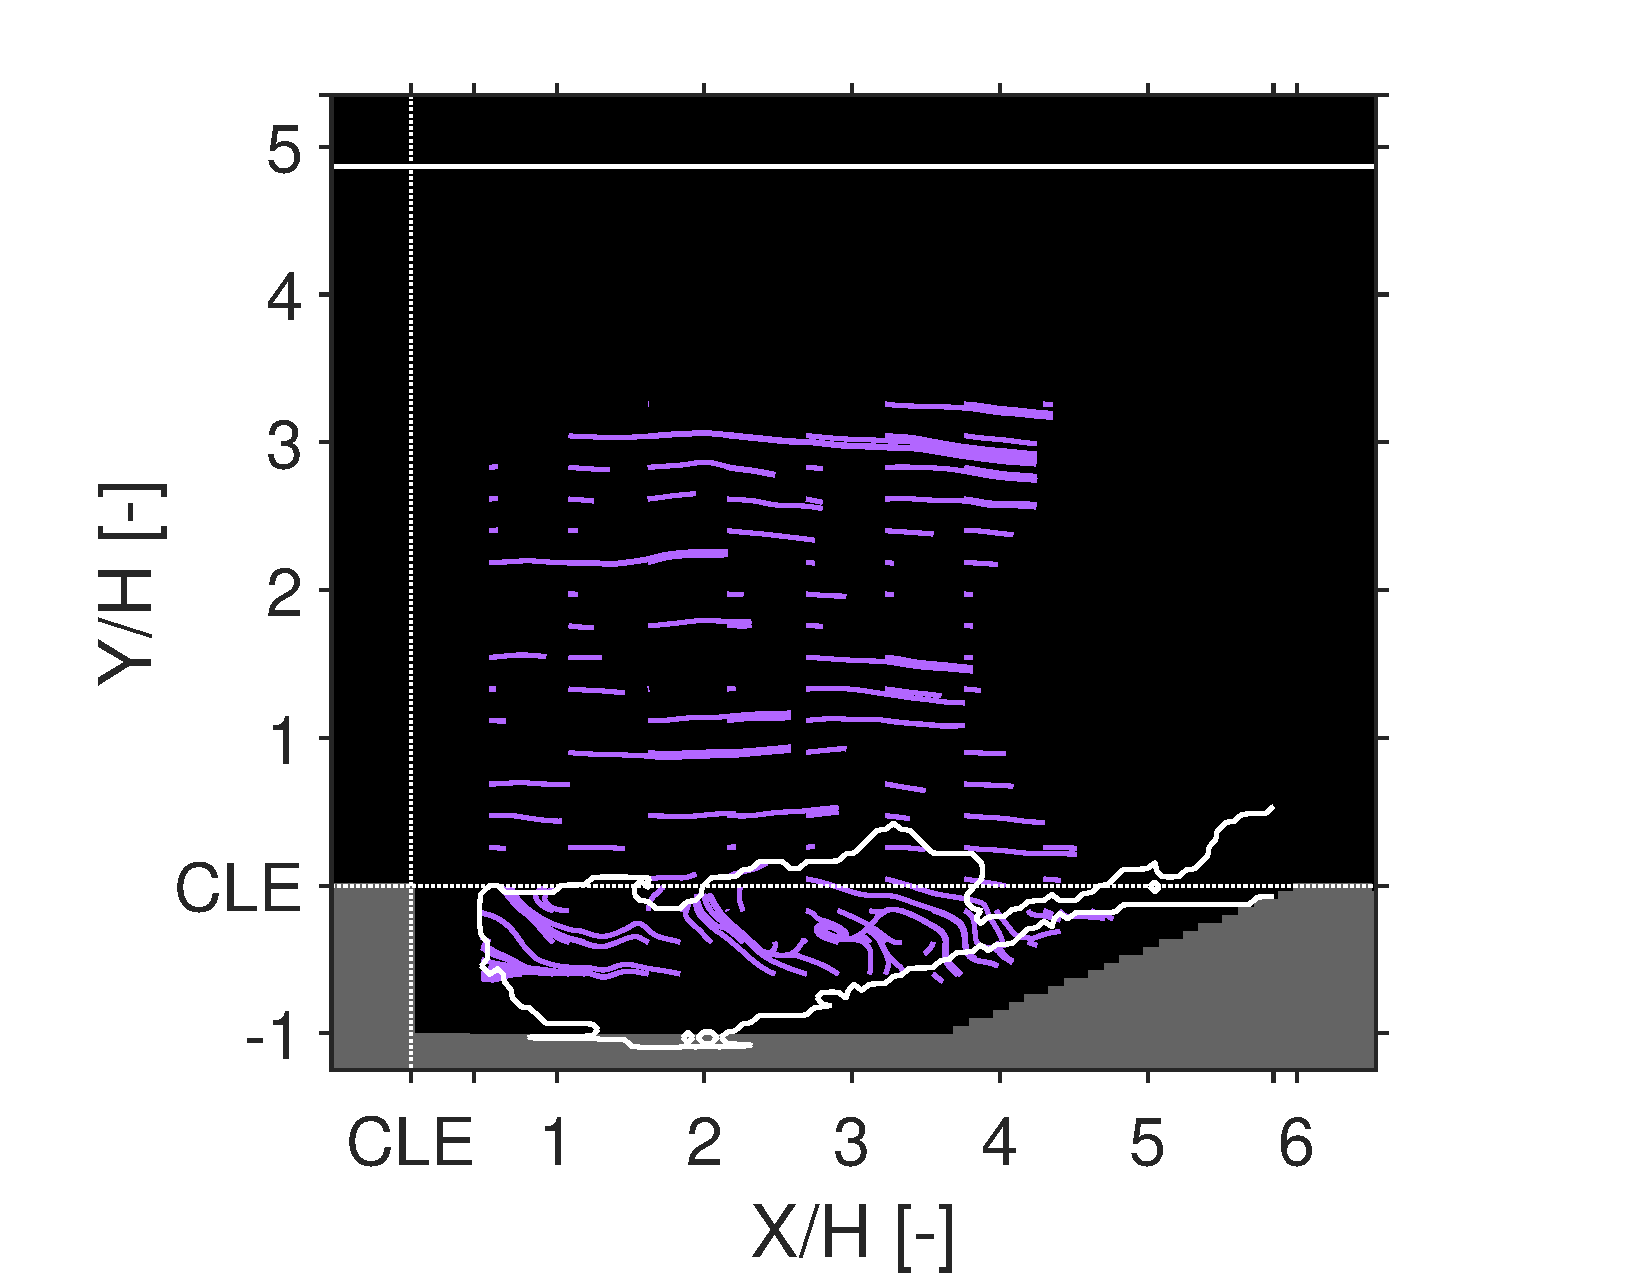
\includegraphics[width=3in,trim=0.35in 0 0.65in 0, clip]{figures/B1/combustion_instability/streamlines/B1_Frame342_v2.pdf}}
        \hspace{0.4cm}
\subcaptionbox{State 3\label{fig:B1_Frame4vec}}
                {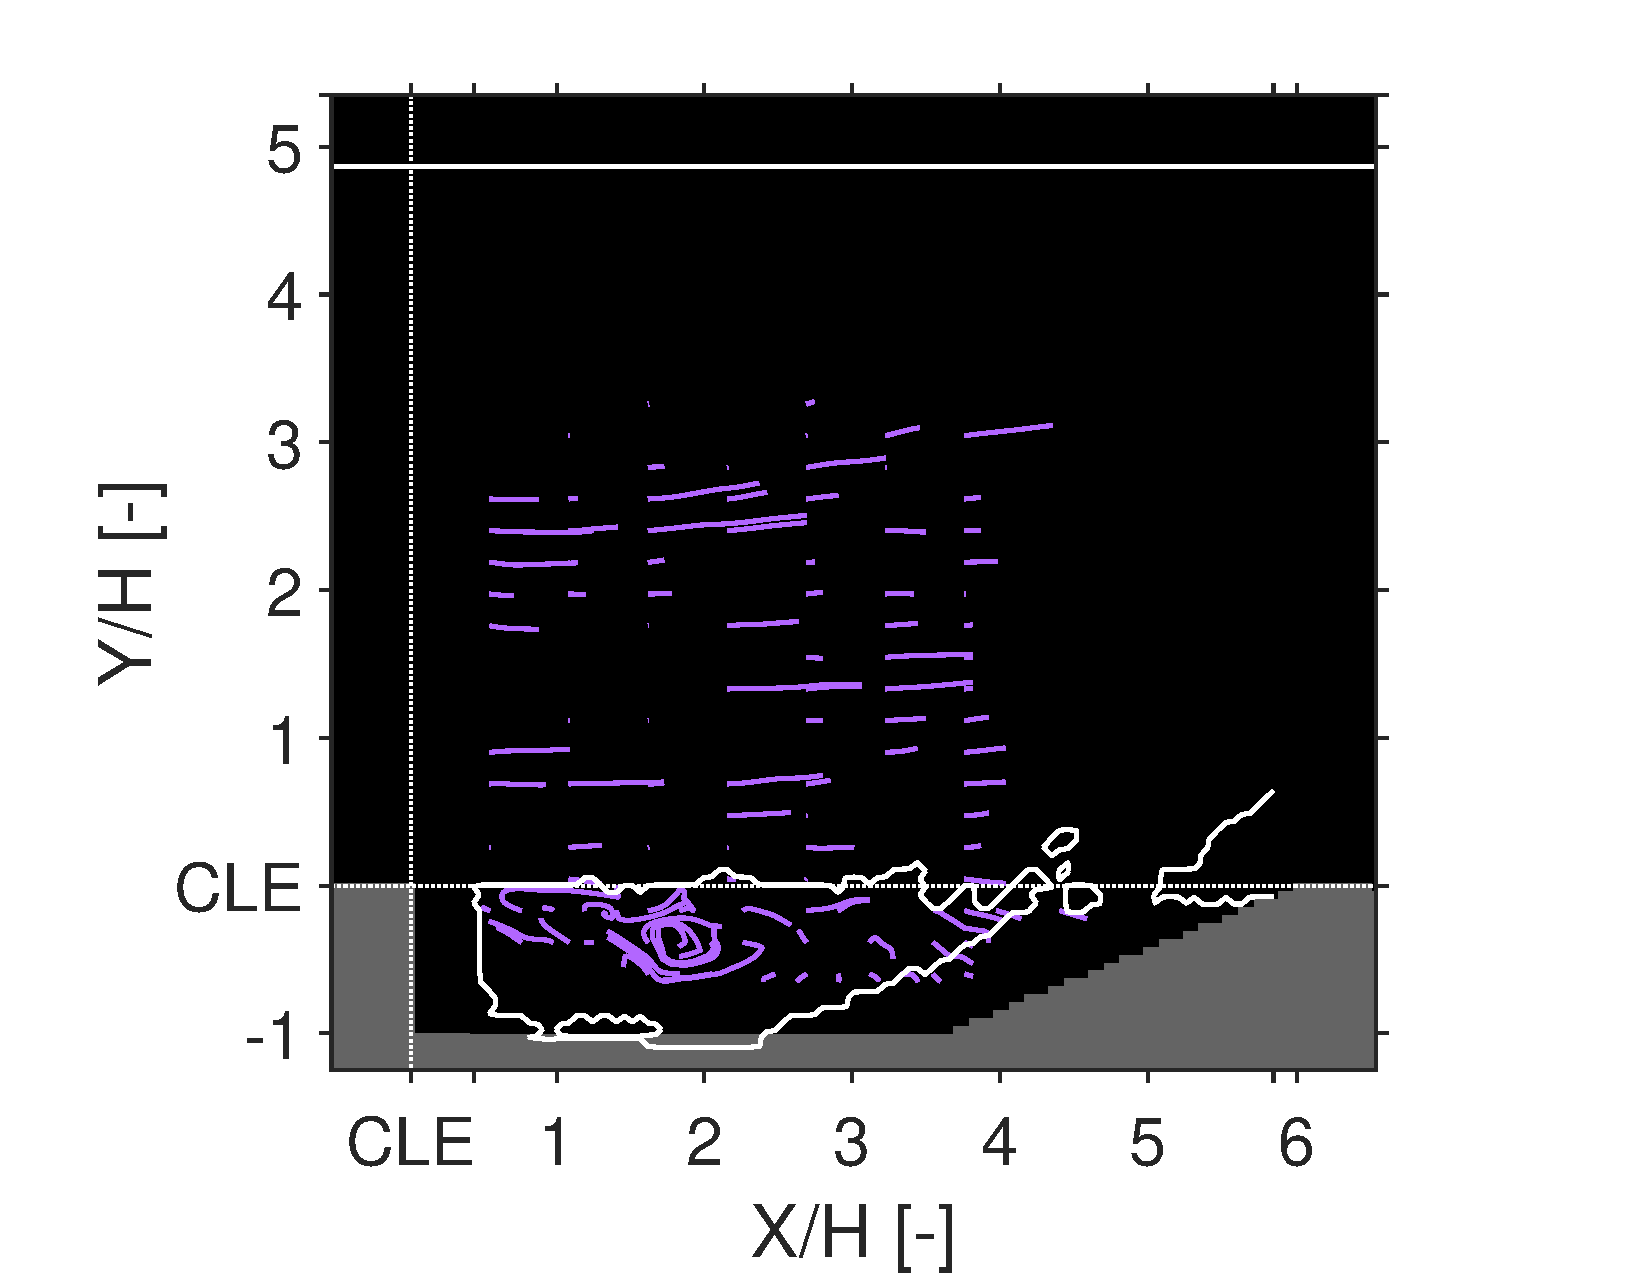
\includegraphics[width=3in,trim=0.35in 0 0.65in 0, clip]{figures/B1/combustion_instability/streamlines/B1_Frame339_v2.pdf}}
                \newline
 \subcaptionbox{State 3'\label{fig:B1_Frame5vec}}
         {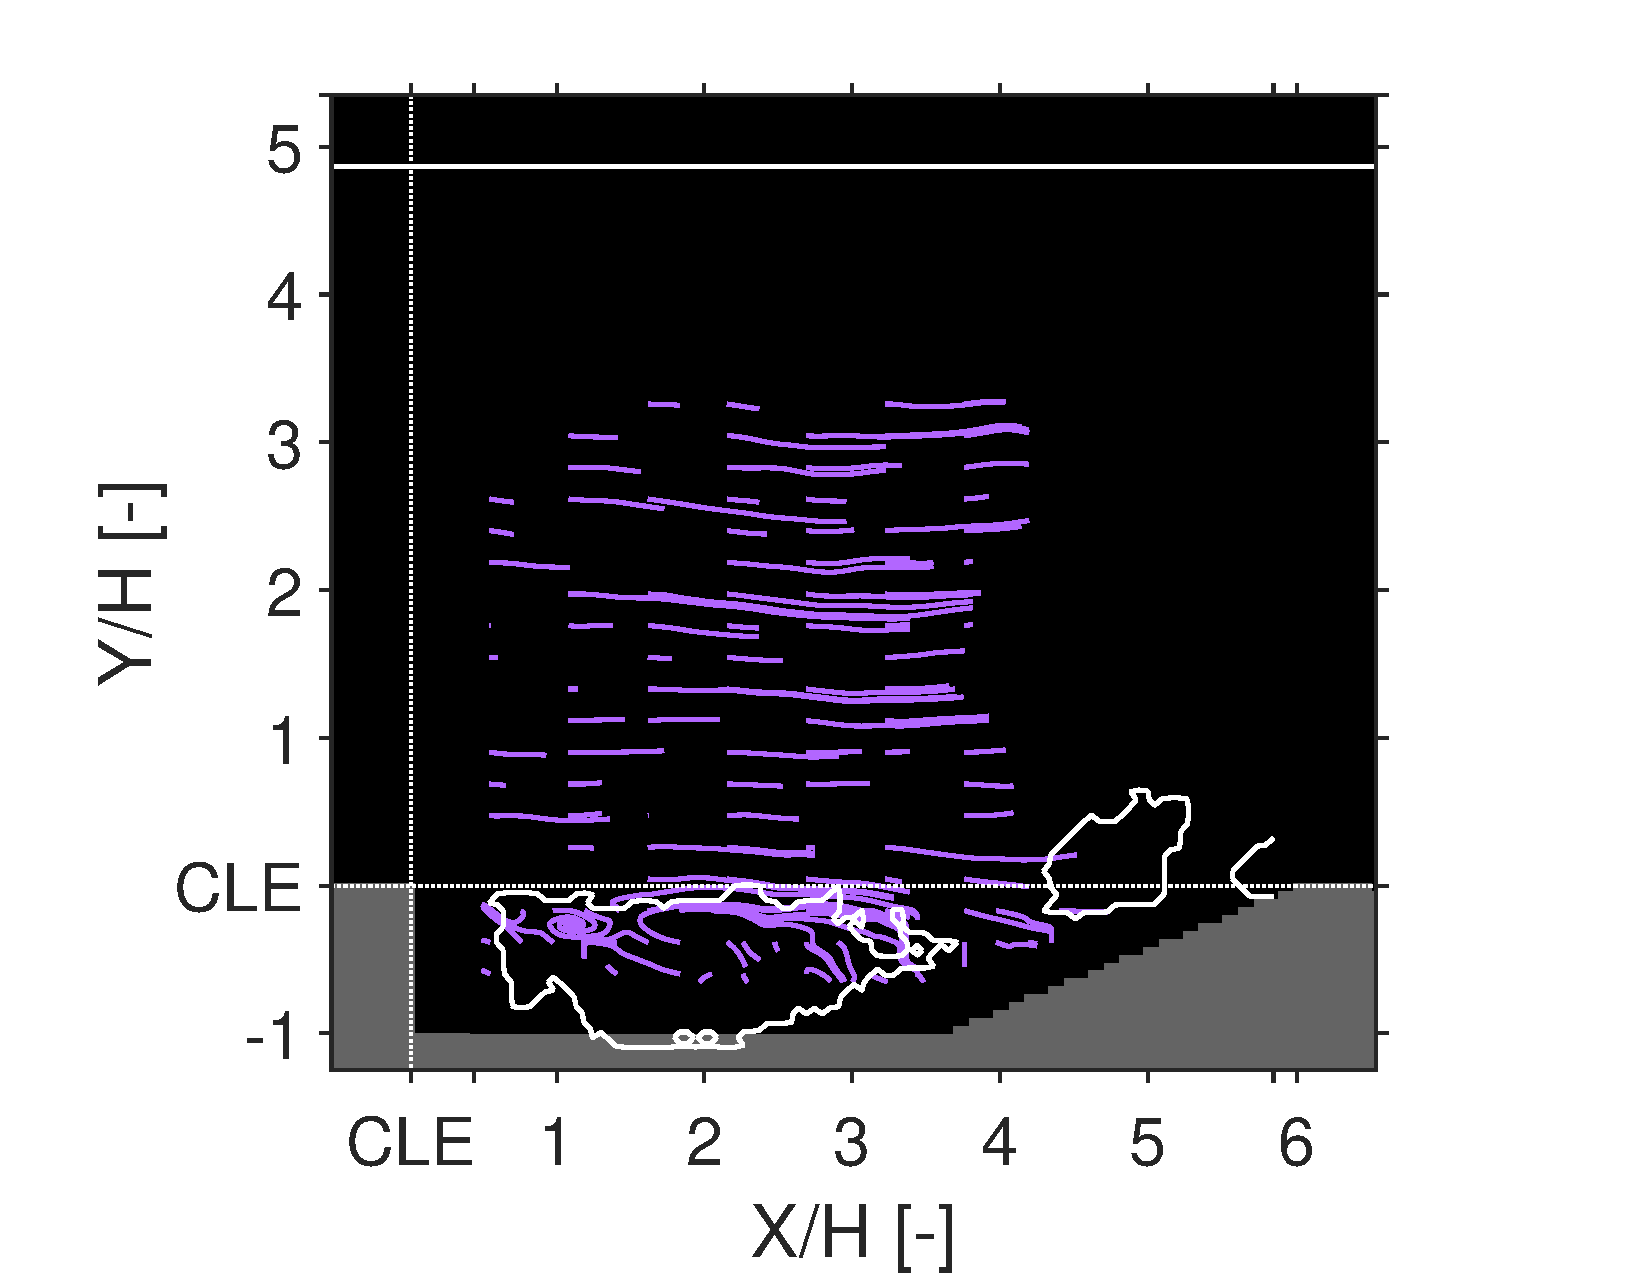
\includegraphics[width=3in,trim=0.35in 0 0.65in 0, clip]{figures/B1/combustion_instability/streamlines/B1_Frame306_v2.pdf}}
         \hspace{0.4cm}
        \subcaptionbox{State 2 with duct velocities below average\label{fig:B1_Frame6vec}}
                {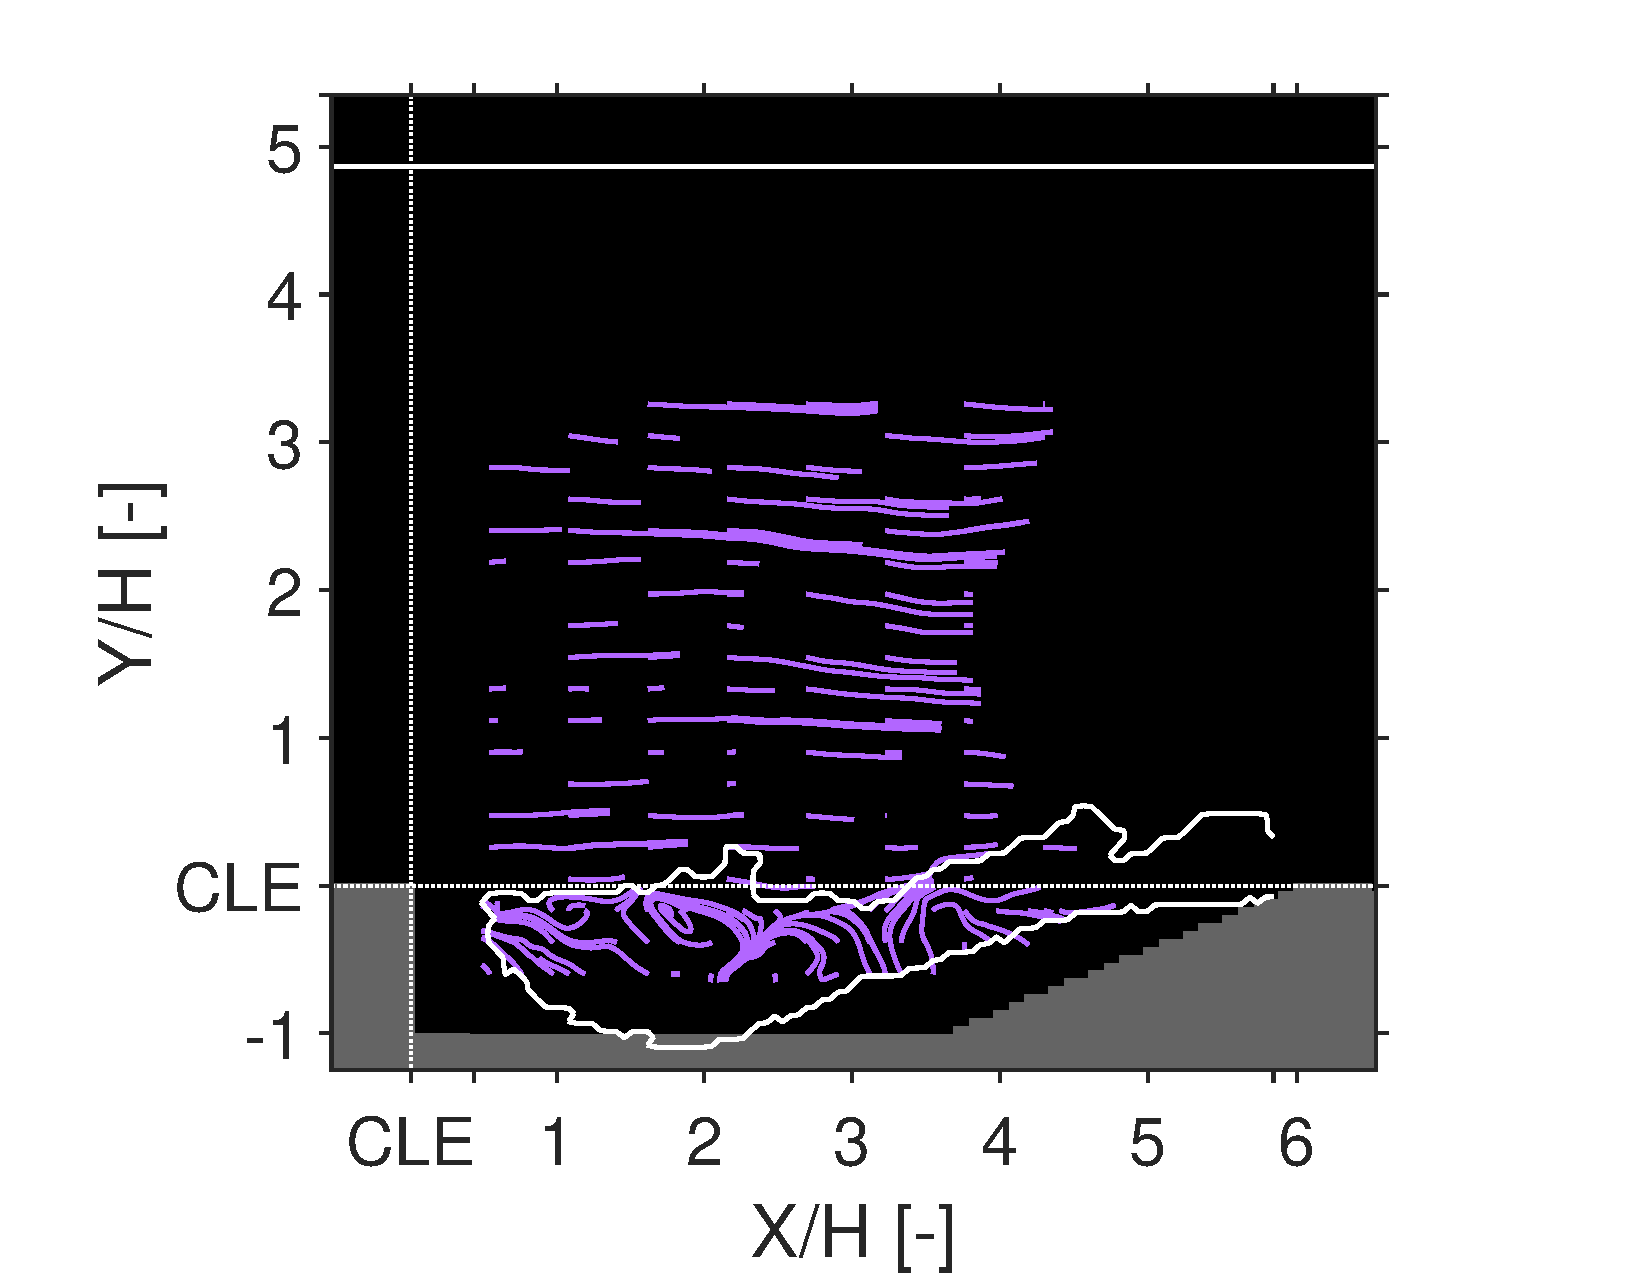
\includegraphics[width=3in,trim=0.35in 0 0.65in 0, clip]{figures/B1/combustion_instability/streamlines/B1_Frame301_v2.pdf}}
\caption{Streamlines, select instantaneous PIV-PLIF frames.}\label{fig:ch3_inst_B1vec}
\end{figure}

For all three states, the cavity flame closely abides by the shear layer, wrinkles around the shear-layer eddies (identified by high swirling strength values in Fig. \ref{fig:ch3_inst_ST}), and is either continuous or split into two regions. The shear-layer eddies serve to exchange combustion radicals generated in the cavity with the fresh premixed flow from the duct. These eddies are of similar size to eddies found in the free stream (Fig. \ref{fig:ch3_inst_ST}). In addition, large scale free stream fluctuations are observed in the streamlines and vectors of Figs. \ref{fig:ch3_inst_B1} and \ref{fig:ch3_inst_ST}. Measurements with the shear layer impinging on the cavity ramp are correlated with a negative transverse velocity in the free stream flow close to the cavity. The above observations suggest that spatial scales on the order of $H$ in the cavity flame are coupled with the free stream scales.

\begin{figure}
\centering
\subcaptionbox{State 1\label{fig:B1_R1_ST}}
        {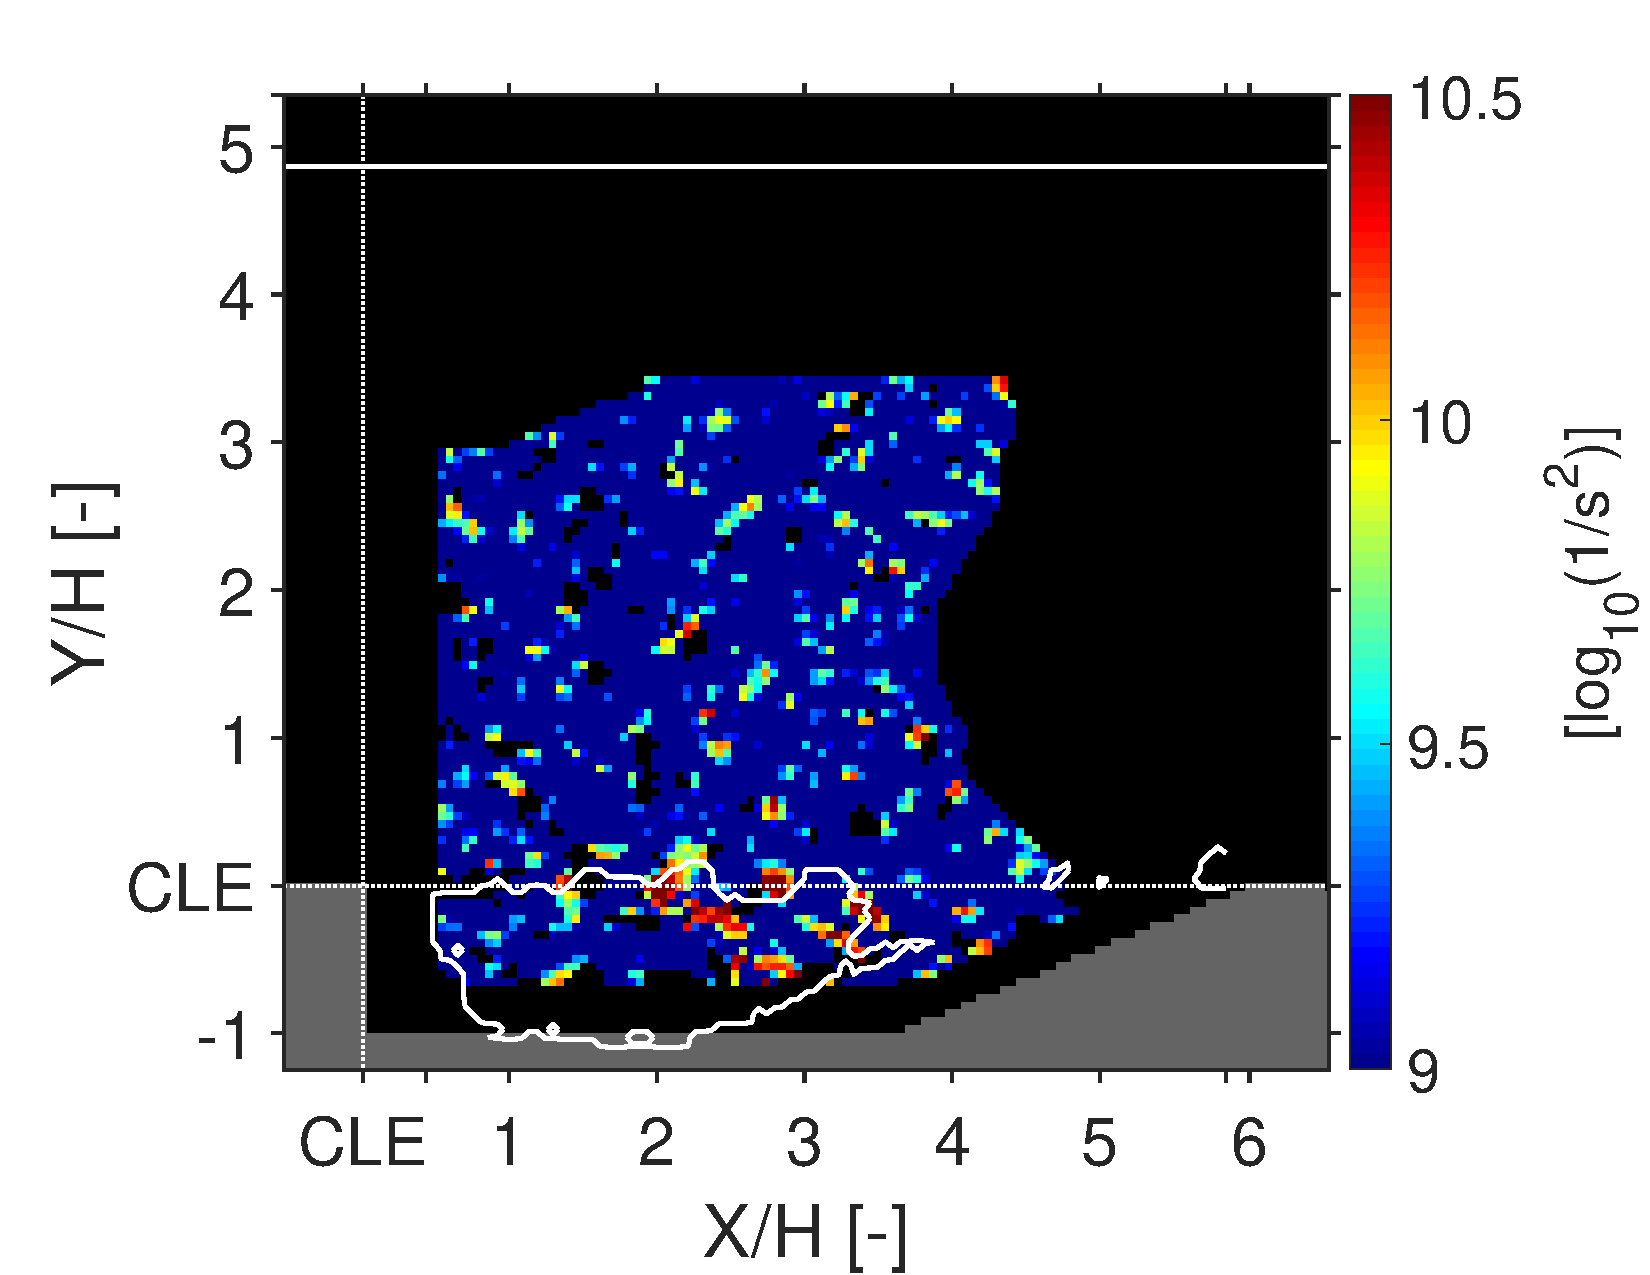
\includegraphics[width=3.25in]{figures/B1/B1_swirling_strength/B1_Frame331.pdf}} \\
\subcaptionbox{State 2\label{fig:B1_R2_ST}}{
        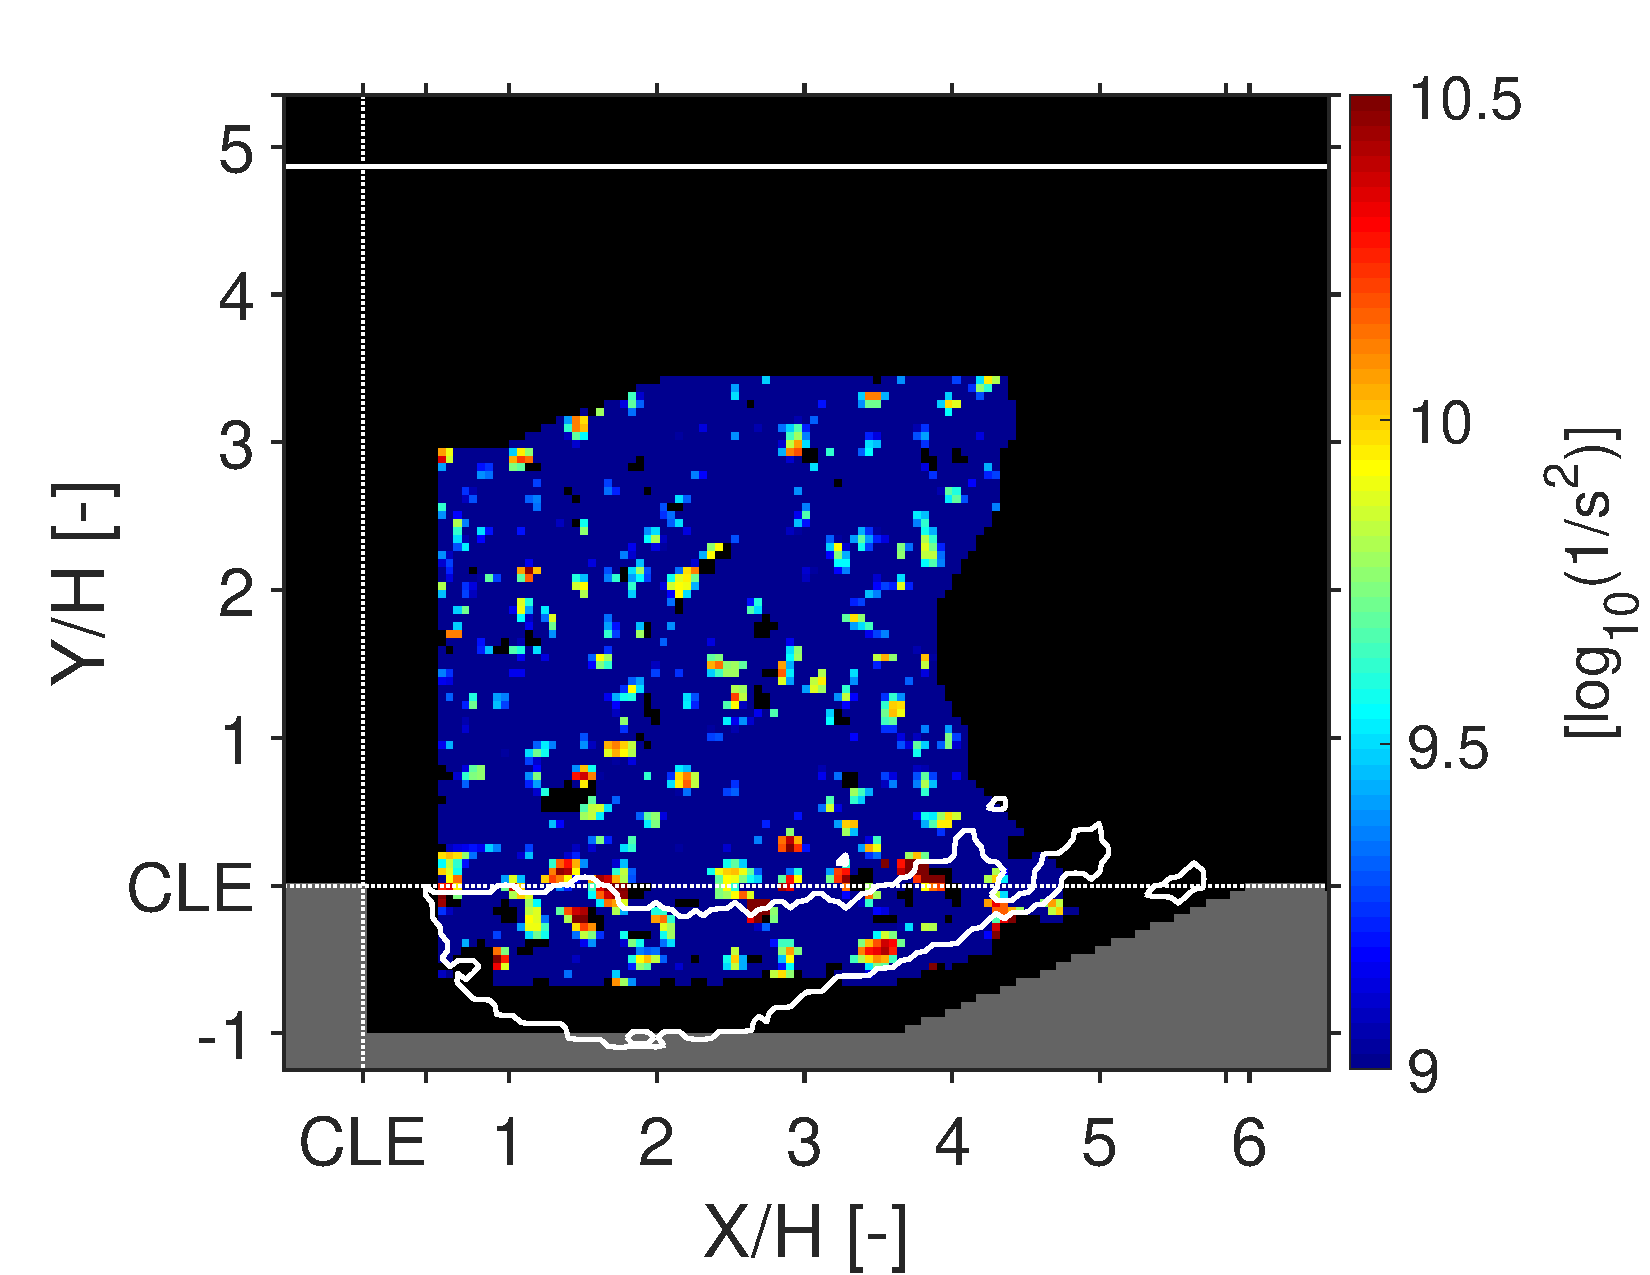
\includegraphics[width=3.25in]{figures/B1/B1_swirling_strength/B1_Frame399.pdf}} \\
\subcaptionbox{State 3\label{fig:B1_R3_ST}}{
        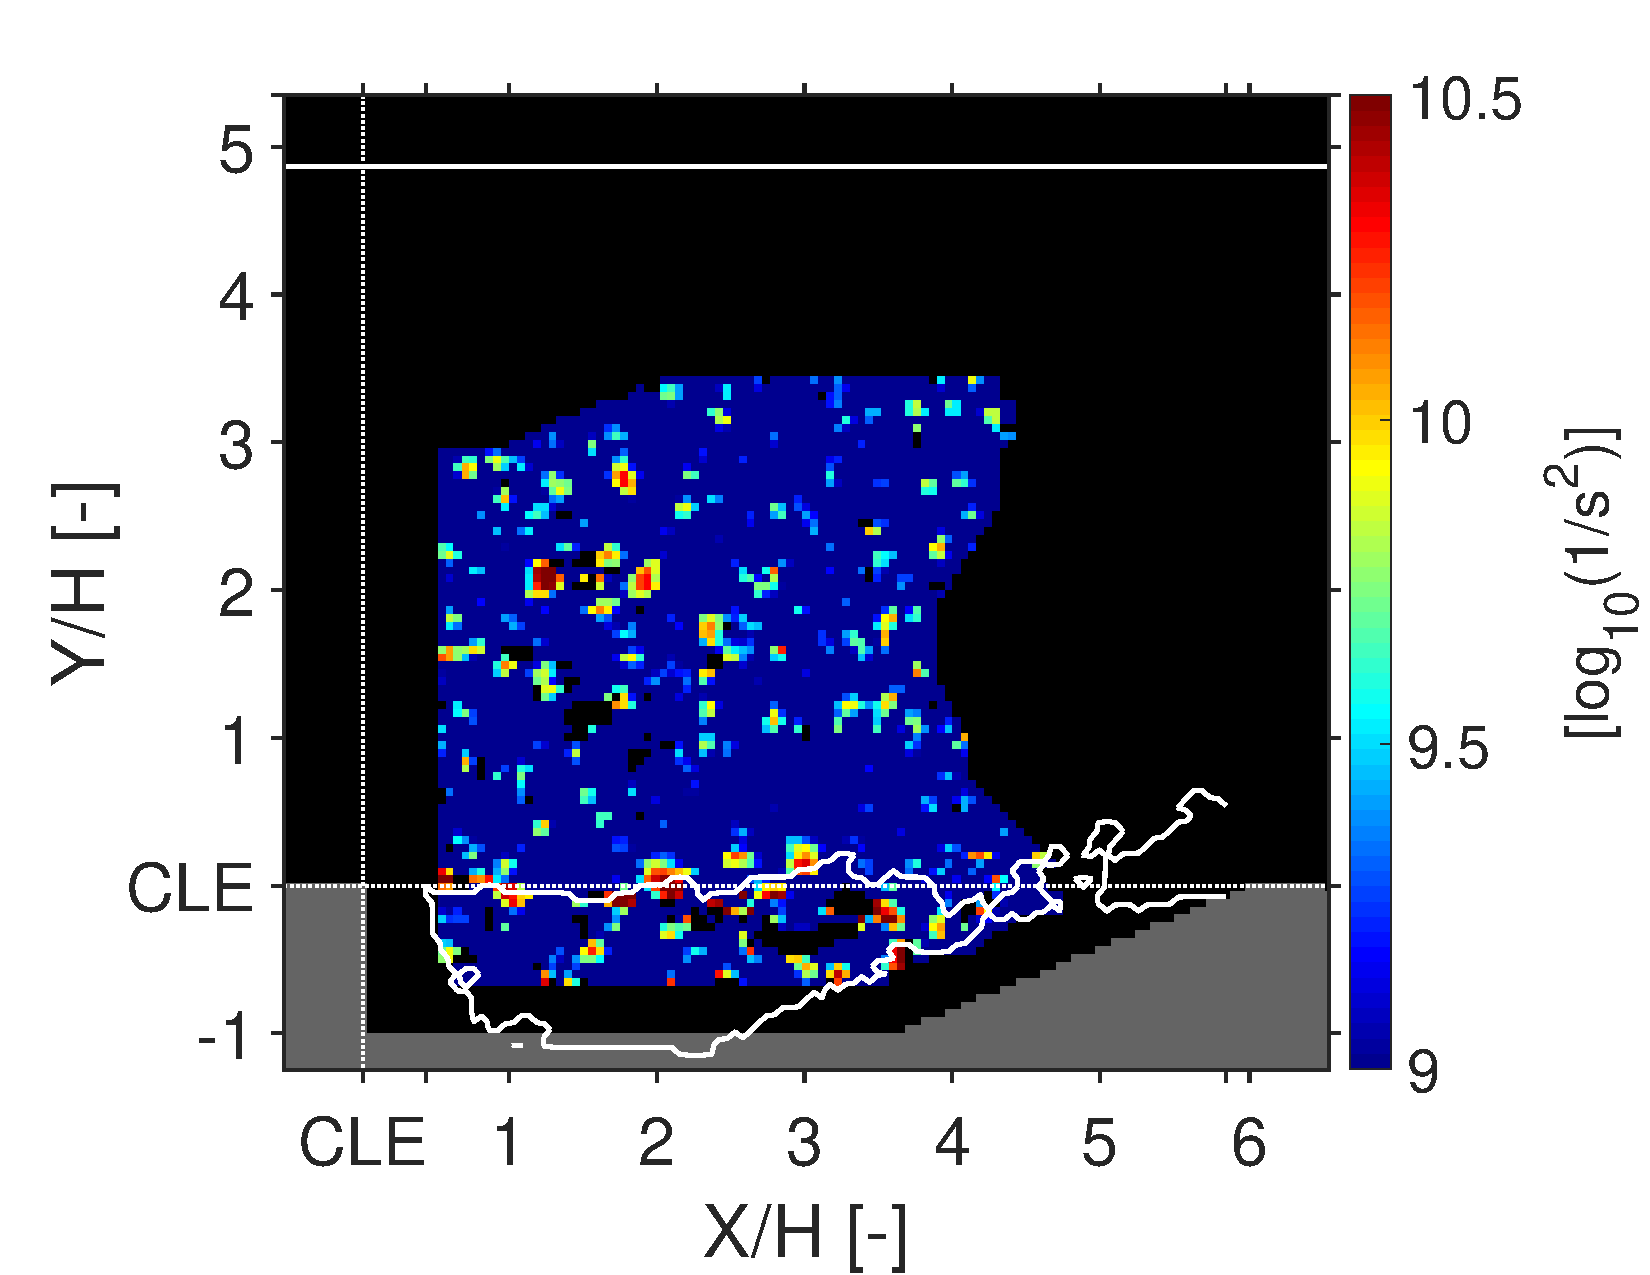
\includegraphics[width=3.25in]{figures/B1/B1_swirling_strength/B1_Frame17.pdf}}
\caption{Select instantaneous swirling strength.}
\label{fig:ch3_inst_ST}
\end{figure}

\citet{AllisonFredericksonKirikEtAl2017} demonstrated the presence of a combustion oscillation at 340 Hz in a similar dual-mode scramjet flowpath with a cavity flameholder using 50 kHz CH* chemiluminescence. These authors attributed the oscillation to thermoacoustic waves between the shock train and thermal throat. They also located the greatest variations in heat release in the region of the flame brush above the ramp. The measured 340 Hz frequency is close to the 357 Hz oscillation frequency detected in the companion LES \citep{ramesh2015large}. Evidence of a similar oscillation is observed in LES applied to the present flowpath \citep{Nielsen2019}, where periodic flame structures ejected from the cavity can also be observed. It is therefore expected that the present flow is subject to thermoacoustic oscillation between the shock train and combustion region (see \citet{MatsuoMiyazatoKim1999} and \citet{WangWangSun2014}). 

%The hypothetical cycle consists of three typical flow states: a cavity-enclosed flame (state 1), a stretched flame extending past the cavity ramp and interface (state 2), which subsequently leads to the ejection of products (state 3). This order is illustrated in Fig. \ref{fig:cycle_diagram} corresponding to the sequence of Figs. \ref{fig:B1_Frame1} to \ref{fig:B1_Frame5}. 

In state 1 (Fig. \ref{fig:B1_Frame1}), the cavity gases are contained within the cavity by the high momentum of the duct flow, leading to shear layer impingement on the cavity ramp. The cavity recirculation zone consists of two large clockwise vortices, expected to grow from the merging of smaller eddies formed at the impingement location \citep{TuttleCarterHsu2014, Kirik2017}. Mass exchange between the duct flow and the cavity flow is low as it occurs mostly through the shear layer rather than along the ramp. Generated heat is thus mostly stored in the cavity by the trapped recirculation zone. During this flow state, some heat may escape at the shear layer impingement zone along the ramp (hidden to the PIV-PLIF cameras due to setup constraints). 

State 1 is unsustainable due to the mass and heat accumulation into the cavity. The shear layer is subsequently lifted (Fig. \ref{fig:B1_Frame2}) and detaches from the cavity ramp. An open question is whether this event is triggered by reaching a threshold in the cavity pressure and gas expansion, or by large-scale flow fluctuations from e.g. shock train fluctuations. 
The lifted shear layer provides an escape route for the trapped gases (state 2). During this event, combustion radicals and products are ejected through a narrow streamtube between the ramp and the lifted shear layer.
The ejection leads to a transfer of heat and mass from the cavity to the duct while stretching the reaction front. 
The flamefront is stretched thinnest between the two large recirculation eddies, leading to breaking of the flame front and detachment of a region of combustion products (Fig. \ref{fig:B1_Frame4}). The above events constitute state 3. Transition back to state 1 occurs as the downstream eddy is convected away by the main flow (Fig. \ref{fig:B1_Frame5}). The shear layer attaches itself back to the ramp, trapping combustion products and radicals in the cavity again. The pressure rise at the reattachment point may shift the upstream eddy towards the cavity leading edge, and a new eddy is formed from the merging of eddies created at the impingement area as suggested by \cite{TuttleCarterHsu2014}. Alternatively, a new eddy may be formed near the cavity leading edge. In this case, the upstream eddy from the previous cycle becomes the new downstream eddy. The proposed cycle is diagrammed in Fig. \ref{fig:cycle_diagram}. 

\begin{figure}
\centering
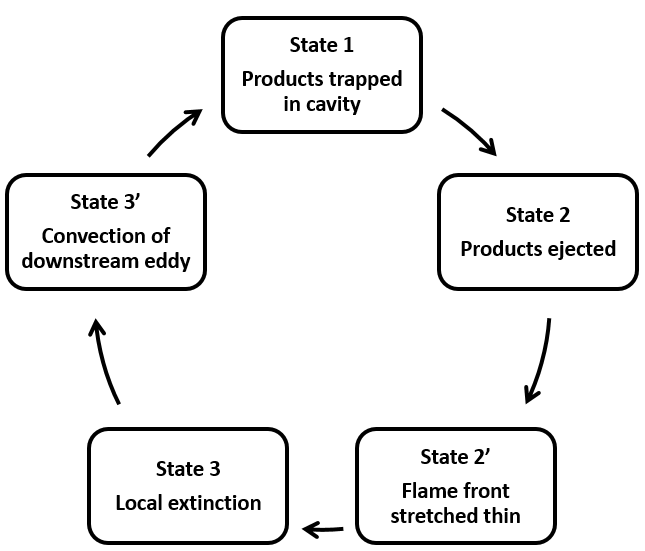
\includegraphics[width=3.25in]{figures/cycle_diagram.png}
\caption{Diagram of the hypothetical combustion cycle.}
\label{fig:cycle_diagram}
\end{figure}

The presence of both positive and negative velocity fluctuations $U'=U-U_{AVG}$ for a same phase, e.g. phase 2 in Fig. \ref{fig:B1_Frame6} versus \ref{fig:B1_Frame2}, suggests a repetition of the cavity combustion cycle within one shock train cycle. Further investigations with high-frequency pressure measurements and LES are warranted to explore the driving factors for the observed cavity combustion oscillation. 

\section*{Conclusions}
The first combined PIV-PLIF measurements in a dual-mode scramjet combustor are presented, giving new insight into an unsteady flame that is stabilized on a cavity in a high speed, premixed flow, and contributing to experimental databases suitable for validation of computational models for such flows.  The flow geometry is explicitly sized to be suitable for DNS modeling. The cavity flow is characterized by an unsteady shear layer and a recirculation zone that exhibits a long period cycle, with scales much larger than the eddy sizes associated with the shear layer above the cavity. This cycle was identified by categorizing PLIF images by common flamefront traits, then sorting them based on the companion velocimetry and physical plausibility. This proposed cycle starts with a trapped vortex that accumulates mass and heat in the cavity. The accumulation is unsustainable and the trapped vortex splits, triggering eventual detachment of the shear layer from the cavity ramp and the ejection of combustion products. As these ejected combustion products move out of the cavity, the flame is broken and products are shed into the duct flow. The shear layer then reattaches and resets the cavity to the trapped vortex state. These observations are consistent with previous work on similar cavity-stabilized flames using non-simultaneous PIV and PLIF. It is speculated that this cavity cycle is phase locked to thermoacoustic oscillations arising from acoustic interaction between the shock train in the inlet isolator and the thermal throat downstream of the cavity.  More experiments with high speed diagnostics are needed to better understand the coupling of the cavity-stabilized combustion dynamics with global instabilities of the engine. Large eddy simulations will also deliver valuable insights into the oscillations across wide temporal and spatial scales. Improving understanding of dual-mode scramjet combustion dynamics in this manner may lead to innovative flameholder geometries and active or passive dampeners for operational scramjet propulsion systems.


\section*{Funding sources}

This research is supported by the Air Force Office of Scientific Research award \#FA9550-15-0440 (technical monitor Dr. Chiping Li) and the National Science Foundation award \#1511520 (program officer Dr. Song-Charng Kong). Clayton Geipel was supported by fellowship awards from the Virginia Space Grant Consortium and the Jefferson Scholars Foundation.

\section*{Acknowledgements}

The authors appreciate the assistance of Dr. Robert Rockwell in operating the UVaSCF for the experiments. They also wish to thank Dr. Vladimir Mitkin for his advice concerning the hypothetical combustion cycle.

\bibliography{references}

\end{document}
